\documentclass[11pt]{article}

% if you need to pass options to natbib, use, e.g.:
%\PassOptionsToPackage{numbers}{natbib}
\usepackage{bm,amsmath,amsthm,amssymb,multicol,algorithmic,algorithm,enumitem,subfigure}
\usepackage{xargs}
\usepackage{stmaryrd}
\usepackage{natbib}
\usepackage{comment}
\usepackage{microtype}
\usepackage{booktabs} % for professional tables


\usepackage{booktabs}       % professional-quality tables
\usepackage{amsfonts}       % blackboard math symbols
\usepackage{multirow}
\usepackage{makecell}
\usepackage{pifont}
\usepackage{mathtools}
\usepackage{balance}

\usepackage{xcolor}
\usepackage{tikz}
\usetikzlibrary{tikzmark,calc}
% ready for submission
\usepackage{neurips_2021}


\DeclarePairedDelimiter{\ceil}{\lceil}{\rceil}
\DeclarePairedDelimiter{\floor}{\lfloor}{\rfloor}
\newcommand{\pl}{Polyak-\L{}ojasiewicz}
\newcommand{\todoM}[1]{\textcolor{blue}{ToDo (Farzin): #1}}
\newcommand{\todo}[1]{\textcolor{red}{ToDo:~#1}}
\newcommand{\alert}[1]{\textcolor{red}{#1}}
\newcommand{\Var}{\mathrm{Var}}
\newcommand{\E}{\mathrm{E}}
\newtheorem{theorem}{Theorem}
\newtheorem{lemma}{Lemma}
\newtheorem{remark}{Remark}
\newtheorem{assumption}{Assumption}
\newtheorem{proposition}{Proposition}
\newtheorem{property}{Property}
\newtheorem{corollary}{Corollary}
\newtheorem{definition}{Definition}
\newtheorem{claim}[theorem]{\bf Claim}
\newtheorem{fact}[theorem]{Fact}
\newtheorem{example}[theorem]{Example}

\newcommand*{\Scale}[2][4]{\scalebox{#1}{$#2$}}%
\newcommand*{\Resize}[2]{\resizebox{#1}{!}{$#2$}}%
\allowdisplaybreaks
\newcommand\DrawBoxhom[3][]{%
  \begin{tikzpicture}[remember picture,overlay]
    \draw[overlay,fill=gray!30,#1] 
    ([xshift=-0.5em,yshift=-0.1ex]{pic cs:#2}) 
    rectangle 
    ([xshift=35pt,yshift=3.1ex]pic cs:#3);
  \end{tikzpicture}%
}


\newcommand\DrawBoxxhom[3][]{%
  \begin{tikzpicture}[remember picture,overlay]
    \draw[overlay,fill=gray!30,#1] 
    ([xshift=-5.9em,yshift=-1.1ex]{pic cs:#2}) 
    rectangle 
    ([xshift=80pt,yshift=-1.5ex]pic cs:#3);
  \end{tikzpicture}%
}


\newcommand\DrawBox[3][]{%
  \begin{tikzpicture}[remember picture,overlay]
    \draw[overlay,fill=gray!30,#1] 
    ([xshift=10em,yshift=-0.4ex]{pic cs:#2}) 
    rectangle 
    ([xshift=-4pt,yshift=1.1ex]pic cs:#3);
  \end{tikzpicture}%
}


\newcommand\DrawBoxx[3][]{%
  \begin{tikzpicture}[remember picture,overlay]
    \draw[overlay,fill=gray!30,#1] 
    ([xshift=-8.0em,yshift=-1.0ex]{pic cs:#2}) 
    rectangle 
    ([xshift=50pt,yshift=-1.2ex]pic cs:#3);
  \end{tikzpicture}%
}


\begin{document}
\title{\texttt{FedSKETCH}: Communication-Efficient Federated Learning via Sketching}



\author{
 Farzin Haddadpour \\
  \texttt{} 
   \And
  Belhal Karimi \\
  Cognitive And Computing Lab\\
  Baidu Research\\
  Beijing, China \\
  \texttt{v_karimibelhal@baidu.com} 
   \And
    Xiaoyun Li \\
  Cognitive And Computing Lab\\
  Baidu Research\\
  Beijing, China \\
  \texttt{v_karimibelhal@baidu.com} 
      \And
  Ping Li \\
  Cognitive And Computing Lab\\
  Baidu Research\\
  Beijing, China \\
  \texttt{liping@baidu.com} \\
}


\date{\today}

\maketitle


\begin{abstract}
Communication complexity and data privacy are the two key challenges in Federated Learning (FL) where the goal is to perform a distributed learning through a large volume of devices. In this work, we introduce two new algorithms, namely \texttt{FedSKETCH} and \texttt{FedSKETCHGATE}, to address jointly both challenges and which are, respectively, intended to be used for homogeneous and heterogeneous data distribution settings. Our algorithms are based on a key and novel sketching technique, called \texttt{HEAPRIX} that is unbiased, compresses the accumulation of local gradients using count sketch, and exhibits communication-efficiency properties leveraging low-dimensional sketches. We provide sharp convergence guarantees of our algorithms and validate our theoretical findings with various sets of experiments. 
\end{abstract}
%\todo{Clarifying cross-device and cross-silo settings}
\vspace{-0.2in}
\section{Introduction}
\vspace{-0.05in}
Federated Learning (FL) is a recently emerging framework for distributed large scale machine learning problems.
In FL, data is distributed across devices~\citep{mcmahan2016communication,konevcny2016federated} and due to privacy concerns, users are only allowed to communicate with the parameter server.
Formally, the optimization problem across $p$ distributed devices is defined as follows:
\begin{align}\label{eq:main}
   \min_{\boldsymbol{x}\in \mathbb{R}^{d},\: \sum_{j=1}^pq_j=1} f(\boldsymbol{x})\triangleq \sum_{j=1}^{p}q_jF_j(\boldsymbol{x}) \, , 
\end{align}
where $F_j(\boldsymbol{x})=\mathbb{E}_{\xi\in\mathcal{D}_j}\left[L_j\left(\boldsymbol{x},\xi\right)\right]$ is the local cost function at device $j$, $q_j\triangleq\frac{n_j}{n}$, $n_j$ is the number of data shards at device $j$ and $n=\sum_{j=1}^pn_j$ is the total number of data samples,
$\xi$ is a random variable distributed according to probability distribution $\mathcal{D}_j$, and $L_j$ is a loss function that measures the performance of model $\boldsymbol{x}$ at device $j$. 
We note that, while for the homogeneous setting we assume $\{\mathcal{D}_j\}_{j=1}^p$ have the same distribution across devices and $L_i=L_j \ , \ 1 \leq (i,j) \leq p$, in the heterogeneous setting, these distributions and loss functions $L_j$ can vary from a device to another. 
% The parameter server orchestrates optimization among devices by aggregating gradient-related information of devices and broadcasts the average of received vectors. 
% Besides, moving data across the devices during the learning a global model can be costly and could violate the privacy of user devices~\citep{carlini2019secret,mcmahan2017learning}. 


There are several challenges that need to be addressed in FL in order to efficiently learn a global model that performs well in average for all devices:

-- \emph{Communication-efficiency}: There are often many devices communicating with the server, thus incurring immense communication overhead. 
One approach to reduce communication round is using \emph{local SGD with periodic averaging}~\citep{zhou2018convergence,stich2019local,yu2019parallel,wang2018cooperative} which periodically averages models after few local updates, contrary to baseline SGD~\citep{bottou-bousquet-2008} where model averaging is performed at each iteration.
Local SGD has been proposed in~\citet{mcmahan2016communication,konevcny2016federated} under the FL setting and its convergence analysis is studied in~\citet{stich2019local,wang2018cooperative,zhou2018convergence,yu2019parallel}, later on improved in the follow up references~\citep{basu2019qsparse,haddadpour2019convergence,bayoumi2020tighter,stich2019error} for homogeneous setting. 
It is further extended to heterogeneous setting~\citep{yu2019linear,li2019convergence,sahu2018convergence,liang2019variance,haddadpour2019convergence,karimireddy2019scaffold}. Second approach to deal with communication cost aims at reducing the size of communicated message per communication round, such as local gradient quantization~\citep{alistarh2017qsgd,bernstein2018signsgd,tang2018communication,wen2017terngrad,wu2018error} or sparsification~\citep{alistarh2018convergence,lin2017deep,stich2018sparsified,stich2019error}. 
%Additionally, similar Local SGD with adaptive gradient methods can be found in~\citet{reddi2020adaptive,chen2020toward}.


--\emph{Data heterogeneity}: 
Since locally generated data in each device may come from different distribution, local computations involved in FL setting can lead to poor convergence error in practice~\citep{li2019federated,liang2019variance}. 
To mitigate the negative impact of data heterogeneity,~\citep{haddadpour2020federated,horvath2019stochastic,liang2019variance,karimireddy2019scaffold} suggest applying variance reduction or gradient tracking techniques along local computations.

 --\emph{Privacy}~\citep{geyer2017differentially,hardy2017private}: Privacy has been widely addressed by injecting an additional layer of randomness to respect differential-privacy property~\citep{mcmahan2017learning} or using cryptography-based approaches under secure multi-party computation~\citep{bonawitz2017practical}. 
  Further study of challenges can be found in recent surveys~\cite{li2020federated} and~\cite{kairouz2019advances}.
%One approach to deal with communication cost is the idea of \emph{local SGD with periodic averaging}~\citep{zhou2018convergence,stich2019local,yu2019parallel,wang2018cooperative} which asserts that instead of taking the average within each iteration, like baseline SGD~\citep{bottou-bousquet-2008}, one may take the average periodically and performs local update, see local SGD~\citep{lin2019don}. 
%It is shown that local SGD with periodic averaging benefits from the same convergence rate as baseline SGD, while requiring less communication rounds. 
%The second approach to deal with communication cost aims at reducing the size of communicated message per communication round. 
%Available methods reduce the size of the message by communicating compressed local gradients or models to parameter server via quantization~\citep{alistarh2017qsgd,bernstein2018signsgd,tang2018communication,wen2017terngrad,wu2018error}, sparsification~\citep{alistarh2018convergence,lin2017deep,stich2018sparsified,stich2019error}.%, or combination of both~\citep{basu2019qsparse}.
%A large amount of research efforts, such as~\citep{liang2019variance,karimireddy2019scaffold,horvath2019stochastic,haddadpour2020federated} aim at mitigating the effect of data heterogeneity by exploiting variance reduction or gradient tracking techniques in distributed optimization settings where data distribution is non-iid.
%Solving the privacy issue has been widely performed by injecting an additional layer of random noise in order to respect differential-privacy property of the method~\citep{mcmahan2017learning} or using cryptography-based approaches under secure multi-party computation~\citep{bonawitz2017practical} framework.
%Almost all of the previous studies consider addressing the aforementioned challenges separately. 


To tackle all major aforementioned challenges in FL jointly, sketching based algorithms~\citep{DBLP:journals/tcs/CharikarCF04,cormode2005improved,kleinberg2003bursty,Proc:Li_Church_Hastie_NIPS08} 
are promising approaches. 
%Sketches are built from independent hash tables (functions), compressing a high dimensional vector into a lower dimensional one and the corresponding estimation error of sketching are well studied. 
For instance, to reduce communication cost,~\citep{ivkin2019communication} develop a distributed SGD algorithm using sketching along providing its convergence analysis in the homogeneous setting, and establish a communication complexity of order $\mathcal{O}(\log(d))$ per round, where $d$ is the dimension of the vector of parameters compared to $\mathcal{O}(d)$ complexity per round of baseline mini-batch SGD. Yet, the proposed sketching scheme in~\citet{ivkin2019communication}, built from a communication-efficiency perspective, is based on a deterministic procedure which requires access to the exact information of the gradients, thus not meeting the crucial privacy-preserving criteria.
This systemic flaw is partially addressed in~\citet{rothchild2020fetchsgd}. 


Focusing on privacy,~\citep{li2019privacy} derive a single framework in order to tackle these issues jointly and introduces \texttt{DiffSketch} algorithm, based on the Count Sketch operator, yet does not provide its convergence analysis.
Additionally, the estimation error of \texttt{DiffSketch} is higher than the sketching scheme in~\citet{ivkin2019communication} which may end up in poor convergence. 
%~\citep{rothchild2020fetchsgd} considers using sketching technique in heterogeneous setting from a communication-efficiency perspective.
%They introduce \texttt{Sketched-SGD} and establish a communication complexity of order $\mathcal{O}(\log(d))$ (per round) where $d$ is the dimension of the vector of parameters, i.e., the dimension of the gradient.
%Compression methods such as quantized gradients are developed in~\citet{alistarh2017qsgd,lin2017deep,stich2018sparsified,horvath2019stochastic,horvath2020better}. 
 
 In this paper, we propose new sketching algorithms to address the aforementioned challenges simultaneously.
 Our main contributions are summarized as:
\begin{itemize}
    \item We provide a new algorithm -- \texttt{HEAPRIX} -- and theoretically show that it reduces the cost of communication between devices and server, which is based on unbiased sketching without requiring the broadcast of exact values of gradients to the server. 
    Based on \texttt{HEAPRIX}, we develop general algorithms for communication-efficient and sketch-based FL, namely \texttt{FedSKETCH} and \texttt{FedSKETCHGATE} for both homogeneous and heterogeneous data distribution settings respectively.
    \item We establish non-asymptotic convergence bounds for convex, \pl\:(PL) and non-convex functions in Theorems~\ref{thm:homog_case} and~\ref{thm:hetreg_case} in both homogeneous and heterogeneous cases, and highlight an improvement in the number of iteration to reach a stationary point.
We also provide a convergence analysis for the \texttt{PRIVIX} algorithm proposed in~\citet{li2019privacy}.
    \item We illustrate the benefits of \texttt{FedSKETCH} and \texttt{FedSKETCHGATE} over baseline methods through a set of experiments. 
    The latter shows the advantages of the \texttt{HEAPRIX} compression method achieving comparable test accuracy as Federated SGD (\texttt{FedSGD}) while compressing the information exchanged between devices and server.
\end{itemize}


%\vspace{0.05in}
\noindent\textbf{Notation:} 
We denote the number of communication rounds and bits per round and per device by $R$ and $B$ respectively. 
The count sketch of any vector $\boldsymbol{x}$ is designated by $\mathbf{S}(\boldsymbol{x})$. $[p]$ denotes the set $\{1,\dots,p\}$.

\vspace{-0.05in}
\section{Compression using Count Sketch}\label{sec:compression}
\vspace{-0.05in}

In this paper, we exploit the commonly used \texttt{Count Sketch} ~\citep{DBLP:journals/tcs/CharikarCF04} which uses two sets of functions that encode any input vector $\boldsymbol{x}$ \textbf{into a hash table} $\boldsymbol{S}_{m\times t}(\boldsymbol{x})$. 
Pairwise independent hash functions $\{h_{j,1\leq j\leq t }:[d]\rightarrow m\}$ are used along with another set of pairwise independent sign hash functions $\{\text{sign}_{j,1\leq j\leq t}: [d]\rightarrow \{+1,-1\}\}$ to map entries of $\boldsymbol{x}$ (${x}_i, \:1\leq i\leq d$) into $t$ different columns of $\mathbf{S}_{m\times t}$, wherein to lower the dimension of the input vector we usually have $d\gg mt$.  
The final update reads $\mathbf{S}[j][h_j(i)]=\mathbf{S}[j-1][h_{j-1}(i)]+\text{sign}_j(i).{x}_i$ for any $1 \leq j \leq t$ .
There are various types of sketching algorithms which are developed based on count sketching that we develop in the following subsections. 
See the Appendix for the detailed Count Sketch algorithm. 




\vspace{-0.05in}
\subsection{Sketching based Unbiased Compressor}
\vspace{-0.05in}



We define an unbiased compressor as follows:
\begin{definition}[Unbiased compressor]\label{def:unbiased}
A randomized function, $\text{C}:\mathbb{R}^{d}\rightarrow\mathbb{R}^{d}$ is called an unbiased compression operator with $\Delta\geq 1$, if we have 
\begin{align}\notag
\mathbb{E}\left[\text{C}(\boldsymbol{x})\right]&=\boldsymbol{x}\nonumber \quad \textrm{and} \quad    \mathbb{E}\left[\left\|\text{C}(\boldsymbol{x})\right\|^2_2\right] \leq \Delta\left\|\boldsymbol{x}\right\|^2_2\notag \, .
\end{align}
We denote this class of compressors by $\mathbb{U}(\Delta)$.
\end{definition}
This definition leads to the following property 
\begin{align}\notag
    \mathbb{E}\left[\left\|\text{C}(\boldsymbol{x})-\boldsymbol{x}\right\|^2_2\right]&\leq \left(\Delta-1\right)\left\|\boldsymbol{x}\right\|^2_2\, .
\end{align}
Note that if we let $\Delta=1$ then our algorithm reduces to the case of no compression. 
This property allows us to control the noise of the compression.
%%%%%%%%%%%%%%%%%%%%%%%%%%%%%%%%%%%%%%
%%%%%%%%%%%%%%%%%%%%%%%%%%%%%%%%%%%%%%%

%\textit{An Example of Unbiased Compressor via Sketching:}
An instance of such unbiased compressor is \texttt{PRIVIX} which obtains an estimate of input $\boldsymbol{x}$ from a count sketch noted $\boldsymbol{S}(\boldsymbol{x})$. 
In this algorithm, to query the quantity $x_i$, the $i-th$ element of the vector $\boldsymbol{x}$, we compute the median of $t$ approximated values specified by the indices of $h_j(i)$ for $1\leq j\leq t$, see~\citep{li2019privacy} or Algorithm~\ref{Alg:privix} in the Appendix (for more details).
%\begin{algorithm}[t]
%\caption{\texttt{PRIVIX}~\citep{li2019privacy}: Unbiased compressor based on sketching. }\label{Alg:privix}
%\begin{algorithmic}[1]
%\STATE\textbf{Inputs:} $\boldsymbol{x}\in\mathbb{R}^{d}, t, m, \mathbf{S}_{m\times t}, h_j (1\leq i\leq t), sign_j (1\leq i\leq t)$
%\STATE\textbf{Query} $\tilde{\boldsymbol{x}}\in\mathbb{R}^d$ \textbf{from $\mathbf{S(\boldsymbol{x})}$:}
%\STATE\textbf{for} $i=1,\ldots,d$ \textbf{do}
%\STATE\quad\quad ${\tilde{\boldsymbol{x}}}[i]=\text{Median}\{\text{sign}_j(i).\mathbf{S}[j][h_j(i)]:1\leq j\leq t\}$ 
%\STATE\textbf{end for}
%\STATE\textbf{Output:} ${\tilde{\boldsymbol{x}}}$
%\vspace{- 0.1cm}
%\end{algorithmic}
%\end{algorithm}
%%%%%%%%%%%%%%%%%%%%%%%%%%%%%%%%%%%%%%%%%%
% Next, we review a few properties of \texttt{PRIVIX}: 
% \vspace{0.1in}\noindent\textbf{Estimation errors:}
For the purpose of our proof, we state the following crucial properties of the count sketch:
%\begin{property}[\citep{li2019privacy}]
%For any $\mathbf{x}\in \mathbb{R}^{d}$, $\texttt{PRIVIX}$ is unbiased: $\mathbb{E}_{\mathbf{S}}\left[\texttt{PRIVIX}\left[\mathbf{S}\left(\mathbf{x}\right)\right]\right]=\mathbf{x}$ and has \emph{bounded variance}: $\mathbb{E}_{\mathbf{S}}[\|\texttt{PRIVIX}[\mathbf{S}(\mathbf{x})]-\mathbf{x}\|_2^2]\leq \mu^2 d\|\mathbf{x}\|_2^2, \: \textrm{w.p.} \: 1-\delta$, if $m=\mathcal{O}\left(\frac{e}{\mu^2}\right)$, $t=\mathcal{O}\left(\ln \left(\frac{d}{\delta}\right)\right)$.
%\end{property}
\begin{property}[\citet{li2019privacy}]
For any $\boldsymbol{x}\in \mathbb{R}^{d}$, we have:

\textit{Unbiased estimation}: As in~\citet{li2019privacy}, we have:
    \begin{align}\notag
        \mathbb{E}_{\mathbf{S}}\left[\texttt{PRIVIX}\left[\mathbf{S}\left(\boldsymbol{x}\right)\right]\right]=\boldsymbol{x}\, .
    \end{align}
\textit{Bounded variance:} For the given $m<d$, $t=\mathcal{O}\left(\ln \left(\frac{d}{\delta}\right)\right)$ with probability $1-\delta$ we have:
    \begin{align}\notag
        \mathbb{E}_{\mathbf{S}}\left[\left\|\texttt{PRIVIX}\left[\mathbf{S}\left(\boldsymbol{x}\right)\right]-\boldsymbol{x}\right\|_2^2\right] \leq c\frac{d}{m}\left\|\boldsymbol{x}\right\|_2^2\ , 
    \end{align}
 where $c$ ($e\leq c<m$) is a positive constant independent of the dimension of the input, $d$.
\end{property}
Thus, with probability $1-\delta$ we obtain that $\texttt{PRIVIX}\in \mathbb{U}(1+c\frac{d}{m})$.
Note $\Delta=1+c\frac{d}{m}$ implies that if $m\rightarrow d$, then $\Delta\rightarrow 1+c$, indicating a noisy reconstruction. 
Exploiting this noisy reconstruction, \citet{li2019privacy} show that if the data is normally distributed, \texttt{PRIVIX} is differentially private~\citep{DBLP:conf/icalp/Dwork06}, up to additional assumptions and algorithmic design.  


\vspace{-0.05in}
\subsection{Sketching based Biased Compressor}
\vspace{-0.05in}

A biased compressor is defined as follows:
\begin{definition}[Biased compressor]
A (randomized) function,  ${\text{C}}:\mathbb{R}^{d}\rightarrow\mathbb{R}^{d}$ belongs to $\mathbb{C}(\Delta,\alpha)$, a class of compression operators with $\alpha>0$ and $\Delta\geq 1$, if
\begin{align}\notag
    \mathbb{E}\left[\left\|\alpha\boldsymbol{x}-{\text{C}}(\boldsymbol{x})\right\|^2_2\right]\leq \left(1-\frac{1}{\Delta}\right)\left\|\boldsymbol{x}\right\|^2_2\, ,
\end{align}
%We denote this class of biased operators by $\mathbb{C}(\Delta,\alpha)$. 
\end{definition}
The reference~\citep{horvath2020better} proves that $\mathbb{U}(\Delta)\subset\mathbb{C}(\Delta, \alpha)$.
%The following Lemma links these two definitions:
%\begin{lemma}[\citep{horvath2020better}]
%We have $\mathbb{U}(\Delta)\subset\mathbb{C}(\Delta, \alpha)$.
%\end{lemma}
An example of biased compression via sketching and using top$_m$ operation is given below:
%%%%%%%%%%%%%%%%%%%%%%%%%%%%%%%%%%
\begin{algorithm}[H]
\caption{\texttt{HEAVYMIX}  }\label{alg:heavymix}
\begin{algorithmic}[1]
\STATE \textbf{Inputs:} $\mathbf{S}({\mathbf{g}})$; parameter $m$
\STATE {Query the vector $\tilde{\mathbf{g}}\in\mathbb{R}^{d}$ from $\mathbf{S}\left(\mathbf{g}\right)$:}
\STATE Query $\hat{\ell}_2^2=\left(1\pm 0.5\right)\left\|\mathbf{g}\right\|^2$ from sketch $\mathbf{S}(\mathbf{g})$
\STATE $\forall j$ query $\hat{\mathbf{g}}_j^2=\hat{\mathbf{g}}_j^2\pm \frac{1}{2m}\left\|\mathbf{g}\right\|^2$ from sketch $\mathbf{S}(\mathbf{g})$
\STATE $H=\{j|\hat{\mathbf{g}}_j\geq \frac{\hat{\ell}_2^2}{m}\}$ and $NH=\{j|\hat{\mathbf{g}}_j<\frac{\hat{\ell}_2^2}{m}\}$
\STATE Top$_m=H\cup \text{rand}_\ell(NH)$, where $\ell=m-\left|H\right|$
\STATE Get exact values of Top$_m$ 
\STATE \textbf{Output:} $\tilde{\mathbf{g}}:\forall j\in\text{Top}_m:\tilde{\mathbf{g}}_{i}=\mathbf{g}_{i}$ else $ \mathbf{g}_{i}=0$
%\vspace{- 0.1cm}
\end{algorithmic}
\end{algorithm}
%%%%%%%%%%%%%%%%%%%%%%%%%%%%%%%%%%%%%%%%%%
Following~\citet{ivkin2019communication}, \texttt{HEAVYMIX} with sketch size $\Theta\left(m\log\left(\frac{d}{\delta}\right)\right)$ is a biased compressor with $\alpha=1$ and  $\Delta=d/m$ with probability $\geq1-\delta$. In other words, with probability $1-\delta$, $\texttt{HEAVYMIX}\in C(\frac{d}{m},1)$. 
%\begin{lemma}[\citep{ivkin2019communication}]
%\texttt{HEAVYMIX}, with sketch size $\Theta\left(m\log\left(\frac{d}{\delta}\right)\right)$ is a biased compressor with $\alpha=1$ and  $\Delta=d/m$ with probability $\geq1-\delta$. In other words, with probability $1-\delta$, $\texttt{HEAVYMIX}\in C(\frac{d}{m},1)$. 
%\end{lemma}
We note that Algorithm~\ref{alg:heavymix} is a variation of the sketching algorithm developed in~\citet{ivkin2019communication} with distinction that \texttt{HEAVYMIX} does not require a second round of communication to obtain the exact values of top$_m$. 
Additionally, while a sketching algorithm implementing \texttt{HEAVYMIX} has smaller estimation error compared to \texttt{PRIVIX}, it requires having access to the exact values of top$_m$, therefore not benefiting from privacy properties contrary to \texttt{PRIVIX}. 
In the following we introduce our sketching scheme -- \texttt{HEAPRIX} -- as a combination of those two methods. 

\vspace{-0.05in}
\subsection{Sketching based Induced Compressor}
\vspace{-0.05in}

Due to Theorem~$3$ in~\citet{horvath2020better}, which illustrates that we can convert the biased compressor into an unbiased one such that, for $C_1\in \mathbb{C}(\Delta_1)$ with $\alpha=1$, if you choose $C_2\in \mathbb{U}(\Delta_2)$, then induced compressor $C: x \mapsto C_1(\mathbf{x})+C_2\left(\mathbf{x}-C_1\left(\mathbf{x}\right)\right)$ belongs to $\mathbb{U}(\Delta)$ with $\Delta=\Delta_2+\frac{1-\Delta_2}{\Delta_1}$. Based on this notion, Algorithm~\ref{alg:heaprix} proposes an induced sketching algorithm by utilizing \texttt{HEAVYMIX} and \texttt{PRIVIX} for $C_1$ and $C_2$ respectively where the reconstruction of input $\mathbf{x}$ is performed using hash table $\mathbf{S}$ and $\mathbf{x}$, similar to \texttt{PRIVIX} and \texttt{HEAVYMIX}.
%%%%%%%%%%%%%%%%%%%%%%%%%%%%%%%%%%
\begin{algorithm}[H]
\caption{\texttt{HEAPRIX} }\label{alg:heaprix}
\begin{algorithmic}[1]
\STATE \textbf{Inputs:} $\boldsymbol{x}\in\mathbb{R}^{d}, t, m, \mathbf{S}_{m\times t}, h_j (1\leq i\leq t), \text{sign}_j (1\leq i\leq t)$, parameter $m$
\STATE {Approximate $\mathbf{S}(\boldsymbol{x})$ using \texttt{HEAVYMIX} }
\STATE {Approximate} $\mathbf{S}\left(\boldsymbol{x} - \texttt{HEAVYMIX}[\mathbf{S}(\boldsymbol{x})]\right)$ using \texttt{PRIVIX} 
\STATE \textbf{Output:}
\vspace{- 0.1cm}
\[ \Resize{7.4cm}{\texttt{HEAVYMIX}\left[\mathbf{S}\left(\boldsymbol{x}\right)\right]+\texttt{PRIVIX}\left[\mathbf{S}\left(\boldsymbol{x}-\texttt{HEAVYMIX}\left[\mathbf{S}\left(\boldsymbol{x}\right)\right]\right)\right]}\ .\]
%\vspace{- 0.1cm}
\end{algorithmic}
\end{algorithm}
%%%%%%%%%%%%%%%%%%%%%%%%%%%%%%%%%%%%%%%%%%
Note that if $m\rightarrow d$, then $C(\boldsymbol{x})\rightarrow \boldsymbol{x}$, which implies that the convergence rate of the algorithm can be improved by decreasing the size of compression $m$. 
\begin{corollary}\label{cor:small}
Based on~Theorem 3 of~\citep{horvath2020better}, \texttt{HEAPRIX} in Algorithm~\ref{alg:heaprix} satisfies $C(\boldsymbol{x})\in \mathbb{U}(c \frac{d}{m})$. 
\end{corollary}
\textit{Benefits of \texttt{HEAPRIX}:} Corollary~\ref{cor:small} states that, unlike \texttt{PRIVIX}, \texttt{HEAPRIX} compression noise can be made as small as possible using larger hash size. 
Contrary to \texttt{HEAVYMIX}, \texttt{HEAPRIX} does not require having access to exact $\text{top}_m$ values of the input, thus helps preserving privacy. 
In other words, \texttt{HEAPRIX} leverages the best of both worlds: the \emph{unbiasedness} of \texttt{PRIVIX} while using \emph{heavy hitters} as in \texttt{HEAVYMIX}.

%In the following we define two general frameworks for different sketching algorithms for homogeneous and heterogeneous data distributions.
\vspace{-0.05in}
\section{\texttt{FedSKETCH} and \texttt{FedSKETCHGATE}}\label{sec:algos}
\vspace{-0.05in}
We define two general frameworks for different sketching algorithms for homogeneous and heterogeneous settings.
%In this section we introduce our two new algorithms for both homogeneous and heterogeneous settings.
\vspace{-0.05in}
\subsection{Homogeneous Setting}
\vspace{-0.05in}

%The proposed algorithms for FL leverage sketching techniques to reduce communication costs.

In \texttt{FedSKETCH}, the number of local updates, between two consecutive communication rounds, at device $j$ is denoted by $\tau$.
 Unlike~\citet{haddadpour2020federated}, server node does not store any global model, rather, device $j$ has two models: $\boldsymbol{x}^{(r)}$ and $\boldsymbol{x}^{(\ell,r)}_j$, which are respectively the local and global models. 
%At communication round $r$ and device $j$, the local model $\boldsymbol{x}^{(\ell,r)}_j$ is updated using the rule $$\boldsymbol{x}_j^{(\ell+1,r)}=\boldsymbol{x}_j^{(\ell,r)}-\eta \tilde{\mathbf{g}}_j^{(\ell,r)} \qquad \text{for}\quad\ell=0,\ldots,\tau-1\, , $$
%where $\tilde{\mathbf{g}}_j^{(\ell,r)}\triangleq\nabla{f}_j(\boldsymbol{x}_j^{(\ell,r)},\Xi_j^{(\ell,r)})\triangleq\frac{1}{b}\sum_{\xi\in\Xi_j^{(\ell,r)}}\nabla{L}_j(\boldsymbol{x}_j^{(\ell,r)},\xi)$ is a stochastic gradient of $f_j$ evaluated using the mini-batch $\Xi_j^{(\ell,r)}=\{\xi^{(\ell,r)}_{j,1},\ldots,\xi^{(\ell,r)}_{j,b_j} \}$ of size $b_j$ and $\eta$ is the local learning rate. After $\tau$ local updates, model at device $j$ and communication round $r$ is indicated by $\boldsymbol{x}_j^{(\tau,r)}$. The next step of our algorithm is that device $j$ sends the count sketch $\mathbf{S}_j^{(r)}\triangleq\mathbf{S}_j\left(\boldsymbol{x}_j^{(\tau,r)}-\boldsymbol{x}_j^{(0,r)}\right)$ back to the server. We note that
% \begin{equation}
% \begin{split}
% \mathbf{S}_j^{(r)} & \triangleq\mathbf{S}_j\left(\boldsymbol{x}_j^{(\tau,r)}-\boldsymbol{x}_j^{(0,r)}\right)\\
% & =\mathbf{S}_j\left(\eta\sum_{\ell=0}^{\tau-1}\tilde{\mathbf{g}}_j^{(\ell,r)}\right)=\eta\mathbf{S}_j\left(\sum_{\ell=0}^{\tau-1}\tilde{\mathbf{g}}_j^{(\ell,r)}\right)\, ,
%\end{split}
%  \end{equation}
% which is the aggregation of the consecutive stochastic gradients multiplied with local updates $\eta$.
%
%Upon receiving all $\mathbf{S}_j^{(r)}$ from sampled devices, the server computes \begin{align}\mathbf{S}^{(r)}=\frac{1}{k}\sum_{j\in\mathcal{K}^{(r)}}\mathbf{S}_j^{(r)}\label{eq:average-skestching}
%\end{align} and broadcasts it to all devices. 
%Devices after receiving $\mathbf{S}^{(r)}$ from server update global model $\boldsymbol{x}^{(r)}$ using rule $$\boldsymbol{x}^{(r)}=\boldsymbol{x}^{(r-1)}-\gamma \texttt{PRIVIX}\left[\mathbf{S}^{(r-1)}\right]\, .$$
We develop \texttt{FedSKETCH} in Algorithm~\ref{Alg:PFLHom}. 
\begin{algorithm}[t]
\DrawBoxhom[draw=white,fill=blue!6]{i}{j}
\DrawBoxxhom[draw=white,fill=blue!6]{k}{l}
\caption{\texttt{FedSKETCH}($R$, $\tau, \eta, \gamma$) }\label{Alg:PFLHom}
\begin{algorithmic}[1]
\STATE \textbf{Inputs:} $\boldsymbol{x}^{(0)}$: initial  model shared by all local devices, global and local learning rates $\gamma$ and $\eta$, respectively
%\STATE Server chooses a subset $\mathcal{P}_0$ of $K$ devices at random (device $j$ is chosen with probability $q_j$);
\STATE \textbf{for $r=0, \ldots, R-1$ do}
\STATE \textbf{parallel for device $j\in \mathcal{K}^{(r)}$ do}:
\STATE \hspace{0.02in} \textbf{if PRIVIX variant:} 
{\small $${\mathbf{\Phi}}^{(r)}\triangleq  {\texttt{PRIVIX}}\left[{\mathbf{S}}^{(r-1)}\right]$$}
\tikzmark{i} 
\STATE \hspace{0.02in} \textbf{if HEAPRIX variant:} \label{line:heaprix1}
{\small $${\mathbf{\Phi}}^{(r)}\triangleq \texttt{HEAVYMIX}\left[{\mathbf{S}}^{(r-1)}\right]+\texttt{PRIVIX}\left[{\mathbf{S}}^{(r-1)}- \tilde{\mathbf{S}}^{(r-1)}\right]$$}
\STATE Set $\boldsymbol{x}^{(r)}=\boldsymbol{x}^{(r-1)}-\gamma{\mathbf{\Phi}}^{(r)}$ and $\boldsymbol{x}_j^{(0,r)}=\boldsymbol{x}^{(r)}$ 
\tikzmark{j}  
\STATE \hspace{0.01in} \textbf{for} $\ell=0,\ldots,\tau-1$ \textbf{do}
\STATE \hspace{0.03in} Sample a mini-batch $\xi_j^{(\ell,r)}$ and compute $\tilde{\mathbf{g}}_{j}^{(\ell,r)}$
\STATE Update $\boldsymbol{x}^{(\ell+1,r)}_{j}=\boldsymbol{x}^{(\ell,r)}_j-\eta~ \tilde{\mathbf{g}}_{j}^{(\ell,r)}$ \label{eq:update-rule-alg}
\STATE \hspace{0.05in}\textbf{end for}
\STATE Device $j$ broadcasts $\mathbf{S}^{(r)}_{j}\triangleq\mathbf{S}_{j}\left(\boldsymbol{x}_j^{(0,r)}-~{\boldsymbol{x}}_{j}^{(\tau,r)}\right)$.
\STATE Server \textbf{computes} $ {\mathbf{S}}^{(r)}=\frac{1}{k}\sum_{j\in\mathcal{K}}\mathbf{S}^{(r)}_{j}$ .\label{line:heaprix2}
\STATE Server \textbf{broadcasts} ${\mathbf{S}}^{(r)}$ to devices in randomly drawn devices $\mathcal{K}^{(r)}$.
\vspace{0.1cm}
\tikzmark{k}  
\STATE \hspace{0.04in} \textbf{if HEAPRIX variant:} 
\STATE $\quad$ Second round of communication: $\mathbf{\delta}_j^{(r)} :=  \mathbf{S}_j\left[\texttt{HEAVYMIX}(\mathbf{S}^{(r)})\right]$ and broadcasts $\tilde{\mathbf{S}}^{(r)}\triangleq\frac{1}{k}\sum_{j\in\mathcal{K}}\mathbf{\delta}_j^{(r)}$ to devices in set $\mathcal{K}^{(r)}$
\tikzmark{l}  
\vspace{0.1cm}
\STATE \textbf{end parallel for}
\STATE \textbf{end}
\STATE \textbf{Output:} ${\boldsymbol{x}}^{(R-1)}$
\vspace{- 0.1cm}
\end{algorithmic}
\end{algorithm}
A variant of this algorithm implementing \texttt{HEAPRIX} is also described in Algorithm~\ref{Alg:PFLHom}. 
We note that for this variant, we need to have an additional communication round between server and worker $j$ to aggregate $\mathbf{\delta}_j^{(r)}\triangleq \mathbf{S}_j\left[\texttt{HEAVYMIX}(\mathbf{S}^{(r)})\right]$, see Lines~\ref{line:heaprix1} and~\ref{line:heaprix2}. The main difference between our \texttt{FedSKETCH} and the \texttt{DiffSketch} algorithm in~\citet{li2019privacy} is that we use distinct local and global learning rates. Furthermore, unlike~\citet{li2019privacy}, we do not add local Gaussian noise. 




\noindent\textbf{Algorithmic comparison  with~\citet{haddadpour2020federated}}
An important feature of our algorithm is that due to a lower dimension of the count sketch, the resulting averages ($\mathbf{S}^{(r)}$ and  $\tilde{\mathbf{S}}^{(r)}$) received by the server, are also of lower dimension. 
Therefore, these algorithms exploit a bidirectional compression during the communication from server to device back and forth. 
As a result, due to this bidirectional property of communicating sketching for the case of large quantization error $\omega=\theta(\frac{d}{m})$ as shown in~\citet{haddadpour2020federated}, our algorithms can outperform \texttt{FedCOM} and \texttt{FedCOMGATE} developed in~\citet{haddadpour2020federated} if sufficiently large hash tables are used and the uplink communication cost is high. 
Furthermore, while, in~\citet{haddadpour2020federated}, server stores a global model and aggregates the partial gradients from devices which can enable the server to extract some information regarding the device's data, in contrast, in our algorithms server does not store the global model and only broadcasts the average sketches. 
Thus, sketching-based server-devices communication algorithms such as ours do not reveal the exact values of the inputs, to preserve privacy as a by-product.

\begin{remark}
As pointed out in~\cite{horvath2020better}, while induced compressors transform a biased compressor into unbiased one, as a drawback it doubles communication cost since the devices need to send $C_1(\boldsymbol{x})$ and $C_2\left(\boldsymbol{x}-C_1\left(\boldsymbol{x}\right)\right)$ separately. 
We note that in the special case of \texttt{HEAPRIX}, due to the use of sketching, the extra communication round cost is compensated with lower number of bits per round thanks to the lower dimension of sketching.  
\end{remark}
%Then, server averages all $\delta^{(r)}_j$ and broadcasts to all devices the following quantity:
%\begin{align}
%\tilde{\mathbf{S}}^{(r)}\triangleq \frac{1}{k}\sum_{j\in\mathcal{K}^{(r)}}\delta^{(r)}_j \, .\label{eq:glbl-updts}
%\end{align}
%Upon receiving $\tilde{\mathbf{S}}^{(r)}$, all devices compute
%\begin{align}\notag
%    {\mathbf{\Phi}}^{(r)}\triangleq \texttt{HEAVYMIX}\left[{\mathbf{S}}^{(r)}\right]+\texttt{PRIVIX}\left[{\mathbf{S}}^{(r)}- \tilde{\mathbf{S}}^{(r)}\right] \, ,
%\end{align}
%where $\boldsymbol{S}^{(r)}$ is computed using (\ref{eq:average-skestching}) and then updates its  global model using $\boldsymbol{x}^{(r+1)}=\boldsymbol{x}^{(r)}-\gamma{\mathbf{\Phi}}^{(r)}$.

%We also highlight that these algorithms are applicable to cross-silo and cross-device federated setting.
\vspace{-0.05in}
\subsection{Heterogeneous Setting}
\vspace{-0.05in}
In this section, we focus on the optimization problem of (\ref{eq:main}) in the special case of $q_1=\ldots=q_p=\frac{1}{p}$ with full device participation ($k=p$). 
These results can be extended to the scenario where devices are sampled.
%In the previous section, we discussed Algorithm~\texttt{FedSKETCH}, which is originally designed for homogeneous setting.
For non i.i.d. data, the \texttt{FedSKETCH} algorithm, designed for homogeneous setting, may fail to perform well in practice. 
The main reason is that in FL, devices are using local stochastic descent direction which could be different than global descent direction when the data distribution are non-identical. 
Therefore, to mitigate the effect of data heterogeneity, we introduce a new algorithm called \texttt{FedSKETCHGATE} described in Algorithm~\ref{Alg:PFLHet}. This algorithm leverages the idea of gradient tracking applied in~\citet{haddadpour2020federated} (with compression) and a special case of $\gamma=1$ without compression~\citep{liang2019variance}. 
The main idea is that using an approximation of global gradient, $\mathbf{c}_j^{(r)}$ allows to correct the local gradient direction. 
For the \texttt{FedSKETCHGATE} with \texttt{PRIVIX} variant, the correction vector $\mathbf{c}_j^{(r)}$ at device $j$ and communication round $r$ is computed in Line~\ref{line:cj_privix}. 
While using \texttt{HEAPRIX} compression, \texttt{FedSKETCHGATE} also updates $\tilde{\mathbf{S}}^{(r)}$ via Line~\ref{line:tildeS}.


\begin{remark}\label{rmk:bidirect}
Most of the existing communication-efficient algorithms with compression only consider communication-efficiency from devices to server. However, Algorithms~\ref{Alg:PFLHom} and~\ref{Alg:PFLHet} also improve the communication efficiency from server to devices since it exploits low-dimensional sketches (and averages), communicated from the server to devices. 
\end{remark}
For both \texttt{FedSKETCH} and \texttt{FedSKETCHGATE} algorithms, unlike \texttt{PRIVIX}, \texttt{HEAPRIX} variant requires a second round of communication. 
Therefore, in Cross-Device FL setting, where there could be millions of devices, \texttt{HEAPRIX} variant may not be practical, and we note that it could be more suitable for Cross-Silo FL setting. 
\begin{algorithm}[t]
\DrawBox[draw=white,fill=blue!6]{a}{b}
\DrawBoxx[draw=white,fill=blue!6]{c}{d}
\caption{\texttt{FedSKETCHGATE}($R$, $\tau, \eta, \gamma$)}\label{Alg:PFLHet}
\begin{algorithmic}[1]
\STATE \textbf{Inputs:} $\boldsymbol{x}^{(0)}=\boldsymbol{x}^{(0)}_j$ shared by all local devices, global and local learning rates $\gamma$ and $\eta$.
\STATE \textbf{for $r=0, \ldots, R-1$ do}
\STATE   \textbf{parallel for device $j=1,\ldots,p$ do}:
\STATE  \hspace{0.02in} \textbf{if PRIVIX variant:} \label{line:cj_privix}
{\small$$\mathbf{c}_j^{(r)}=\mathbf{c}_j^{(r-1)}-\frac{1}{\tau}\left[{\texttt{PRIVIX}}\left(\mathbf{S}^{(r-1)}\right)-{\texttt{PRIVIX}}\left(\mathbf{S}^{(r-1)}_{j}\right)\right]$$}
\STATE {\small where ${\mathbf{\Phi}}^{(r)}\triangleq \texttt{PRIVIX}(\mathbf{S}^{(r-1)})$}
\vspace{0.1cm}
\tikzmark{a}  
\STATE  \hspace{0.02in} \textbf{if HEAPRIX variant:} 
{\small $$\mathbf{c}_j^{(r)}=\mathbf{c}_j^{(r-1)}-\frac{1}{\tau}\left(\mathbf{\Phi}^{(r)}-\mathbf{\Phi}^{(r)}_j\right)$$}
\tikzmark{b}
\STATE  Set $\boldsymbol{x}^{(r)}=\boldsymbol{x}^{(r-1)}-\gamma\mathbf{\Phi}^{(r)}$ and $\boldsymbol{x}_j^{(0,r)}=\boldsymbol{x}^{(r)}$ 
\STATE \hspace{0.02in} \textbf{for} $\ell=0,\ldots,\tau-1$ \textbf{do}
\STATE  $\quad  $Sample mini-batch $\xi_j^{(\ell,r)}$ and compute $\tilde{\mathbf{g}}_{j}^{(\ell,r)}$
\STATE $\quad  $$\boldsymbol{x}^{(\ell+1,r)}_{j}=\boldsymbol{x}^{(\ell,r)}_j-\eta \left( \tilde{\mathbf{g}}_{j}^{(\ell,r)}-\mathbf{c}_j^{(r)}\right)$ \label{eq:update-rule-alg-heter1}
\STATE \hspace{0.05in}\textbf{end for}
\STATE Device $j$ broadcasts $\mathbf{S}^{(r)}_{j}\triangleq\mathbf{S}\left(\boldsymbol{x}_j^{(0,r)}-~{\boldsymbol{x}}_{j}^{(\tau,r)}\right)$.
\STATE Server \textbf{computes} $ {\mathbf{S}}^{(r)}=\frac{1}{p}\sum_{j=1}\mathbf{S}^{(r)}_{j}$ and  \textbf{broadcasts} ${\mathbf{S}}^{(r)}$ to all devices.
\vspace{0.1cm}
\tikzmark{c}  
\STATE  \hspace{0.04in}\textbf{if HEAPRIX variant:} 
\STATE  Device $j$ computes $\mathbf{\Phi}^{(r)}_j\triangleq \texttt{HEAPRIX}[\mathbf{S}_j^{(r)}]$
\STATE  Second round of communication to obtain $\mathbf{\delta}_j^{(r)} :=  \mathbf{S}_j\left(\texttt{HEAVYMIX}[\mathbf{S}^{(r)}]\right)$  \label{line:tildeS}
\STATE  Broadcasts $\tilde{\mathbf{S}}^{(r)}\triangleq\frac{1}{p}\sum_{j=1}^p\mathbf{\delta}_j^{(r)}$ to devices
\tikzmark{d}  
\vspace{0.1cm}
\STATE \textbf{end parallel for}
\STATE \textbf{end}
\STATE \textbf{Output:} ${\boldsymbol{x}}^{(R-1)}$
\vspace{- 0.1cm}
\end{algorithmic}
\end{algorithm}




%Note that these algorithms are more applicable to cross-silo setting where the number of devices are not extremely large and most of them are available.
%For the \texttt{FedSKETCHGATE} with \texttt{PRIVIX} variant, the correction vector $\mathbf{c}_j^{(r)}$ at device $j$ and communication round $r$ is computed using the update rule $\mathbf{c}_j^{(r)}=\mathbf{c}_j^{(r-1)}-\frac{1}{\tau}\left({\texttt{PRIVIX}}\left(\mathbf{S}^{(r-1)}\right)-{\texttt{PRIVIX}}\left(\mathbf{S}^{(r-1)}_{j}\right)\right)$ where $\mathbf{S}^{(r-1)}_{j}\triangleq\mathbf{S}\left(\boldsymbol{x}_j^{(0,r-1)}-~{\boldsymbol{x}}_{j}^{(\tau,r-1)}\right)$ is computed and stored at device $j$ from previous communication round $r-1$. 
%The term $\mathbf{S}^{(r-1)}$ is computed similar to \texttt{FedSKETCH} in \eqref{eq:average-skestching}. 
%For \texttt{FedSKETCHGATE}, the server needs to compute $\tilde{\mathbf{S}}^{(r)}$ using \eqref{eq:glbl-updts}. 
%Then, device $j$ computes $\mathbf{\Phi}_j\triangleq \texttt{HEAPRIX}[\mathbf{S}_j^{(r)}]$ and $  {\mathbf{\Phi}}\triangleq \texttt{HEAPRIX}(\mathbf{S}^{(r-1)})$ and updates the correction vector $\mathbf{c}_j^{(r)}$ using the recursion $\mathbf{c}_j^{(r)}=\mathbf{c}_j^{(r-1)}-\frac{1}{\tau}\left(\mathbf{\Phi}-\mathbf{\Phi}_j\right)$.
%\begin{algorithm*}[t]
%\caption{\texttt{FedSKETCHGATE}($R$, $\tau, \eta, \gamma$): Private Federated Learning with Sketching and gradient tracking. }\label{Alg:PFLHet}
%\begin{algorithmic}[1]
%\State{\textbf{Inputs:} $\boldsymbol{x}^{(0)}=\boldsymbol{x}^{(0)}_j$ shared by all local devices, communication rounds $R$, local updates $\tau$, global and local learning rates $\gamma$ and $\eta$.}
%\State{\textbf{for $r=0, \ldots, R-1$ do}}
%\State{$\qquad$\textbf{parallel for device $j=1,\ldots,p$ do}:}
%\State{$\qquad \quad$ \textbf{if PRIVIX variant:} }
%\State{$\qquad\qquad$ Set $\mathbf{c}_j^{(r)}=\mathbf{c}_j^{(r-1)}-\frac{1}{\tau}\left({\texttt{PRIVIX}}\left(\mathbf{S}^{(r-1)}\right)-{\texttt{PRIVIX}}\left(\mathbf{S}^{(r-1)}_{j}\right)\right)$}\label{line:cj_privix}
%
%\State{$\qquad\qquad$ Computes ${\mathbf{\Phi}}^{(r)}\triangleq \texttt{PRIVIX}(\mathbf{S}^{(r-1)})$}
%
%\State{$\qquad \quad$ \textbf{if HEAPRIX variant:} }
%\State{$\qquad\qquad$ Set $\mathbf{c}_j^{(r)}=\mathbf{c}_j^{(r-1)}-\frac{1}{\tau}\left(\mathbf{\Phi}^{(r)}-\mathbf{\Phi}^{(r)}_j\right)$}
%\State{$\qquad\quad \quad$ Computes ${\mathbf{\Phi}}^{(r)}\triangleq \texttt{HEAVYMIX}\left[{\mathbf{S}}^{(r-1)}\right]+\texttt{PRIVIX}\left[{\mathbf{S}}^{(r-1)}- \tilde{\mathbf{S}}^{(r-1)}\right]$}
%
%\State{$\qquad\quad$ Set $\boldsymbol{x}^{(r)}=\boldsymbol{x}^{(r-1)}-\gamma\mathbf{\Phi}^{(r)}$ and $\boldsymbol{x}_j^{(0,r)}=\boldsymbol{x}^{(r)}$ }
%\State{$\qquad\quad $\textbf{for} $\ell=0,\ldots,\tau-1$ \textbf{do}}
%\State{$\qquad\quad\quad$ Sample a mini-batch $\xi_j^{(\ell,r)}$ and compute $\tilde{\mathbf{g}}_{j}^{(\ell,r)}\triangleq\nabla{f}_j(\boldsymbol{x}^{(\ell,r)}_j,\xi_j^{(\ell,r)})$}
%\State{$\qquad\quad\quad$ $\boldsymbol{x}^{(\ell+1,r)}_{j}=\boldsymbol{x}^{(\ell,r)}_j-\eta \left( \tilde{\mathbf{g}}_{j}^{(\ell,r)}-\mathbf{c}_j^{(r)}\right)$ \label{eq:update-rule-alg-heter1}}
%\State{$\qquad\quad$\textbf{end for}}
%\State{$\qquad\quad\quad$Device $j$ sends $\mathbf{S}^{(r)}_{j}\triangleq\mathbf{S}\left(\boldsymbol{x}_j^{(0,r)}-~{\boldsymbol{x}}_{j}^{(\tau,r)}\right)$ back to the server.}
%\State{$\qquad$Server \textbf{computes} }
%\State{$\qquad\qquad {\mathbf{S}}^{(r)}=\frac{1}{p}\sum_{j=1}\mathbf{S}^{(r)}_{j}$ and  \textbf{broadcasts} ${\mathbf{S}}^{(r)}$ to all devices.}
%\vspace{0.1cm}
%\State{$\qquad$ \textbf{if HEAPRIX variant:} }
%\State{$\qquad\quad\quad$ Device $j$ computes $\mathbf{\Phi}^{(r)}_j\triangleq \texttt{HEAPRIX}[\mathbf{S}_j^{(r)}]$}
%\State{$\qquad \qquad$ Second round of communication to obtain $\delta_j^{(r)} :=  \mathbf{S}_j\left(\texttt{HEAVYMIX}[\mathbf{S}^{(r)}]\right)$ } \label{line:tildeS}
%\State{$\qquad\qquad$ Broadcasts $\tilde{\mathbf{S}}^{(r)}\triangleq\frac{1}{p}\sum_{j=1}^p\delta_j^{(r)}$ to devices}
%
%\State{$\qquad$\textbf{end parallel for}}
%\State{\textbf{end}}
%\State{\textbf{Output:} ${\boldsymbol{x}}^{(R-1)}$}
%\vspace{- 0.1cm}
%\end{algorithmic}
%\end{algorithm*}

\vspace{-0.05in}
\section{Convergence Analysis}\label{sec:cnvg-an}
\vspace{-0.05in}
We first state commonly used assumptions required in the following convergence analysis (reminder of our notations can be found Table~\ref{tab:notations} of the Appendix).
%\vspace{-0.05in}
%\subsection{Common Assumptions}
%\vspace{-0.05in}
\begin{assumption}[Smoothness and Lower Boundedness]\label{Assu:1}
The local objective function $f_j(\cdot)$ of device $j$ is differentiable for $j\in [p]$ and $L$-smooth, i.e., $\|\nabla f_j(\boldsymbol{x})-\nabla f_j(\mathbf{y})\|\leq L\|\boldsymbol{x}-\mathbf{y}\|,\: \forall \;\boldsymbol{x},\mathbf{y}\in\mathbb{R}^d$. Moreover, the optimal objective function $f(\cdot)$ is bounded below by ${f^*} := \min_{\boldsymbol{x}} f(\boldsymbol{x})>-\infty$. 
\end{assumption}

Assumption~\ref{Assu:1} is common in stochastic optimization. 
We present our results for PL, convex and general non-convex objectives. The reference~\citet{karimi2016linear} show that PL condition implies strong convexity property with same module (PL objectives can also be non-convex, hence strong convexity does not imply PL condition necessarily).

\vspace{-0.05in}
\subsection{Convergence of  \texttt{FEDSKETCH} } 
\vspace{-0.05in}
We now focus on the homogeneous case where data is i.i.d. among local devices, and therefore 
, the stochastic local gradient of each worker is an unbiased estimator of the global gradient.
We have:
\begin{assumption}[Bounded Variance]\label{Assu:1.5}
For all $j\in [m]$, we can sample an independent mini-batch $\ell_j$   of size $|\Xi_j^{(\ell,r)}| = b$ and compute an unbiased stochastic gradient  $\tilde{\mathbf{g}}_j = \nabla f_j(\boldsymbol{x}; \Xi_j)$, $\mathbb{E}_{\xi_j}[\tilde{\mathbf{g}}_j] = \nabla f(\boldsymbol{x})=\mathbf{g}$ with  the variance bounded is bounded by a constant $\sigma^2$, i.e., $
\mathbb{E}_{\Xi_j}\left[\|\tilde{\mathbf{g}}_j-\mathbf{g}\|^2\right]\leq \sigma^2$.
\end{assumption}
%{\color{blue}In this part due to space limitation we only provide the convergence analysis only for PL and we refer reader to the Section~\ref{sec:gen-proof-hom} in Appendix for the convergence analysis of general non-convex and convex objectives.}
%Due to space limitation, we refer the readers to Section~\ref{sec:gen-proof} in the Appendix for convex objectives.
\begin{theorem}\label{thm:homog_case}
Suppose Assumptions~\ref{Assu:1}-\ref{Assu:1.5} hold. 
Given $0<m\leq d$ and considering Algorithm~\ref{Alg:PFLHom} with sketch size $B=O\left(m\log\left(\frac{d R}{\delta}\right)\right)$ and $\gamma\geq k$, with probability $1-\delta$ we have: In the \textbf{non-convex} case, $\{ {\boldsymbol{x}}^{(r)}\}_{r=>0}$ satisfies  $\frac{1}{R}\sum_{r=0}^{R-1}\left\|\nabla f({\boldsymbol{x}}^{(r)})\right\|_2^2\leq {\epsilon}$ if: 
 
\noindent $\bullet$ \texttt{FS-PRIVIX}, for $\eta=\frac{1}{L\gamma}\sqrt{\frac{k}{R\tau\left(\frac{c d}{m k}+1\right)}}$:    
\begin{equation}\notag
R=O\left(1/\epsilon\right) \quad \textrm{and} \quad \tau=O\left(( d+m)/(mk\epsilon)\right)\ .
 \end{equation}
\noindent $\bullet$ \texttt{FS-HEAPRIX}, for $\eta=\frac{1}{L\gamma}\sqrt{\frac{k}{R\tau\left(\frac{cd-m}{mk}+1\right)}}$:
\begin{equation}\notag
R=O\left(1/\epsilon\right) \quad \textrm{and} \quad \tau=O\left(d/(mk\epsilon)\right)\ .
 \end{equation}
In the \textbf{PL or strongly convex} case, $\{ {\boldsymbol{x}}^{(r)}\}_{r=>0}$ satisfies $\mathbb{E}[f({\boldsymbol{x}}^{(R-1)})-f({\boldsymbol{x}}^{(*)})]\leq \epsilon$ if  we set:  

%\noindent {\color{blue}$\bullet$ \texttt{FS-PRIVIX}, for $\eta=1/(2L(cd/mk+1)\tau\gamma)$:    
\noindent $\bullet$ \texttt{FS-PRIVIX}, for $\eta=\frac{1}{2L(cd/mk+1)\tau\gamma}$:    
\begin{equation}\notag
\begin{split}
R&=O\left(\left(d/mk+1\right)\kappa\log\left(1/\epsilon\right)\right)\ , \\
\tau&=O\left((d/m+1)\Big/\left(d/m+k\right)\epsilon\right)\ .
  \end{split}
 \end{equation}
%\noindent {\color{blue}$\bullet$ \texttt{FS-HEAPRIX}, for $\eta=1/(2L\left((cd-m)/mk+1\right)\tau\gamma)$:    
\noindent $\bullet$ \texttt{FS-HEAPRIX}, for $\eta=\frac{1}{2L\left((cd-m)/mk+1\right)\tau\gamma}$:    
\begin{equation}\notag
\begin{split}
R& = O\left(\left((d-m)/mk+1\right)\kappa\log\left(1/\epsilon\right)\right)\ ,\\
 \tau &=O\left(d/m\Big/\left(\left((d/m-1)+k\right)\epsilon\right)\right)\ .
  \end{split}
\end{equation}
In the \textbf{Convex} case, $\{ {\boldsymbol{x}}^{(r)}\}_{r=>0}$ satisfies $ \mathbb{E}\Big[f({\boldsymbol{x}}^{(R-1)})-f({\boldsymbol{x}}^{(*)})\Big]\leq \epsilon$ if we set:  

%\noindent {\color{blue}$\bullet$ \texttt{FS-PRIVIX}, for $\eta=1/(2L(cd/mk+1)\tau\gamma)$:    
\noindent $\bullet$ \texttt{FS-PRIVIX}, for $\eta=\frac{1}{2L(cd/mk+1)\tau\gamma}$:    
\begin{equation}\notag
\begin{split}
R& =O\left(L\left(1+d/mk\right)/\epsilon\log\left(1/\epsilon \right)\right)\ ,\\
\tau&=O\left(\left(d/m+1\right)^2/(k\left(d/m k+1\right)^2\epsilon^2)\right)\ .
 \end{split}
\end{equation}
%\noindent {\color{blue}$\bullet$ \texttt{FS-HEAPRIX}, for $\eta=1/(2L\left((cd-m)/mk+1\right)\tau\gamma)$:   
\noindent $\bullet$ \texttt{FS-HEAPRIX}, for $\eta=\frac{1}{2L\left((cd-m)/mk+1\right)\tau\gamma}$:   
\begin{equation}\notag
\begin{split}
R& =O\left(L\left(1+(d-m)/mk\right)/\epsilon\log\left(1/\epsilon \right)\right)\ ,\\
 \tau&=O\left((d/m)^2/\left(k\left([d-m]/mk+1\right)^2\epsilon^2\right)\right)\ .
 \end{split}
\end{equation}
\end{theorem}




The bounds in Theorem~\ref{thm:homog_case} suggest that in homogeneous setting if we set $d=m$ (no compression), the number of communication rounds to achieve the $\epsilon$ error matches with the number of iterations required to achieve the same error under a centralized setting. 
Additionally, computational complexity scales down with number of sampled devices. 
To stress on the further impact of using sketching, we also compare our results with prior works in terms of total number of communicated bits per device as follows:

\paragraph{Comparison with~\citet{ivkin2019communication}}
From privacy aspect, we note~\citet{ivkin2019communication} requires for server to have access to exact values of top$_m$ gradients, hence do not preserve privacy, whereas our schemes do not need those exact values. From communication cost point of view, for strongly convex objective and compared to~\citet{ivkin2019communication}, we improve the total communication per worker from 
$RB=O\left(\frac{ d}{\epsilon}\log\left(\frac{d}{\delta\sqrt{\epsilon}}\max\left(\frac{ d}{m},\frac{1}{\sqrt{\epsilon}}\right)\right)\right)$ to 
\[ \Resize{8cm}{RB=O\left(\kappa(\frac{d-m}{k}+m)\log\frac{1}{\epsilon}\log\left(\frac{\kappa d}{\delta}(\frac{d-m}{mk}+1)\log\frac{1}{\epsilon}\right)\right)}\ .\]
%Similar comparison for PL objectives is summarized in Table~\ref{table:1}. 
We note that while reducing communication cost, our scheme requires $\tau=O(d/m(k(\frac{ d}{mk}+1)\epsilon))>1$, which scales down with the number of sampled devices, $k$. 
Moreover, unlike~\citet{ivkin2019communication}, we do not use bounded gradient assumption. 
Therefore, we obtain stronger result with weaker assumptions. 
Regarding general non-convex objectives, our result improves the total communication cost per worker in~\citet{ivkin2019communication} from $RB=O\left(\max(\frac{1}{\epsilon^2},\frac{d^2}{k^2\epsilon}\right)\log(\frac{d}{\delta}\max(\frac{1}{\epsilon^2},\frac{d^2}{k^2\epsilon})))$ for \emph{only one device} to $RB=O(\frac{m}{\epsilon}\log(\frac{d}{\epsilon\delta}))$. 
We also highlight that we can obtain similar rates for Algorithm~\ref{Alg:PFLHom} in heterogeneous environment if we make the additional assumption of uniformly bounded gradient.

\textbf{Note:}
Such improved communication cost over prior related works is due to joint exploitation of \emph{sketching}, to reduce the dimension of communicated messages, and the use of \emph{local updates}, to reduce the total number of communication rounds leading to a specific convergence error.
%\begin{table*}[ht]
%    \centering
%    \caption{Comparison of results with compression and periodic averaging in the homogeneous setting. Here, $p$ is the number of devices, $\mu$ is the PL constant, $m$ is the number of bins of hash tables, $d$ is the dimension of the model, $\kappa$ is the condition number, $\epsilon$ is the target accuracy, $R$ is the number of communication rounds, and $\tau$ is the number of local updates. UG and PP stand for Unbounded Gradient and Privacy Property respectively.}
%\label{table:1}
%    \resizebox{1.0\linewidth}{!}{
%    \begin{tabular}{llll}
%        \toprule
%        Reference        & PL/Strongly Convex   & UG & PP
%        \\
%        %\midrule
%        %\makecell{\citep{li2019privacy}}  & \makecell[l]{$-$}   & \makecell[l]{$-$}               & \makecell{$R\!=\!O\left(\frac{\mu^2 d}{\epsilon^{2}}\right)$ \\ $\tau\!=\!1\\
%        %B=O\left(k\log\left(\frac{dR}{\delta}\right)\right)$\\
%        %$pRB=O\left(\frac{p\mu^2 d}{\epsilon^{2}}k\log\left(\frac{\mu^2d^2}{\epsilon^2\delta}\right)\right)$}                                                                            & \makecell{\ding{55}} & \makecell{\ding{52}}
%        %\\
%
%        \midrule
%        \makecell{\textbf{Ivkin et al.~\citep{ivkin2019communication}}}  &  \makecell[l]{$R=O\left(\max\left(\frac{\mu^2 d}{\sqrt{\epsilon}},\frac{1}{\epsilon}\right)\right)$,\: $\tau=1$,\: $B=O\left(m\log\left(\frac{dR}{\delta}\right)\right)$\\
%        $pRB=O\left(\frac{p\mu^2 d}{\epsilon}m\log\left(\frac{d}{\delta\sqrt{\epsilon}}\max\left({\mu^2 d},\frac{1}{\sqrt{\epsilon}}\right)\right)\right)$}                                                                                           & \makecell{\ding{55}} & \makecell{\ding{55}}
%        \\
%        
%        %\midrule
%        %\makecell{\citep{karimireddy2019scaffold}}  & \makecell[l]{$R=O\left(\frac{1}{\epsilon}\right)$ \\ $\tau=O\left(\frac{1}{p\epsilon}\right)$\\
%        %$B=O\left(d\right)$\\
%        %$pRB=O\left(\frac{pd}{\epsilon}\right)$}   & \makecell[l]{$R=O\left(\kappa\log\left(\frac{1}{\epsilon}\right)\right)$ \\ $\tau=O\left(\frac{1}{p\epsilon}\right)$\\
%        %$B=O\left(d\right)$\\
%        %$pRB=O\left(p\kappa d\log\left(\frac{1}{\epsilon}\right)\right)$}               & \makecell{$R=O\left(\frac{1}{\epsilon}\right)$ \\ $\tau=O\left(\frac{1}{p\epsilon}\right)$\\
%        %$B=O\left(d\right)$\\
%        %$pRB=O\left(\frac{pd}{\epsilon}\right)$}                                                                            & \makecell{\ding{52}} & \makecell{\ding{55}}
%        %\\
%        \midrule
%    \makecell{\textbf{Theorem~\ref{thm:homog_case}}} %& \makecell[l]{$\boldsymbol{R=O\left(\frac{1}{\epsilon}\right)}$ \\[3pt] $\boldsymbol{\tau=O\left(\frac{\mu^2d}{k\epsilon}\right)}$\\[3pt]
%       %$\boldsymbol{B=O\left(m\log\left(\frac{dR}{\delta}\right)\right)}$\\[3pt]
%       %$\boldsymbol{kBR=O\left(\frac{mk}{\epsilon}\log\left(\frac{d}{\epsilon\delta}\right)\right)}$}  
%       & \makecell[l]{$\boldsymbol{R=O\left(\kappa\left(\frac{\mu^2 d-1}{k}+1\right)\log\left(\frac{1}{\epsilon}\right)\right)}$,\: $\boldsymbol{\tau=O\left(\frac{\left({\mu^2 d}\right)}{k\left(\frac{\mu^2 d}{k}+1\right)\epsilon}\right)}$,\:$\boldsymbol{B=O\left(m\log\left(\frac{dR}{\delta}\right)\right)}$\\
%       $\boldsymbol{kBR=O\left({m}\kappa(\mu^2d-1+k)\log\frac{1}{\epsilon}\log\left(\frac{\kappa(d\frac{\mu^2d-1}{k}+d)\log\frac{1}{\epsilon}}{\delta}\right)\right)}$}                                                                                   & \makecell{\ding{52}} & \makecell{\ding{52}}   \\
%        \bottomrule
%    \end{tabular}
%    }
%\end{table*}
%\end{comment}


\vspace{-0.05in}
\subsection{Convergence of  \texttt{FedSKETCHGATE}} 
\vspace{-0.05in}

We start with bounded local variance assumption:
\begin{assumption}[Bounded Local Variance]\label{Assu:2}
For all $j\in [p]$, we can sample an independent mini-batch $\Xi_j$ of size $|{\xi}_j| = b$ and compute an unbiased stochastic gradient $\tilde{\mathbf{g}}_j = \nabla f_j(\boldsymbol{x}; \Xi_j)$ with $\mathbb{E}_{\xi}[\tilde{\mathbf{g}}_j] = \nabla f_{j}(\boldsymbol{x})={\mathbf{g}}_j$. 
Moreover, the variance of local stochastic gradients is bounded such that $
\mathbb{E}_{\Xi}\left[\|\tilde{\mathbf{g}}_j-{\mathbf{g}}_j\|^2\right]\leq \sigma^2$.
\end{assumption}
%Due to space limitation, we refer the readers to Section~\ref{sec:gen-proof} in the Appendix for the convergence analysis of general PL or strongly objective.
\begin{theorem}\label{thm:hetreg_case}
Suppose Assumptions~\ref{Assu:1} and~\ref{Assu:2} hold. Given $0<m\leq d$, and considering \texttt{FedSKETCHGATE} in Algorithm~\ref{Alg:PFLHet} with sketch size $B=O\left(m\log\left(\frac{d R}{\delta}\right)\right)$ and $\gamma\geq p$ with probability $1-\delta$ we have  


%%%%%%%%%%%%%%%

In the \textbf{non-convex} case, $\eta=\frac{1}{L\gamma}\sqrt{\frac{mp}{R\tau\left(cd\right)}}$, $\{ {\boldsymbol{x}}^{(r)}\}_{r=>0}$ satisfies  $\frac{1}{R}\sum_{r=0}^{R-1}\left\|\nabla f({\boldsymbol{x}}^{(r)})\right\|_2^2\leq {\epsilon}$ if: 
 
\noindent $\bullet$ \texttt{FS-PRIVIX:}    
\begin{equation}\notag
R=O((d+m)/m\epsilon) \quad \textrm{and} \quad \tau=O(1/(p\epsilon))\ .
 \end{equation}
\noindent $\bullet$ \texttt{FS-HEAPRIX:} 
\begin{equation}\notag
R=O(d/m\epsilon) \quad \textrm{and} \quad \tau=O(1/(p\epsilon))\ .
 \end{equation}
In the \textbf{PL or Strongly convex} case, $\{ {\boldsymbol{x}}^{(r)}\}_{r=>0}$ satisfies $\mathbb{E}\Big[f({\boldsymbol{x}}^{(R-1)})-f({\boldsymbol{x}}^{(*)})\Big]\leq \epsilon$ if: 

\noindent $\bullet$ \texttt{FS-PRIVIX}, for $\eta=1/(2L(\frac{cd}{m}+1)\tau\gamma)$:    
\begin{equation}\notag
R=O\left((\frac{d}{m}+1)\kappa \log(1/\epsilon)\right) \quad \textrm{and} \quad \tau=O\left(1/(p\epsilon)\right)\ .
 \end{equation}
\noindent $\bullet$ \texttt{FS-HEAPRIX}, for $\eta=m/(2cLd\tau\gamma)$:
\begin{equation}\notag
R=O\left((\frac{d}{m})\kappa \log(1/\epsilon)\right) \quad \textrm{and} \quad \tau=O\left(1/(p\epsilon)\right)\ .
 \end{equation}
 In the \textbf{convex} case, $\{ {\boldsymbol{x}}^{(r)}\}_{r=>0}$ satisfies $ \mathbb{E}[f({\boldsymbol{x}}^{(R-1)})-f({\boldsymbol{x}}^{(*)})]\leq \epsilon$ if: 
 
\noindent $\bullet$ \texttt{FS-PRIVIX}, for $\eta=1/(2L(c d/m+1)\tau\gamma)$: 
\begin{equation}\notag
R=O\left(L(d/m+1)\epsilon \log(1/\epsilon)\right) \quad \textrm{and} \quad \tau=O\left(1/(p\epsilon^2)\right)\ .
 \end{equation}
\noindent $\bullet$ \texttt{FS-HEAPRIX}, for $\eta=m/(2L c d\tau\gamma)$:
\begin{equation}\notag
R=O\left(L(d/m)\epsilon \log(1/\epsilon)\right) \quad \textrm{and} \quad \tau=O\left(1/(p\epsilon^2)\right)\ .
 \end{equation}
  %%%%%%%%%%%%
 \end{theorem}







%\begin{table*}[ht]
%    \centering
%    \caption{Comparison of results with compression and periodic averaging in the heterogeneous setting. Here, $p$ is the number of devices, $\mu$ is compression of hash table, $d$ is the dimension of the model, $\kappa$ is condition number, $\epsilon$ is target accuracy, $R$ is  the number of communication rounds, and $\tau$ is the number of local updates. UG and PP stand for Unbounded Gradient and Privacy Property respectively.}
%\label{table:2}
%    \resizebox{1.0\linewidth}{!}{
%    \begin{tabular}{lllll}
%        \toprule
%%                    &  \multicolumn{3}{c}{Objective function} &
%%        \\ \cmidrule(r){2-4}
%        Reference        & non-convex                                        & General Convex   & UG & PP
%        \\
%        \midrule
%        \makecell{\textbf{Li et al.~\citep{li2019privacy}}}  & \makecell[l]{$-$}                & \makecell[l]{$R\!=\!O\left(\frac{\mu^2 d}{\epsilon^{2}}\right)$ \\ $\tau\!=\!1$\\
%        $B=O\left(m\log\left(\frac{\mu^2d^2}{\epsilon^2\delta}\right)\right)$}                                                                            & \makecell{\ding{55}} & \makecell{\ding{52}}
%        \\
%
%        %\midrule
%        %\makecell{\citep{ivkin2019communication}}  & \makecell[l]{$-$}   & \makecell[l]{$R=O\left(\frac{\mu^2 d}{\epsilon}\right)$\\  $\tau=1$\\ $B=O\left(k\log\left(\frac{dR}{\delta}\right)\right)$\\
%        %$pRB=O\left(\frac{p\mu^2 d}{\epsilon}k\log\left(\frac{\mu^2d^2}{\epsilon\delta}\right)\right)$}               & \makecell{$-$}                                                                            & \makecell{\ding{55}} & \makecell{\ding{55}}
%        %\\
%        
%        \midrule
%        \makecell{\textbf{Rothchild et al.~\citep{rothchild2020fetchsgd}}}  & \makecell[l]{$R=O\left(\max(\frac{1}{\epsilon^2},\frac{d^2-md}{m^2\epsilon})\right)$ \\ $\tau=1$\\
%        $B=O\left(m\log\left(\frac{d}{\epsilon^2\delta}\right)\right)$\\
%        $BR=O\left(\frac{m}{\epsilon^2}\max(\frac{1}{\epsilon^2},\frac{d^2-md}{m^2\epsilon})\log\left(\frac{d}{\delta}\max(\frac{1}{\epsilon^2},\frac{d^2-md}{m^2\epsilon})\right)\right)$}       & \makecell[l]{$-$}                                                                            & \makecell{\ding{55}} & \makecell{\ding{55}}
%        \\
%        \midrule
%        \makecell{\textbf{Rothchild et al.~\citep{rothchild2020fetchsgd}}}  & \makecell[l]{$R=O\left(\frac{\max(I^{2/3},2-\alpha)}{\epsilon^3}\right)$ \\ $\tau=1$\\
%        $B=O\left(\frac{m}{\alpha}\log\left(\frac{d\max(I^{2/3},2-\alpha)}{\epsilon^3\delta}\right)\right)$\\
%        $BR=O\left(\frac{m\max(I^{2/3},2-\alpha)}{\epsilon^3\alpha}\log\left(\frac{d\max(I^{2/3},2-\alpha)}{\epsilon^3\delta}\right)\right)$
%        }       & \makecell[l]{$-$}                                                                            & \makecell{\ding{55}} & \makecell{\ding{55}}
%%        \\
%%        \midrule
%%       \makecell{\textbf{Theorem~\ref{thm:hetreg_case}}} & \makecell[l]{$\boldsymbol{R=O\left(\frac{\mu^2d+1}{\epsilon}\right)}$ \\[3pt] $\boldsymbol{\tau=O\left(\frac{1}{p\epsilon}\right)}$\\[3pt]
%%       $\boldsymbol{B=O\left(m\log\left(\frac{\mu^2d^2+d}{\epsilon\delta}\right)\right)}$\\[3pt]
%%       $\boldsymbol{BR=O\left(\frac{m\left(\mu^2d+1\right)}{\epsilon}\log\left(\frac{\mu^2d^2+d}{\epsilon\delta}\log\left(\frac{1}{\epsilon}\right)\right)\right)}$
%%       }   & 
%%       \makecell[l]{$\boldsymbol{R\!=\!O\left(\frac{1+\mu^2d}{\epsilon}{\color{black}\log\left(\frac{1}{\epsilon}\right)}\right)}$\\[3pt]
%%       $\boldsymbol{\tau\!=\!O\left(\frac{1}{p\epsilon^2}\right)}$\\[3pt]
%%       $\boldsymbol{B=O\left(m\log\left(\frac{\mu^2d^2+d}{\epsilon\delta}\log\left(\frac{1}{\epsilon}\right)\right)\right)}$
%%}                                                                            & \makecell{\ding{52}} & \makecell{\ding{52}}
%   \\
%        \midrule
%              \makecell{\textbf{Theorem~\ref{thm:hetreg_case}}} & \makecell[l]{$\boldsymbol{R=O\left(\frac{\mu^2d}{\epsilon}\right)}$ \\[3pt] $\boldsymbol{\tau=O\left(\frac{1}{p\epsilon}\right)}$\\[3pt]
%       $\boldsymbol{B=O\left(m\log\left(\frac{\mu^2d^2}{\epsilon\delta}\right)\right)}$\\[3pt]
%       $\boldsymbol{BR=O\left(\frac{m\left(\mu^2d\right)}{\epsilon}\log\left(\frac{\mu^2d^2}{\epsilon\delta}\log\left(\frac{1}{\epsilon}\right)\right)\right)}$}   & \makecell[l]{$\boldsymbol{R\!=\!O\left(\frac{\mu^2d}{\epsilon}{\color{black}\log\left(\frac{1}{\epsilon}\right)}\right)}$\\[3pt]
%       $\boldsymbol{\tau\!=\!O\left(\frac{1}{p\epsilon^2}\right)}$\\[3pt]
%       $\boldsymbol{B=O\left(m\log\left(\frac{\mu^2d^2}{\epsilon\delta}\right)\right)}$}                                                                            & \makecell{\ding{52}} & \makecell{\ding{52}}
%   \\
%        \bottomrule
%    \end{tabular}
%    }
%\end{table*}

Theorem~\ref{thm:hetreg_case} implies that the number of communication rounds and local updates are similar to the corresponding quantities in homogeneous setting except for the non-convex case where the number of communication rounds also depends on the compression rate.

These results are summarized in Table~\ref{table:1}-\ref{table:2} of the Appendix.


\vspace{-0.05in}
\subsection{Comparison with Prior Methods} 

Before comparing with prior works, we highlight that privacy is another purpose of using unbiased sketching in addition to communication efficiency. 
Therefore, our main competing schemes are distributed algorithms based on sketching. 
Nonetheless, for the sake of showing the effectiveness of our algorithms, we also compare with prior non-sketching based distributed algorithms (\cite{karimireddy2019scaffold,basu2019qsparse,reisizadeh2020fedpaq,haddadpour2020federated}) in Section~\ref{app:comparison} of Appendix.


\noindent\textbf{Comparison with~\citet{li2019privacy}.} Note that our convergence analysis does not rely on the bounded gradient assumption. We also improve both the number of communication rounds $R$ and the size of transmitted bits $B$ per communication round. 
Additionally, we highlight that, while~\citep{li2019privacy} provides a convergence analysis for convex objectives, our analysis holds for PL (thus strongly convex case), general convex and general non-convex objectives.

\noindent\textbf{Comparison with~\citet{rothchild2020fetchsgd}.}
%Consider the two variants of \texttt{FetchSGD} in~\citet{rothchild2020fetchsgd}. 
%While, in our schemes, we do not need to have access to the exact entries of gradients, since the approaches in~\citet{rothchild2020fetchsgd} are based on $top_k$ queries, both of their proposed algorithms require having access to the exact value of $top_k$ gradients, hence they do not preserve privacy. 
Due to gradient tracking, our algorithm tackles data heterogeneity issue, while algorithms in~\citet{rothchild2020fetchsgd} does not particularly. 
As a consequence, in \texttt{FedSKETCHGATE} each device has to store an additional state vector compared to~\citet{rothchild2020fetchsgd}. 
Yet, as our method is built upon an unbiased compressor, server does not need to store any additional error correction vector.
The convergence results for both of two variants of \texttt{FetchSGD} in~\citet{rothchild2020fetchsgd} rely on the uniform bounded gradient assumption which may not be applicable with $L$-smoothness assumption when data distribution is highly heterogeneous, as in FL, see~\citep{bayoumi2020tighter}, while our bounds do not assume such boundedness.
Besides, Theorem 1~\citep{rothchild2020fetchsgd} assumes that \emph{Contraction Holds} for the sequence of gradients which may not hold in practice, yet based on this strong assumption, their total communication cost ($RB$) in order to achieve $\epsilon$ error is $RB=O\left(m\max(\frac{1}{\epsilon^2},\frac{d^2-dm}{m^2\epsilon})\log\left(\frac{d}{\delta}\max(\frac{1}{\epsilon^2},\frac{d^2-dm}{m^2\epsilon})\right)\right)$.
For the sake of comparison we let the compression ratio in~\citet{rothchild2020fetchsgd} to be $\frac{m}{d}$. 
In contrast, without any extra assumptions, our results in Theorem~\ref{thm:hetreg_case} for \texttt{PRIVIX} and \texttt{HEAPRIX} are respectively $RB=O(\frac{(d+m)}{\epsilon}\log(\frac{{(\frac{d^2}{m})}+d}{\epsilon\delta}))$ and $RB=O(\frac{d}{\epsilon}\log(\frac{d^2}{\epsilon m\delta}))$ which improves the total communication cost of Theorem 1 in~\citet{rothchild2020fetchsgd} under regimes such that $\frac{1}{\epsilon}\geq d$ or $d\gg m$. 
Theorem 2 in~\citet{rothchild2020fetchsgd} is based the \emph{Sliding Window Heavy Hitters} assumption, which is similar to the gradient diversity assumption in~\citet{li2018federated,haddadpour2019convergence}. 
Under that assumption the total communication cost is shown to be $RB=O\left(\frac{m\max(I^{2/3},2-\alpha)}{\epsilon^3\alpha}\log\left(\frac{d\max(I^{2/3},2-\alpha)}{\epsilon^3\delta}\right)\right)$ where $I$ is a constant related to the window of gradients.
We improve this bound under weaker assumptions in a regime where $\frac{I^{2/3}}{\epsilon^2}\geq d$. 
We also provide bounds for PL, convex and non-convex objectives contrary to~\citet{rothchild2020fetchsgd}. 
Finally, we note that algorithms in~\citet{rothchild2020fetchsgd} are using momentum at server. 
While we do not use it explicitly,  we can modify our algorithms to include momentum easily.



% \vspace{0.05in}\noindent\textbf{Comparison with~SCAFFOLD}{\color{blue}\:  To compare with~\cite{karimireddy2019scaffold} which does not use gradient compression, we let $m=d$ (no compression). In this case, similar to~\cite{haddadpour2020federated}, our communication complexities and number of local updates match with corresponding bounds obtained by SCAFFOLD with difference that in downlink (from devices to server) we only send one vector while SCAFFOLD needs to send two vectors (additional control variate).

%Extensive comparison with related methods, involving sketches or not, such as \citet{rothchild2020fetchsgd} or \cite{karimireddy2019scaffold}, can be found Section~\ref{app:comparison} of the Appendix.
 
%Additionally, unlike~\citet{rothchild2020fetchsgd} only focusing on non-convex objectives, we provide the convergence analysis for PL (thus strongly convex case), general convex and general non-convex objectives. 

%Finally, the algorithms in~\citet{rothchild2020fetchsgd} require additional server memory to store the compression error correction while our does not.

%Finally, although the algorithm in~\citet{rothchild2020fetchsgd} requires additional memory for the server to store the compression error correction vector, our algorithm does not need such additional storage. 
%Yet, unlike~\citet{rothchild2020fetchsgd}, our algorithm requires devices to store a local state vector. %and additionally need a second round of communication for \texttt{HEAPRIX}.

%These results are summarized in Table~\ref{table:2}.
\vspace{-0.05in}
\section{Numerical Study}\label{sec:experiment}
\vspace{-0.05in}

In this section, we provide empirical results on MNIST benchmark dataset to demonstrate the effectiveness of our proposed algorithms. 
We train LeNet-5 Convolutional Neural Network (CNN) architecture introduced in~\citet{lecun1998gradient}, with $60\,000$ parameters.
We compare Federated SGD (\texttt{FedSGD}) as the full-precision baseline, along with four sketching methods \texttt{SketchSGD}~\citep{ivkin2019communication}, \texttt{FetchSGD}~\cite{rothchild2020fetchsgd}, and two FedSketch variants \texttt{FS-PRIVIX} and \texttt{FS-HEAPRIX}.
Note that in Algorithm~\ref{Alg:PFLHom}, \texttt{FS-PRIVIX} with global learning rate $\gamma=1$ is equivalent to the \texttt{DiffSketch} algorithm proposed in~\citet{li2018federated}. Also, \texttt{SketchSGD} is slightly modified to compress the change in local weights (instead of local gradient in every iteration), and \texttt{FetchSGD} is implemented with second round of communication for fairness. (The original proposal does not include second round of communication, which performs worse with small sketch size.) As suggested in~\cite{rothchild2020fetchsgd}, the momentum factor of \texttt{FetchSGD} is set to $0.9$, and we also follow some recommended implementation tricks to improve its performance, which are detailed in the Appendix.
The number of workers is set to $50$ and we report the results for 1 and 5 local epochs. A local epoch is finished when all workers go through their local data samples once. The local batch size is 30. In each round, we randomly choose half of the devices to be active. 
We tune the learning rates ($\eta$ and $\gamma$, if applicable) over log-scale and report the best results, for both \emph{homogeneous} and \emph{heterogeneous} setting. 
In the former case, each device receives uniformly drawn data samples, and in the latter, it only receives samples from one or two classes among ten. 

\begin{figure}[t]
	\begin{center}
		\mbox{\hspace{-0.1in}			  
		 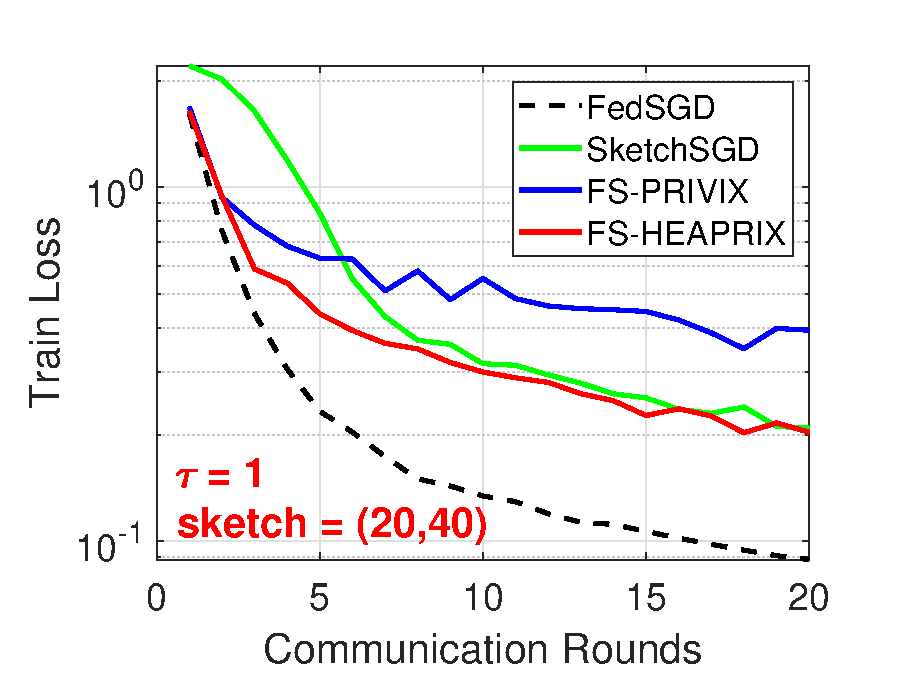
\includegraphics[width=1.7in]{MNIST_figures/local1_sketch20_iid1_train_loss.eps} \hspace{-0.12in}
		 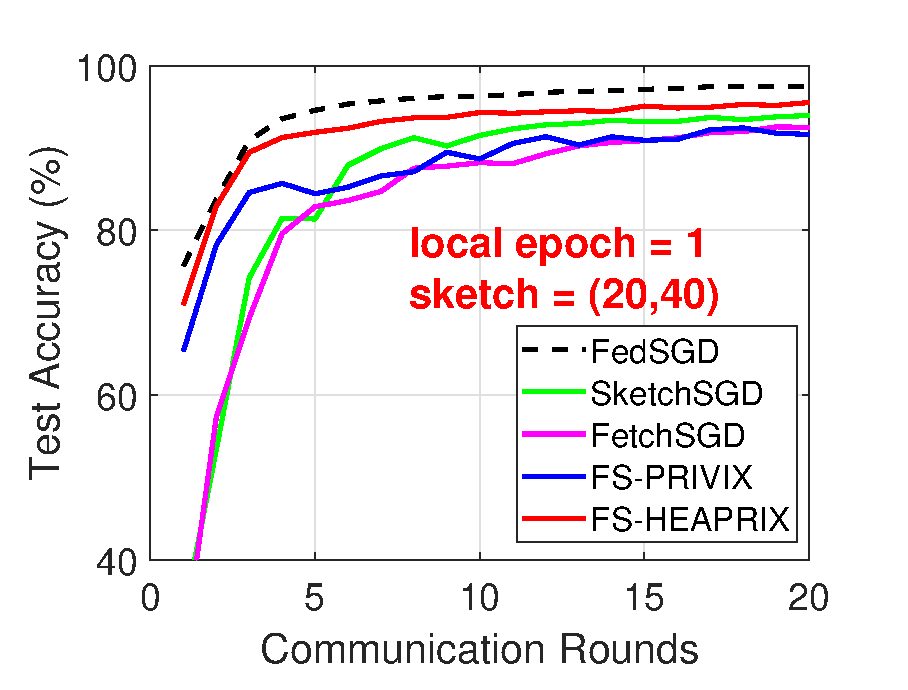
\includegraphics[width=1.7in]{MNIST_figures/local1_sketch20_iid1_test_acc.eps} 
		 }
		\mbox{\hspace{-0.15in}	
		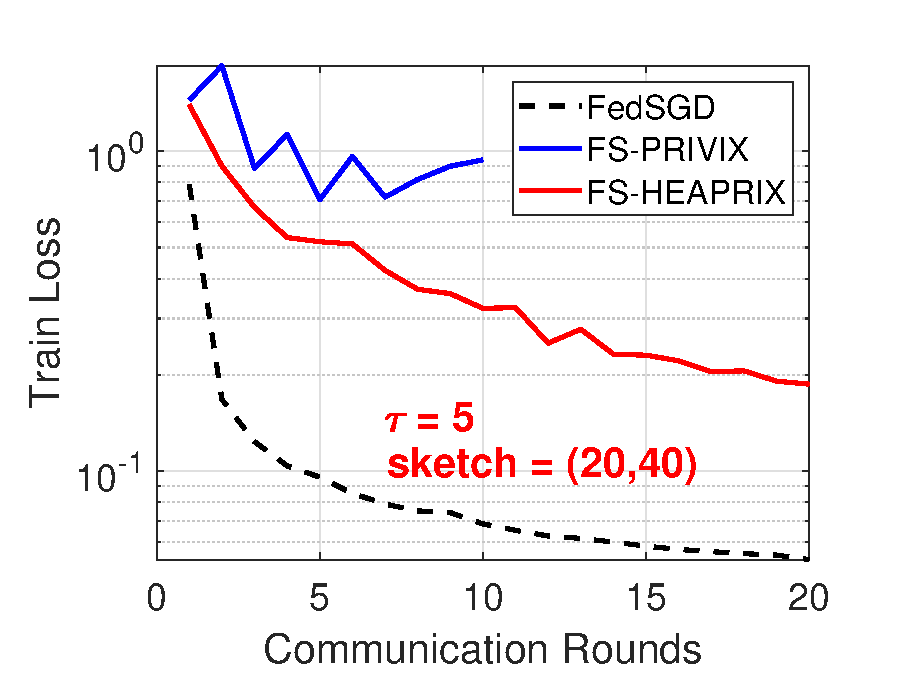
\includegraphics[width=1.7in]{MNIST_figures/local5_sketch20_iid1_train_loss.eps}\hspace{-0.12in}
		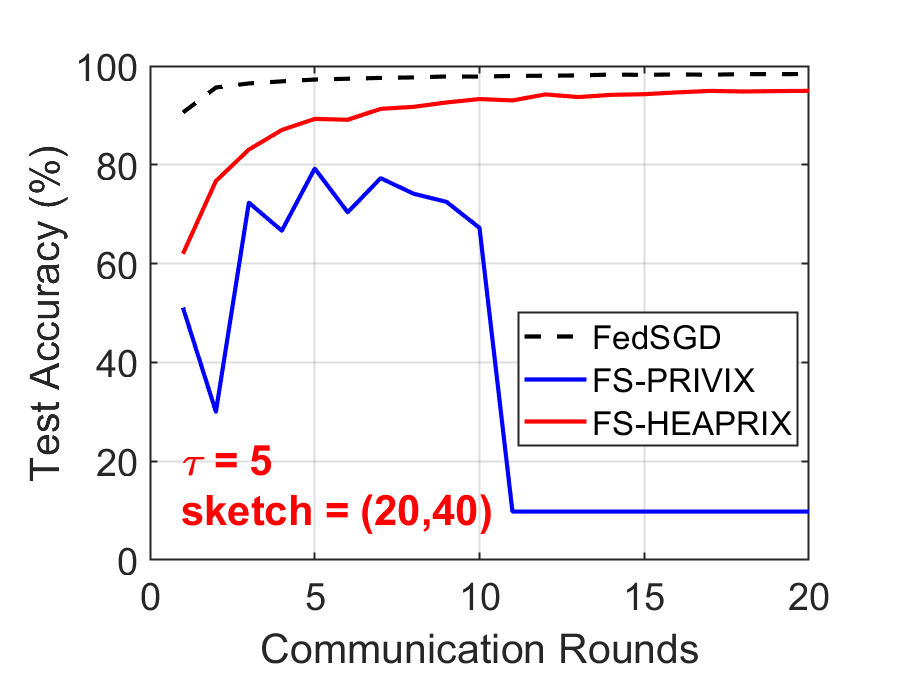
\includegraphics[width=1.7in]{MNIST_figures/local5_sketch20_iid1_test_acc.eps}
		}
		\mbox{\hspace{-0.15in}	
		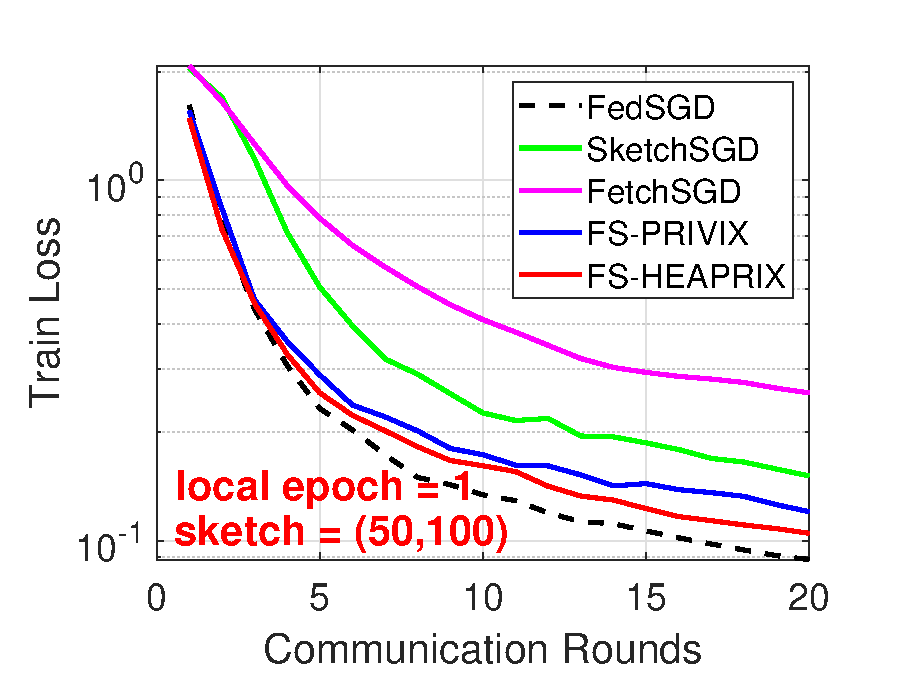
\includegraphics[width=1.7in]{MNIST_figures/local1_sketch50_iid1_train_loss.eps} \hspace{-0.12in}
		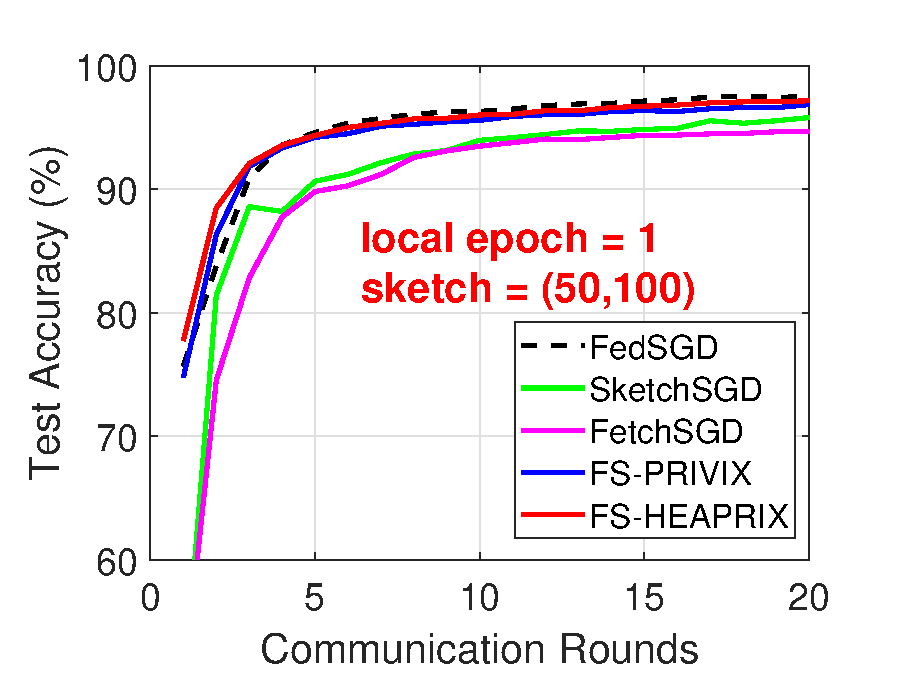
\includegraphics[width=1.7in]{MNIST_figures/local1_sketch50_iid1_test_acc.eps} 
		}
		\mbox{\hspace{-0.15in}	
		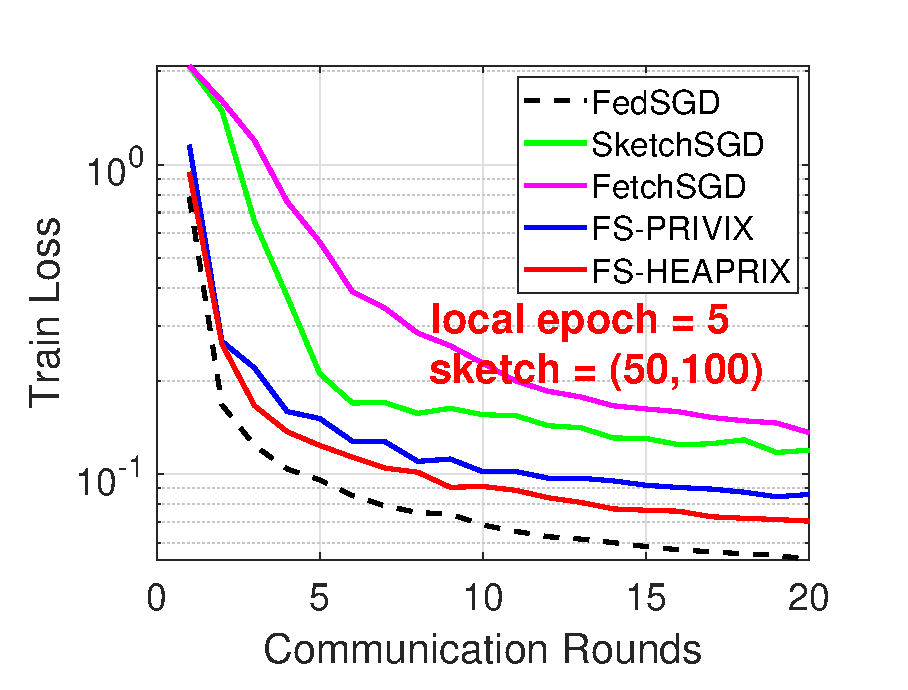
\includegraphics[width=1.7in]{MNIST_figures/local5_sketch50_iid1_train_loss.eps}\hspace{-0.12in}
		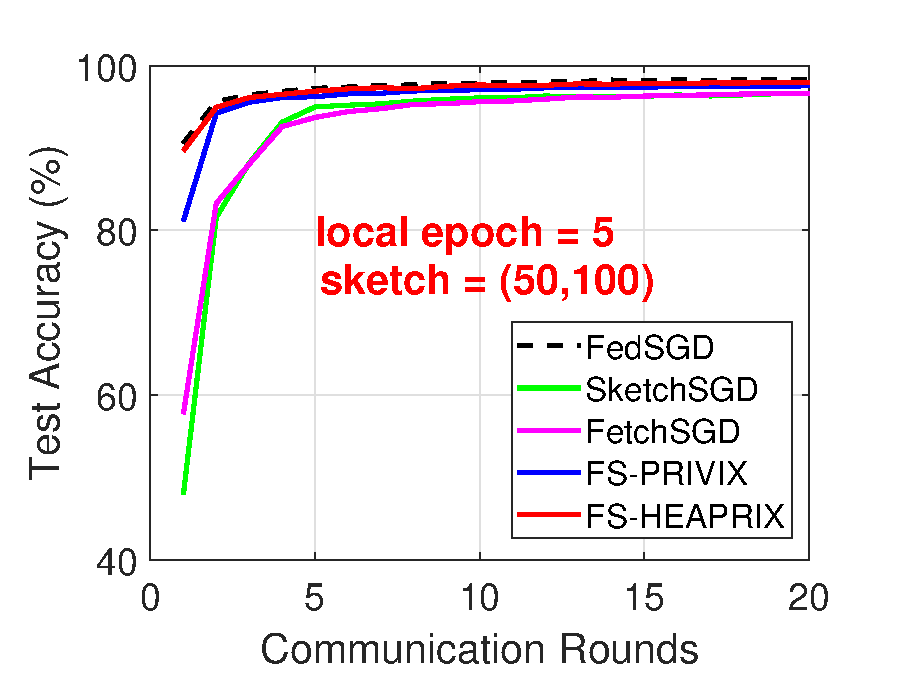
\includegraphics[width=1.7in]{MNIST_figures/local5_sketch50_iid1_test_acc.eps}
		}
	\end{center}
	\vspace{-0.1in}
	\caption{Homogeneous case: Comparison of compressed optimization methods on LeNet CNN.}
    \label{fig:MNIST-iid1}
    \vspace{-0.1in}
\end{figure}

\textbf{Homogeneous case.} In Figure~\ref{fig:MNIST-iid1}, we provide the training loss and test accuracy with different number of local epochs and sketch size, $(t,k)=(20,40)$ and $(50,100)$. 
Note that, these two choices of sketch size correspond to a $75\times$ and $12\times$ compression ratio, respectively. We conclude
\begin{itemize}
    \item In general, increasing compression ratio would sacrifice learning performance. In all cases, \texttt{FS-HEAPRIX} performs the best in terms of both training objective and test accuracy, among all compressed methods.
    
    \item \texttt{FS-HEAPRIX} is better than \texttt{FS-PRIVIX}, especially with small sketches (high compression ratio). \texttt{FS-HEAPRIX} yields acceptable extra test error compared to full-precision \texttt{FedSGD}, particularly when considering the high compression ratio (e.g., $75\times$). 
    
    \item From the training loss, we see that the performance of \texttt{FS-HEAPRIX} improves when the number of local updates increases. \emph{That is, the proposed method is able to further reduce the communication cost by reducing the number of rounds required for communication.} This is also consistent with our theoretical findings. 
\end{itemize}
In general, our proposed \texttt{FS-HEAPRIX} outperforms all competing methods, and a sketch size of $(50,100)$ is sufficient to approach the accuracy of full-precision \texttt{FedSGD}.

\begin{figure}[t]
	\begin{center}
		\mbox{\hspace{-0.1in}			   
		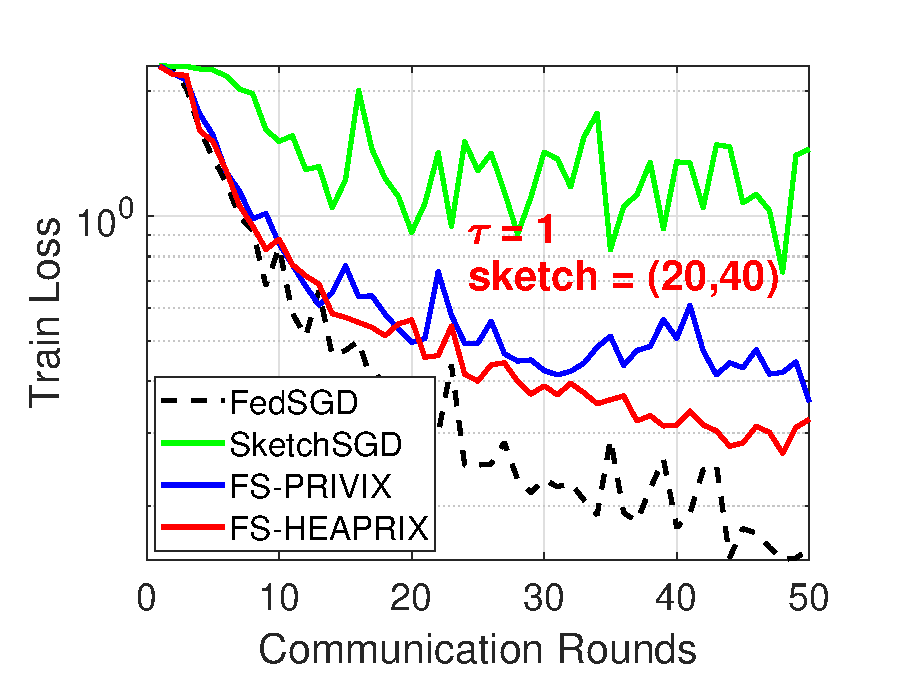
\includegraphics[width=1.7in]{MNIST_figures/local1_sketch20_iid0_train_loss.eps} \hspace{-0.12in}
		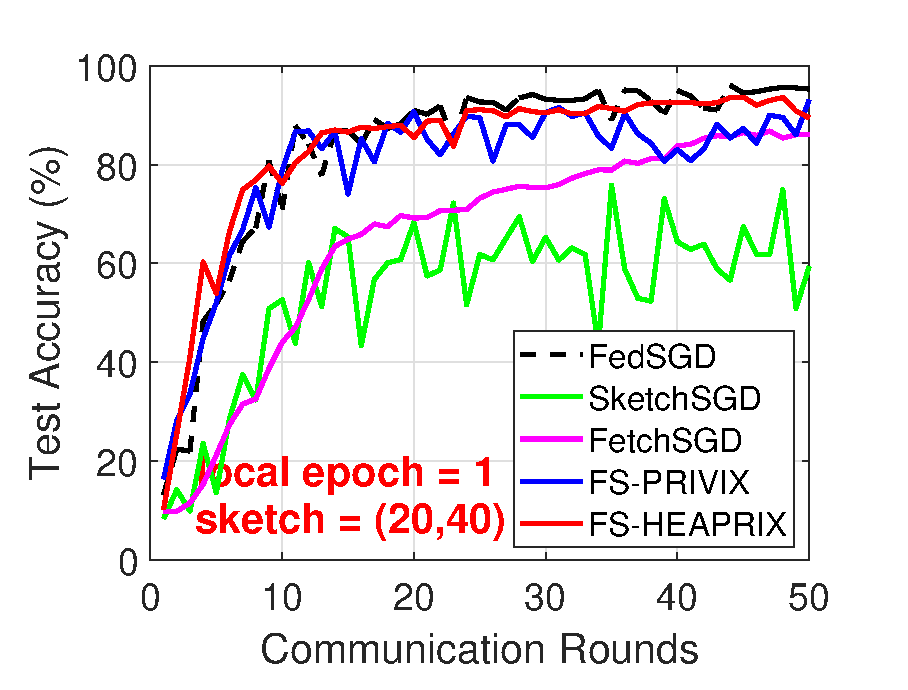
\includegraphics[width=1.7in]{MNIST_figures/local1_sketch20_iid0_test_acc.eps} 
		}
		\mbox{\hspace{-0.15in}	
		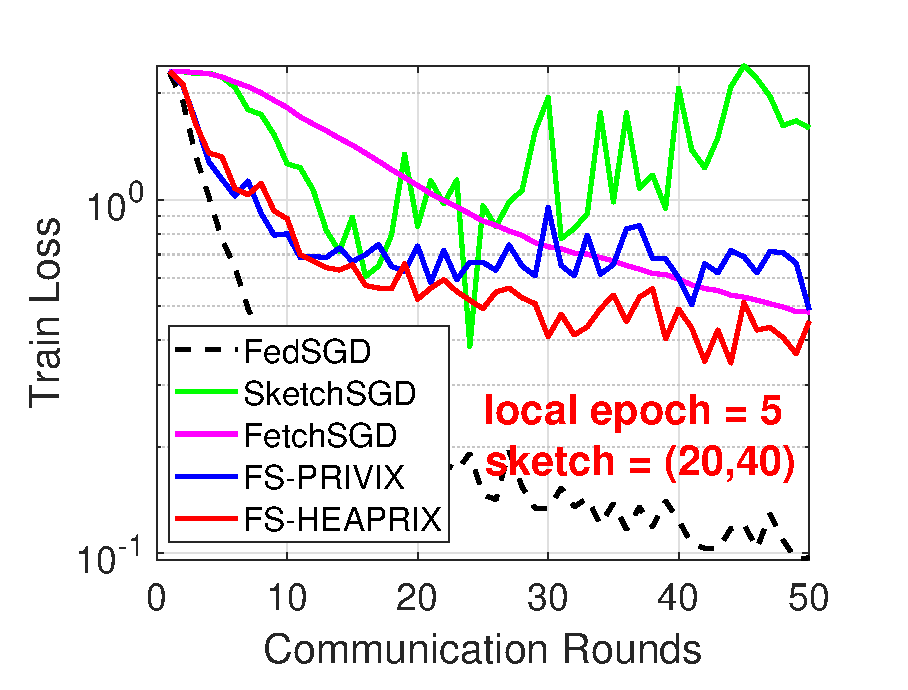
\includegraphics[width=1.7in]{MNIST_figures/local5_sketch20_iid0_train_loss.eps} \hspace{-0.12in}
		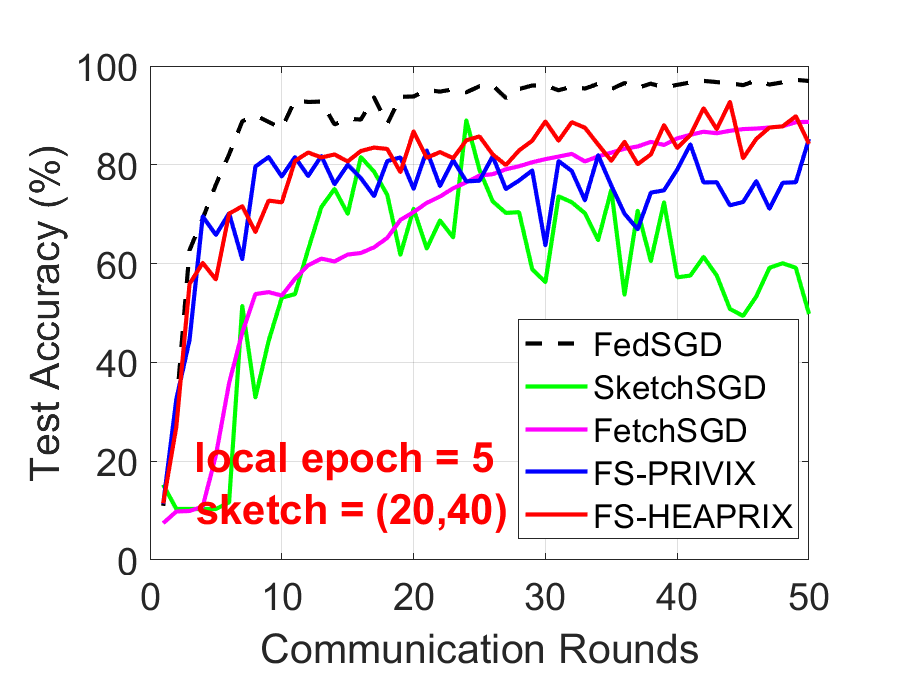
\includegraphics[width=1.7in]{MNIST_figures/local5_sketch20_iid0_test_acc.eps}
		}
		\mbox{\hspace{-0.15in}	
		 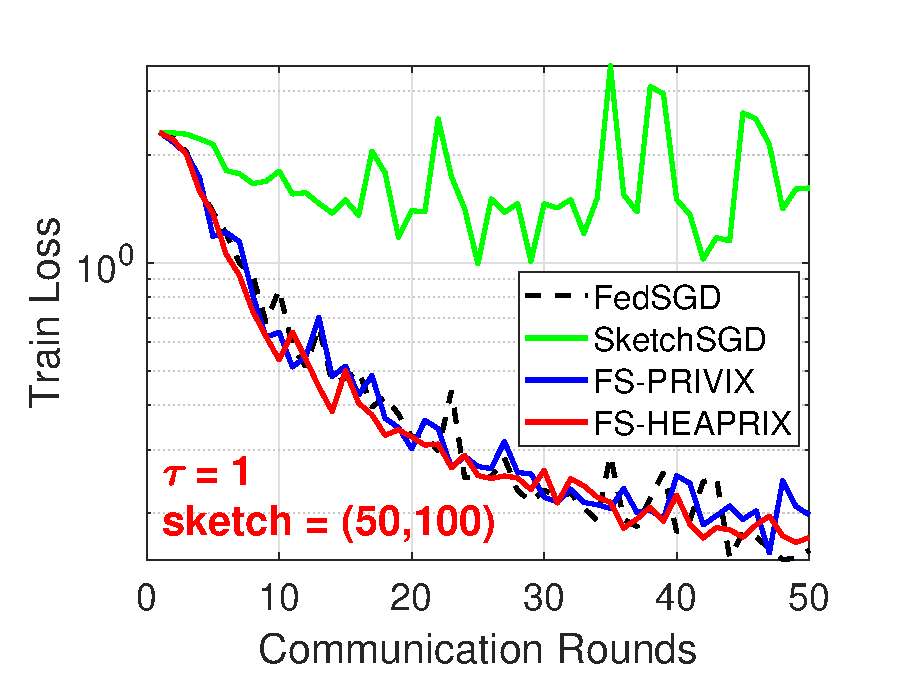
\includegraphics[width=1.7in]{MNIST_figures/local1_sketch50_iid0_train_loss.eps} \hspace{-0.12in}
		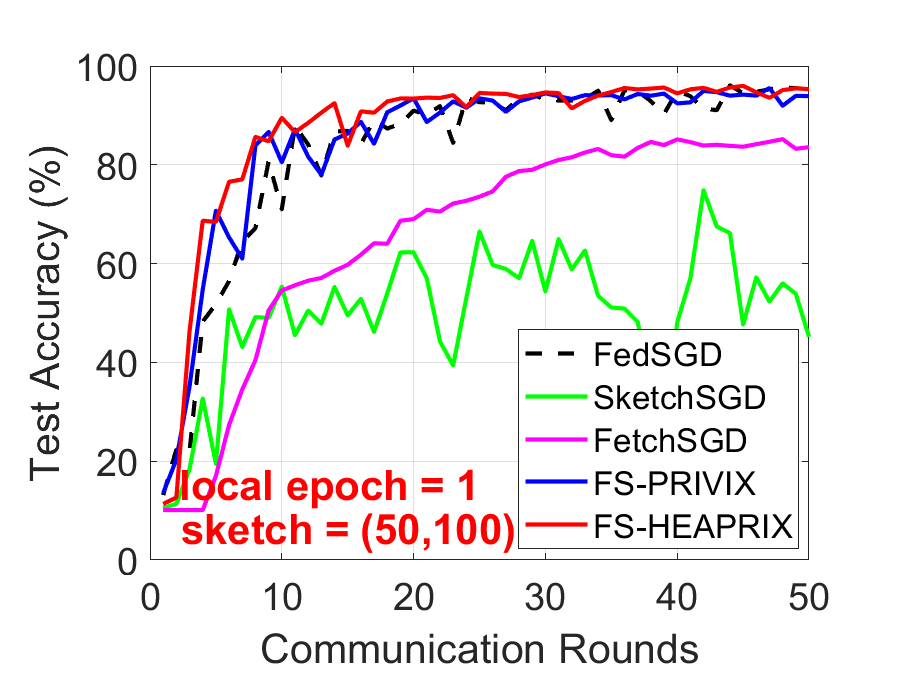
\includegraphics[width=1.7in]{MNIST_figures/local1_sketch50_iid0_test_acc.eps} 
		}
		\mbox{\hspace{-0.15in}	
		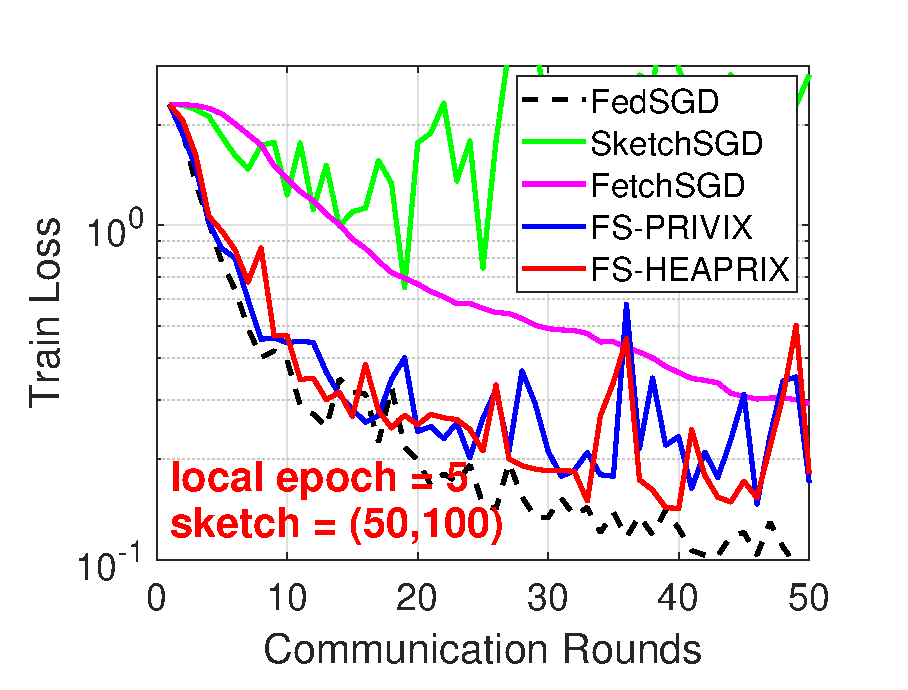
\includegraphics[width=1.7in]{MNIST_figures/local5_sketch50_iid0_train_loss.eps}\hspace{-0.12in}
		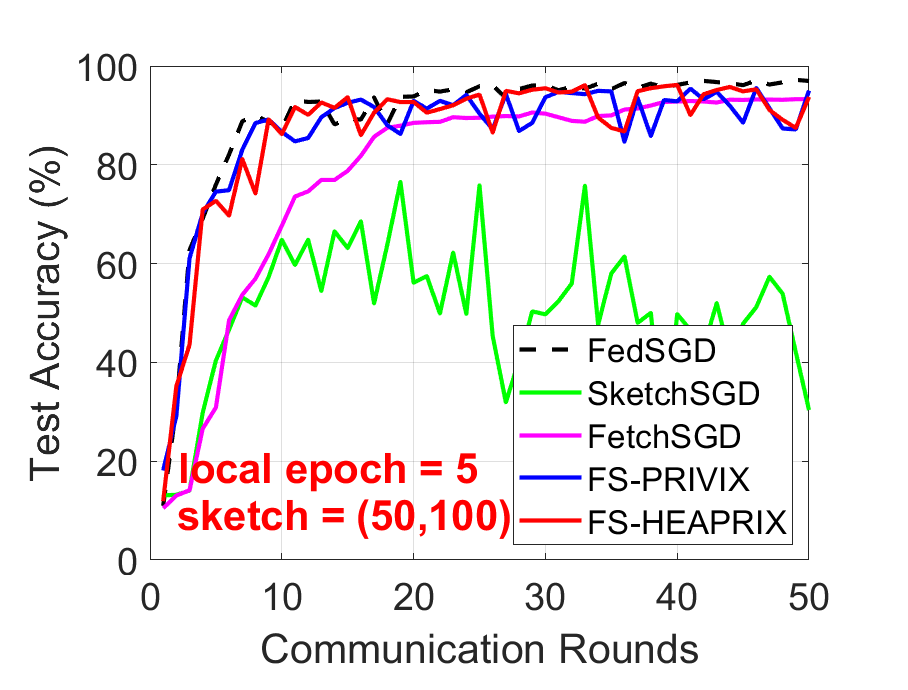
\includegraphics[width=1.7in]{MNIST_figures/local5_sketch50_iid0_test_acc.eps}
		}
	\end{center}
	\vspace{-0.1in}
	\caption{Heterogeneous case: Comparison of compressed optimization algorithms on LeNet CNN.}
    \label{fig:MNIST-iid0}
    \vspace{-0.1in}
\end{figure}

\textbf{Heterogeneous case.} We plot similar set of results in Figure~\ref{fig:MNIST-iid0} for non-i.i.d. data distribution, which leads to more twists and turns in the training curves. 
We see that \texttt{SketchSGD} performs very poorly in the heterogeneous case, which is improved by error tracking and momentum in \texttt{FetchSGD}, as expected. However, both of these methods are worse than our proposed \texttt{FedSketchGATE} methods, which can achieve similar generalization accuracy as full-precision \texttt{FedSGD}, even with small sketch size (i.e., $75\times$ compression with 1 local epoch). 
Note that, slower convergence and worse generalization of \texttt{FedSGD} in non-i.i.d. data distribution case is also reported in e.g.~\citet{mcmahan2016communication,chen2020toward}. 

We also notice in Figure~\ref{fig:MNIST-iid0} the advantage of \texttt{FS-HEAPRIX} over \texttt{FS-PRIVIX} in terms of training loss and test accuracy. 
However, empirically we see that in the heterogeneous setting, more local updates tend to undermine the learning performance, especially with small sketch size.  
Nevertheless, when the sketch size is not too small, i.e., $(50,100)$, \texttt{FS-HEAPRIX} can still provide comparable test accuracy as \texttt{FedSGD} in both cases.
Our empirical study demonstrates that our proposed \texttt{FedSketch} (and \texttt{FedSketchGATE}) frameworks are able to perform well in homogeneous (resp. heterogeneous) setting, with high compression rate. 
In particular, \texttt{FedSketch} methods are advantageous over recent \texttt{SketchedSGD}~\citep{ivkin2019communication} and \texttt{FetchSGD}~\cite{rothchild2020fetchsgd} in all cases. 
\texttt{FS-HEAPRIX} performs the best among all the tested compressed optimization algorithms, which in many cases achieves similar generalization accuracy as full-precision FedSGD with small sketch size. 

\vspace{-0.1in}
\section{Conclusion}
\vspace{-0.05in}

In this paper, we introduced \texttt{FedSKETCH} and \texttt{FedSKETCHGATE} algorithms for homogeneous and heterogeneous data distribution setting respectively for Federated Learning wherein communication between server and devices is only performed using count sketch. 
Our algorithms, thus, provide communication-efficiency and privacy, through random hashes based sketches. 
We analyze the convergence error for \emph{non-convex}, \emph{PL} and \emph{general convex} objective functions in the scope of Federated Optimization.  
We provide insightful numerical experiments showcasing the advantages of our \texttt{FedSKETCH} and \texttt{FedSKETCHGATE} methods over current federated optimization algorithm. The proposed algorithms outperform competing compression method and can achieve comparable test accuracy as Federated SGD, with high compression ratio.


\clearpage
\bibliographystyle{plainnat}
\bibliography{reference}
%%%%%%%%%%%%%%%%%%%%%%%%%%%%%%%%%%%%%%%%%%%%%%%%%%%%
\clearpage

\appendix
%\section{Appendix}
\section{Proof of main Theorems}
\subsection{Proof of Theorem~\ref{thm:homog_case}}

\subsection{Proof of Theorem~\ref{thm:hetreg_case}}
The following Lemma will be useful in our proof. 
\begin{lemma}
If you define $Q\triangleq3\sqrt[3]{\frac{ad^2}{2}}\sqrt{1+\sqrt{1+\frac{256 a}{27e^3d^4}}}$ and $$x\leq -\frac{1}{2}\sqrt{\frac{1}{3a}\left(Q-\frac{12a}{eQ}\right)}+\frac{1}{2}\sqrt{\frac{4}{eQ}-\frac{Q}{3a}+\frac{2d\sqrt{3}}{\sqrt{a}\sqrt{Q-\frac{12a}{e Q}}}}$$ then for positive constants $a,d,c\geq 0$, we have:
\begin{align}
    ax^{4}+dx-\frac{1}{e}\leq 0
\end{align}
\end{lemma}
\begin{proof}
We use the results in \cite{wiki:xxx} with $b=c=0$ and $p=0, q=\frac{d}{a}$. In this case, the only real valued root is 
\begin{align}
x&=-S+\frac{1}{2}\sqrt{-4S^2+\frac{d}{aS}},\:\text{and}\:S=\frac{1}{2}\sqrt{\frac{1}{3a}\left(Q-\frac{12a}{eQ}\right)}\nonumber\\
\implies x&=-\frac{1}{2}\sqrt{\frac{1}{3a}\left(Q-\frac{12a}{eQ}\right)}+\frac{1}{2}\sqrt{\frac{4}{eQ}-\frac{Q}{3a}+\frac{2d\sqrt{3}}{\sqrt{a}\sqrt{Q-\frac{12a}{e Q}}}} \nonumber\\
Q&=\sqrt[3]{\frac{{27a}{d^2}+\sqrt{\left({27a}{d^2}\right)^2+4\left(\frac{12a}{e}\right)^3}}{2}}=3\sqrt[3]{\frac{ad^2}{2}}\sqrt{1+\sqrt{1+\frac{256 a}{27e^3d^4}}}
\end{align} 
Therefore, we have with $Q=3\sqrt[3]{\frac{ad^2}{2}}\sqrt{1+\sqrt{1+\frac{256 a}{27e^3d^4}}}$:
\begin{align}
    x\leq -\frac{1}{2}\sqrt{\frac{1}{3a}\left(Q-\frac{12a}{eQ}\right)}+\frac{1}{2}\sqrt{\frac{4}{eQ}-\frac{Q}{3a}+\frac{2d\sqrt{3}}{\sqrt{a}\sqrt{Q-\frac{12a}{e Q}}}}
\end{align}
\end{proof}

Next, consider the following condition in~\cite{haddadpour2020federated}: 
\begin{align}
    \left(10\gamma^2L^4\tau^4\right)\eta^4+\left(L\gamma\tau\right)\eta-\frac{1}{q+1}\leq 0
\end{align}
where $a=10\gamma^2L^4\tau^4, d=L\gamma\tau$ and $e=q+1$, in this case 
\begin{align}
    Q=3\sqrt[3]{\frac{10}{2}}\gamma^{\frac{4}{3}} L^2\tau^2\underbrace{\sqrt{1+\sqrt{1+\frac{2560}{27\gamma^2(q+1)^3}}}}_{\triangleq C}=3\sqrt[3]{\frac{10}{2}}\gamma^{\frac{4}{3}} L^2\tau^2 C
\end{align}

Then we have:
\begin{align}
    x&\leq -\frac{1}{2}\sqrt{\frac{1}{3a}\left(Q-\frac{12a}{eQ}\right)}+\frac{1}{2}\sqrt{\frac{4}{eQ}-\frac{Q}{3a}+\frac{2d\sqrt{3}}{\sqrt{a}\sqrt{Q-\frac{12a}{e Q}}}}\nonumber\\
    &=-\frac{1}{2}\sqrt{\frac{3\sqrt[3]{\frac{10}{2}}\gamma^{\frac{4}{3}} L^2\tau^2 C}{30\gamma^2L^4\tau^4}-\frac{4}{(q+1)3\sqrt[3]{\frac{10}{2}}\gamma^{\frac{4}{3}} L^2\tau^2 C}}\nonumber\\
    &\quad+\frac{1}{2}\sqrt{\frac{4}{(q+1)3\sqrt[3]{\frac{10}{2}}\gamma^{\frac{4}{3}} L^2\tau^2 C}-\frac{3\sqrt[3]{\frac{10}{2}}\gamma^{\frac{4}{3}} L^2\tau^2 C}{30\gamma^2L^4\tau^4}+\frac{2L\gamma\tau\sqrt{3}}{\sqrt{10\gamma^2L^4\tau^4}\sqrt{3\sqrt[3]{\frac{10}{2}}\gamma^{\frac{4}{3}} L^2\tau^2 C-\frac{120 \gamma^2L^4\tau^4}{(q+1) 3\sqrt[3]{\frac{10}{2}}\gamma^{\frac{4}{3}} L^2\tau^2 C}}}}\nonumber\\
    &=\frac{1}{2L\tau\gamma^{\frac{1}{3}}}\Big(\sqrt{\frac{4}{(q+1)3\sqrt[3]{\frac{10}{2}}\gamma^{\frac{2}{3}} C}-\frac{\sqrt[3]{\frac{10}{2}} C}{10}+\frac{2\sqrt{3}}{\sqrt{10}\sqrt{3\sqrt[3]{\frac{10}{2}} C-\frac{40 }{(q+1)\gamma^{\frac{2}{3}} \sqrt[3]{\frac{10}{2}} C}}}}-\sqrt{\frac{\sqrt[3]{\frac{10}{2}} C}{10}-\frac{4}{(q+1)3\sqrt[3]{\frac{10}{2}}\gamma^{\frac{2}{3}} C}}\Big)\nonumber\\
\end{align}
%%%%%%%%%%%%%%%%%%%%%%%%%%%%%%%%%%%%%%%%%%%%%%%%
%%%%%%%%%%%%%%%%%%%%%%%%%%%%%%%%%%%%%%%%%%%%%%%%
\section{Convergence result for \texttt{FEDSKETCH} without memory}
From the $L$-smoothness gradient assumption on global objective, by using  $\underline{\mathbf{S}}^{(r)}=\tilde{\mathbf{g}}^{(r)}$ in inequality (\ref{eq:decent-smoothe}) we have:
\begin{align}
    f({\boldsymbol{x}}^{(r+1)})-f({\boldsymbol{x}}^{(r)})\leq -\gamma \big\langle\nabla f({\boldsymbol{x}}^{(r)}),\tilde{\mathbf{g}}^{(r)}\big\rangle+\frac{\gamma^2 L}{2}\|\tilde{\mathbf{g}}^{(r)}\|^2\label{eq:Lipschitz-c1}
\end{align}
We define the following:
\begin{align}
    \tilde{\mathbf{g}}_{\mathbf{S}}^{(r)}=\frac{\eta}{p}\sum_{j=1}^{p}\mathbf{S}\left[\sum_{c=0}^{\tau-1}\tilde{\mathbf{g}}_j^{(c,r)}\right]
\end{align}
Additionally, we define an auxiliary variable as 
\begin{align}
    \tilde{\mathbf{g}}^{(r)}=\frac{\eta}{p}\sum_{j=1}^{p}\left[\sum_{c=0}^{\tau-1}\tilde{\mathbf{g}}_j^{(c,r)}\right]
\end{align}
%%%%%%%%%%%%%%%%%%%%%%%%%%%%%%%%%%%%%%%%%%%%
By taking expectation on both sides of above inequality over sampling, we get:
\begin{align}
    \mathbb{E}\left[\mathbb{E}_\mathbf{S}\Big[f({\boldsymbol{x}}^{(r+1)})-f({\boldsymbol{x}}^{(r)})\Big]\right]&\leq -\gamma\mathbb{E}\left[\mathbb{E}_\mathbf{S}\left[ \big\langle\nabla f({\boldsymbol{x}}^{(r)}),\tilde{\mathbf{g}}_\mathbf{S}^{(r)}\big\rangle\right]\right]+\frac{\gamma^2 L}{2}\mathbb{E}\left[\mathbb{E}_\mathbf{S}\|\tilde{\mathbf{g}}_\mathbf{S}^{(r)}\|^2\right]\nonumber\\
    &=-\gamma\mathbb{E}\left[\mathbb{E}_\mathbf{S}\left[ \big\langle\nabla f({\boldsymbol{x}}^{(r)}),\tilde{\mathbf{g}}^{(r)}\big\rangle\right]\right]+\gamma\mathbb{E}\left[\mathbb{E}_\mathbf{S}\left[ \big\langle\nabla f({\boldsymbol{x}}^{(r)}),\tilde{\mathbf{g}}^{(r)}-\tilde{\mathbf{g}}_{\mathbf{S}}^{(r)}\big\rangle\right]\right]\nonumber\\
    &\qquad+\frac{\gamma^2 L}{2}\mathbb{E}\left[\mathbb{E}_\mathbf{S}\|\tilde{\mathbf{g}}_\mathbf{S}^{(r)}-\tilde{\mathbf{g}}^{(r)}+\tilde{\mathbf{g}}^{(r)}\|^2\right] \nonumber\\
    &\stackrel{(a)}{=}-\gamma\mathbb{E}\left[\mathbb{E}_\mathbf{S}\left[ \big\langle\nabla f({\boldsymbol{x}}^{(r)}),\tilde{\mathbf{g}}^{(r)}\big\rangle\right]\right]+\gamma\left[\mathbb{E}_\mathbf{S}\left[ \big\langle\nabla f({\boldsymbol{x}}^{(r)}),{\mathbf{g}}^{(r)}-{\mathbf{g}}_{\mathbf{S}}^{(r)}\big\rangle\right]\right]\nonumber\\
    &\qquad+\frac{\gamma^2 L}{2}\mathbb{E}\left[\mathbb{E}_\mathbf{S}\|\tilde{\mathbf{g}}_\mathbf{S}^{(r)}-\tilde{\mathbf{g}}^{(r)}+\tilde{\mathbf{g}}^{(r)}\|^2\right]\nonumber\\
    &\stackrel{(b)}{\leq}-\gamma\mathbb{E}\left[\mathbb{E}_\mathbf{S}\left[ \big\langle\nabla f({\boldsymbol{x}}^{(r)}),\tilde{\mathbf{g}}^{(r)}\big\rangle\right]\right]+\frac{\gamma}{2}\left[ \frac{1}{mL}\left\|\nabla f({\boldsymbol{x}}^{(r)})\right\|^2_2+mL\mathbb{E}_\mathbf{S}\left[\left\|{\mathbf{g}}^{(r)}-{\mathbf{g}}_{\mathbf{S}}^{(r)}\right\|^2_2\right]\right]\nonumber\\
    &\qquad+{\gamma^2 L}\mathbb{E}\left[\mathbb{E}_\mathbf{S}\left\|\tilde{\mathbf{g}}_\mathbf{S}^{(r)}-\tilde{\mathbf{g}}^{(r)}\right\|+\left\|\tilde{\mathbf{g}}^{(r)}\right\|^2\right] \nonumber\\
    &\stackrel{(c)}{\leq}-\gamma\mathbb{E}\left[ \big\langle\nabla f({\boldsymbol{x}}^{(r)}),\tilde{\mathbf{g}}^{(r)}\big\rangle\right]+\frac{\gamma}{2}\left[ \frac{1}{mL}\left\|\nabla f({\boldsymbol{x}}^{(r)})\right\|^2_2+mL\left(1-\frac{k}{d}\right)\left\|{\mathbf{g}}^{(r)}\right\|^2_2\right]\nonumber\\
    &\qquad+{\gamma^2 L}\mathbb{E}\left[\left(1-\frac{k}{d}\right)\left\|\tilde{\mathbf{g}}^{(r)}\right\|_2^2+\left\|\tilde{\mathbf{g}}^{(r)}\right\|_2^2\right]\nonumber\\
    &\stackrel{(d)}{=}-\gamma\underbrace{\mathbb{E}\left[ \big\langle\nabla f({\boldsymbol{x}}^{(r)}),\tilde{\mathbf{g}}^{(r)}\big\rangle\right]}_{(\mathrm{I})}+ \frac{\gamma}{2mL}\left\|\nabla f({\boldsymbol{x}}^{(r)})\right\|^2_2+\frac{mL\gamma}{2}\left(1-\frac{k}{d}\right)\underbrace{\left\|{\mathbf{g}}^{(r)}\right\|^2_2}_{(\mathrm{II})}\nonumber\\
    &\qquad+{\gamma^2 L}\left(2-\frac{k}{d}\right)\underbrace{\mathbb{E}\left[\left\|\tilde{\mathbf{g}}^{(r)}\right\|_2^2\right]}_{(\mathrm{III})}\label{eq:Lipschitz-c-gd-alt}
\end{align}
To bound term ($\mathrm{I}$) in Eq.~(\ref{eq:Lipschitz-c-gd-alt}) we use the combination of Lemmas~\ref{} and \ref{} we obtain:
\begin{align}
    -\gamma\mathbb{E}\left[ \big\langle\nabla f({\boldsymbol{x}}^{(r)}),\tilde{\mathbf{g}}^{(r)}\big\rangle\right]\leq \frac{\gamma}{2}\eta\frac{1}{p}\sum_{j=1}^p\sum_{c=0}^{\tau-1}\left[-\left\|\nabla f({\boldsymbol{x}}^{(r)})\right\|_2^2-\left\|\mathbf{g}_j^{(\ell,r)}\right\|_2^2+L^2\eta^2\sum_{\ell=0}^{\tau-1}\left[\tau\left\|{\mathbf{g}}_j^{(\ell,r)}\right\|_2^2+\sigma^2\right]\right]
\end{align}
Term $(\mathrm{II})$ can be bounded simply as follows:
\begin{align}
    \left\|{\mathbf{g}}^{(r)}\right\|^2_2&=\left\|\frac{\eta}{p}\sum_{j=1}^{p}\left[\sum_{c=0}^{\tau-1}{\mathbf{g}}_j^{(c,r)}\right]\right\|^2_2\nonumber\\
    &\leq\frac{\tau\eta^2}{p}\sum_{j=1}^{p}\sum_{c=0}^{\tau-1}\left\|\mathbf{g}_j^{(c,r)}\right\|^2_2
\end{align}

Next we bound term $(\mathrm{III})$ using the following lemma:
\begin{lemma}
\begin{align}
    \mathbb{E}\left[\left\|\tilde{\mathbf{g}}^{(r)}\right\|_2^2\right]\leq \frac{\eta^2\tau}{p}\sum_{j=1}^{p}\sum_{c=0}^{\tau-1}\left\|\mathbf{g}_j^{(c,r)}\right\|^2_2+\frac{\eta^2\tau}{p}\sigma^2
\end{align}
\end{lemma}
\begin{proof}
\begin{align}
    \mathbb{E}\left[\left\|\tilde{\mathbf{g}}^{(r)}\right\|_2^2\right]&=\mathbb{E}\left[\left\|\tilde{\mathbf{g}}^{(r)}-\mathbb{E}\left[\tilde{\mathbf{g}}^{(r)}\right]\right\|_2^2\right]+\left\|\mathbb{E}\left[\tilde{\mathbf{g}}^{(r)}\right]\right\|^2_2\nonumber\\
    &= \mathbb{E}\left[\left\|\tilde{\mathbf{g}}^{(r)}-{\mathbf{g}}^{(r)}\right\|_2^2\right]+\left\|{\mathbf{g}}^{(r)}\right\|^2_2\nonumber\\
    &= \mathbb{E}\left[\left\|\frac{\eta}{p}\sum_{j=1}^{p}\left[\sum_{c=0}^{\tau-1}\tilde{\mathbf{g}}_j^{(c,r)}\right]-\frac{\eta}{p}\sum_{j=1}^{p}\left[\sum_{c=0}^{\tau-1}\mathbf{g}_j^{(c,r)}\right]\right\|_2^2\right]+\left\|\frac{\eta}{p}\sum_{j=1}^{p}\left[\sum_{c=0}^{\tau-1}\mathbf{g}_j^{(c,r)}\right]\right\|^2_2\nonumber\\
&=\frac{\eta^2}{p^2}\sum_{j=1}^{p}\sum_{c=0}^{\tau-1}\mathbb{E}\left[\left\|\tilde{\mathbf{g}}_j^{(c,r)}-\mathbf{g}_j^{(c,r)}\right\|_2^2\right]+\left\|\frac{\eta}{p}\sum_{j=1}^{p}\left[\sum_{c=0}^{\tau-1}\mathbf{g}_j^{(c,r)}\right]\right\|^2_2 \nonumber\\
&\leq \frac{\eta^2}{p^2}\sum_{j=1}^{p}\sum_{c=0}^{\tau-1}\mathbb{E}\left[\left\|\tilde{\mathbf{g}}_j^{(c,r)}-\mathbf{g}_j^{(c,r)}\right\|_2^2\right]+\frac{\eta^2\tau}{p}\sum_{j=1}^{p}\sum_{c=0}^{\tau-1}\left\|\mathbf{g}_j^{(c,r)}\right\|^2_2\nonumber\\
&\leq \frac{\eta^2}{p^2}\sum_{j=1}^{p}\sum_{c=0}^{\tau-1}\sigma^2+\frac{\eta^2\tau}{p}\sum_{j=1}^{p}\sum_{c=0}^{\tau-1}\left\|\mathbf{g}_j^{(c,r)}\right\|^2_2\nonumber\\
&=\frac{\eta^2\tau}{p}\sum_{j=1}^{p}\sum_{c=0}^{\tau-1}\left\|\mathbf{g}_j^{(c,r)}\right\|^2_2+\frac{\eta^2\tau}{p}\sigma^2
\end{align}
\end{proof}
Next, we put all the pieces together as follows:
\begin{align}
    \mathbb{E}\left[\mathbb{E}_\mathbf{S}\Big[f({\boldsymbol{x}}^{(r+1)})-f({\boldsymbol{x}}^{(r)})\Big]\right]&\leq \frac{\gamma}{2}\eta\frac{1}{p}\sum_{j=1}^p\sum_{\ell=0}^{\tau-1}\left[-\left\|\nabla f({\boldsymbol{x}}^{(r)})\right\|_2^2-\left\|\mathbf{g}_j^{(\ell,r)}\right\|_2^2+L^2\eta^2\sum_{\ell=0}^{\tau-1}\left[\tau\left\|{\mathbf{g}}_j^{(\ell,r)}\right\|_2^2+\sigma^2\right]\right]\nonumber\\
    &\quad+ \frac{\gamma}{2mL}\left\|\nabla f({\boldsymbol{x}}^{(r)})\right\|^2_2+\frac{mL\gamma}{2}\left(1-\frac{k}{d}\right)\frac{\tau\eta^2}{p}\sum_{j=1}^{p}\sum_{\ell=0}^{\tau-1}\left\|\mathbf{g}_j^{(\ell,r)}\right\|^2_2\nonumber\\
    &\quad+\gamma^2 L\left(2-\frac{k}{d}\right)\left[\frac{\eta^2\tau}{p}\sum_{j=1}^{p}\sum_{c=0}^{\tau-1}\left\|\mathbf{g}_j^{(\ell,r)}\right\|^2_2+\frac{\eta^2\tau}{p}\sigma^2\right]\nonumber\\
    &=-\frac{\tau\eta\gamma}{2}\left\|\nabla f({\boldsymbol{x}}^{(r)})\right\|_2^2+\frac{\gamma}{2}\eta\frac{1}{p}\sum_{j=1}^p\sum_{\ell=0}^{\tau-1}\left[-\left\|\mathbf{g}_j^{(\ell,r)}\right\|_2^2+L^2\eta^2\tau^2\left\|{\mathbf{g}}_j^{(\ell,r)}\right\|_2^2\right]+\frac{\gamma\eta^3L^2\tau^2}{2}\sigma^2\nonumber\\
    &\quad+ \frac{\gamma}{2mL}\left\|\nabla f({\boldsymbol{x}}^{(r)})\right\|^2_2+\frac{mL\gamma}{2}\left(1-\frac{k}{d}\right)\frac{\tau\eta^2}{p}\sum_{j=1}^{p}\sum_{\ell=0}^{\tau-1}\left\|\mathbf{g}_j^{(\ell,r)}\right\|^2_2\nonumber\\
    &\quad+\gamma^2 L\left(2-\frac{k}{d}\right)\frac{\eta^2\tau}{p}\sum_{j=1}^{p}\sum_{\ell=0}^{\tau-1}\left\|\mathbf{g}_j^{(\ell,r)}\right\|^2_2+\gamma^2 L\left(2-\frac{k}{d}\right)\frac{\eta^2\tau}{p}\sigma^2\nonumber\\
    &=-\left(\frac{\tau\eta\gamma}{2}-\frac{\gamma}{2mL}\right)\left\|\nabla f({\boldsymbol{x}}^{(r)})\right\|_2^2\nonumber\\
    &\quad-\left(\frac{\eta\gamma}{2}-\frac{\eta\gamma}{2}\left(L^2\eta^2\tau^2\right)-\frac{mL\eta\gamma}{2}\left(1-\frac{k}{d}\right)\tau\eta-\gamma^2 L\eta^2\tau\left(2-\frac{k}{d}\right)\right)\frac{1}{p}\sum_{j=1}^{p}\sum_{\ell=0}^{\tau-1}\left\|\mathbf{g}_j^{(\ell,r)}\right\|^2_2\nonumber\\
    &\quad+\frac{\gamma\eta^3L^2\tau^2}{2}\sigma^2+\gamma^2 L\left(2-\frac{k}{d}\right)\frac{\eta^2\tau}{p}\sigma^2\nonumber\\
    &\stackrel{(a)}{\leq}-\left(\frac{\tau\eta\gamma}{2}-\frac{\gamma}{2mL}\right)\left\|\nabla f({\boldsymbol{x}}^{(r)})\right\|_2^2+\frac{\gamma\eta^3L^2\tau^2}{2}\sigma^2+\tau\eta^2\gamma^2 L\left(2-\frac{k}{d}\right)\frac{\sigma^2}{p}\label{eq:ncvx-mid-step}
\end{align}
where (a) follows from the learning rate choices of 
\begin{align}
    \frac{\eta\gamma}{2}-\frac{\eta\gamma}{2}\left(L^2\eta^2\tau^2\right)-\frac{mL\eta\gamma}{2}\left(1-\frac{k}{d}\right)\tau\eta-\gamma^2 L\eta^2\tau\left(2-\frac{k}{d}\right)\geq 0
\end{align}
which can be simplified further as follows:
\begin{align}
    1-L^2\eta^2\tau^2-mL\tau\eta\left(1-\frac{k}{d}\right)-2\gamma L\eta\tau\left(2-\frac{k}{d}\right)\geq 0
\end{align}
Then using Eq.~(\ref{eq:ncvx-mid-step}) we obtain:
\begin{align}
  \frac{\tau\gamma}{2} \left({\eta}-\frac{1}{\tau mL}\right)\left\|\nabla f({\boldsymbol{x}}^{(r)})\right\|_2^2\leq \mathbb{E}\left[\mathbb{E}_\mathbf{S}\Big[f({\boldsymbol{x}}^{(r+1)})-f({\boldsymbol{x}}^{(r)})\Big]\right]+\tau\eta^2\gamma^2 L\left(2-\frac{k}{d}\right)\frac{\sigma^2}{p}+\frac{\gamma\eta^3L^2\tau^2}{2}\sigma^2
\end{align}
which leads to the following bound:
\begin{align}
     \left\|\nabla f({\boldsymbol{x}}^{(r)})\right\|_2^2\leq \frac{2 \mathbb{E}\left[\mathbb{E}_\mathbf{S}\Big[f({\boldsymbol{x}}^{(r+1)})-f({\boldsymbol{x}}^{(r)})\Big]\right]}{\tau \gamma \left({\eta}-\frac{1}{\tau mL}\right)}+\frac{2\eta^2\gamma L\left(2-\frac{k}{d}\right)\frac{\sigma^2}{p}}{ \left({\eta}-\frac{1}{\tau mL}\right)}+\frac{\eta^3L^2\tau}{\left({\eta}-\frac{1}{\tau mL}\right)}\sigma^2 
\end{align}
Now averaging over $r$ communication rounds we achieve:
\begin{align}
    \frac{1}{R}\sum_{r=0}^{R-1}\left\|\nabla f({\boldsymbol{x}}^{(r)})\right\|_2^2\leq \frac{2 \mathbb{E}\left[\mathbb{E}_\mathbf{S}\Big[f({\boldsymbol{x}}^{(0)})-f({\boldsymbol{x}}^{(*)})\Big]\right]}{R\tau \gamma \left({\eta}-\frac{1}{\tau mL}\right)}+\frac{2\eta^2\gamma L\left(2-\frac{k}{d}\right)\frac{\sigma^2}{p}}{ \left({\eta}-\frac{1}{\tau mL}\right)}+\frac{\eta^3L^2\tau}{\left({\eta}-\frac{1}{\tau mL}\right)}\sigma^2 
\end{align}
We note that for this case we have the following conditions over learning rate:
\begin{align}
    L^2\eta^2\tau^2+mL\tau\eta\left(1-\frac{k}{d}\right)+2\gamma L\eta\tau\left(2-\frac{k}{d}\right)\leq 1,\:\eta> \frac{1}{mL\tau},
\end{align}

\subsection{Proof of Theorem~\ref{thm:pl-iid}}
From Eq.~(\ref{eq:ncvx-mid-step}) under condition with:
\begin{align}
       L^2\eta^2\tau^2+mL\tau\eta\left(1-\frac{k}{d}\right)+2\gamma L\eta\tau\left(2-\frac{k}{d}\right)\leq 1, \label{eq:step_size_cnd_mmr}
\end{align}
we obtain:
\begin{align}
         \mathbb{E}\left[f({\boldsymbol{w}}^{(r+1)})-f({\boldsymbol{w}}^{(r)})\right]&\leq -\left(\frac{\tau\eta\gamma}{2}-\frac{\gamma}{2mL}\right)\left\|\nabla f({\boldsymbol{x}}^{(r)})\right\|_2^2+\frac{\gamma\eta^3L^2\tau^2}{2}\sigma^2+\tau\eta^2\gamma^2 L\left(2-\frac{k}{d}\right)\frac{\sigma^2}{p}\nonumber\\
         &\stackrel{(PL)}{\leq} -\left({\tau\mu\eta\gamma}-\frac{\mu\gamma}{mL}\right)\left[f({\boldsymbol{w}}^{(r)})-f({\boldsymbol{w}}^{(*)})\right]+\frac{\gamma\eta^3L^2\tau^2}{2}\sigma^2+\tau\eta^2\gamma^2 L\left(2-\frac{k}{d}\right)\frac{\sigma^2}{p} 
\end{align}
which leads to the following bound:
\begin{align}
            \mathbb{E}\Big[f({\boldsymbol{w}}^{(r+1)})-f({\boldsymbol{w}}^{(*)})\Big]&\leq \left(1-\eta\mu\gamma{\tau}+\frac{\mu\gamma}{mL}\right) \Big[f({\boldsymbol{w}}^{(r)})-f({\boldsymbol{w}}^{(*)})\Big]+\frac{\gamma\eta^3L^2\tau^2}{2}\sigma^2+\tau\eta^2\gamma^2 L\left(2-\frac{k}{d}\right)\frac{\sigma^2}{p} 
\end{align}
which leads to the following bound by setting $\Delta\triangleq1-\eta\mu\gamma{\tau}+\frac{\mu\gamma}{mL}=1-\mu\gamma\tau\left(\eta-\frac{1}{mL\tau}\right)$:
\begin{align}
            \mathbb{E}\Big[f({\boldsymbol{w}}^{(R)})-f({\boldsymbol{w}}^{(*)})\Big]&\leq \Delta^R \Big[f({\boldsymbol{w}}^{(0)})-f({\boldsymbol{w}}^{(*)})\Big]+\frac{1-\Delta^R}{1-\Delta}\left(\frac{\gamma\eta^3L^2\tau^2}{2}\sigma^2+\tau\eta^2\gamma^2 L\left(2-\frac{k}{d}\right)\frac{\sigma^2}{p} \right)\nonumber\\
            &\leq \Delta^R \Big[f({\boldsymbol{w}}^{(0)})-f({\boldsymbol{w}}^{(*)})\Big]+\frac{1}{1-\Delta}\left(\frac{\gamma\eta^3L^2\tau^2}{2}\sigma^2+\tau\eta^2\gamma^2 L\left(2-\frac{k}{d}\right)\frac{\sigma^2}{p} \right)\nonumber\\
            &={\left(1-\mu\gamma\tau\left(\eta-\frac{1}{mL\tau}\right)\right)}^R \Big[f({\boldsymbol{w}}^{(0)})-f({\boldsymbol{w}}^{(*)})\Big]+\frac{\left(\frac{\gamma\eta^3L^2\tau^2}{2}\sigma^2+\tau\eta^2\gamma^2 L\left(2-\frac{k}{d}\right)\frac{\sigma^2}{p} \right)}{\mu\gamma\tau\left(\eta-\frac{1}{m L\tau}\right)}\nonumber\\
            &\leq \exp{-\left(\mu\gamma\tau\left(\eta-\frac{1}{m L\tau}\right)R\right)}\Big[f({\boldsymbol{w}}^{(0)})-f({\boldsymbol{w}}^{(*)})\Big]+\frac{\left(\frac{\gamma\eta^3L^2\tau}{2}\sigma^2+\eta^2\gamma^2 L\left(2-\frac{k}{d}\right)\frac{\sigma^2}{p} \right)}{\mu\gamma\left(\eta-\frac{1}{mL\tau}\right)}
\end{align}
Then for the choice of $\eta=\frac{n}{mL\tau}$, for $m>n>1$, we obtain:


\begin{align}
                \mathbb{E}\Big[f({\boldsymbol{w}}^{(R)})-f({\boldsymbol{w}}^{(*)})\Big]&\leq \exp{-\left(\frac{\gamma\left(n-1\right) R}{m\kappa}\right) }\Big[f({\boldsymbol{w}}^{(0)})-f({\boldsymbol{w}}^{(*)})\Big]+\frac{\left(\frac{\gamma n^3L^2\tau}{2m^3L^3\tau^3}\sigma^2+\frac{n^2}{m^2L^2\tau^2}\gamma^2 L\left(2-\frac{k}{d}\right)\frac{\sigma^2}{p} \right)}{\mu\gamma\left(\frac{n-1}{mL\tau}\right)}\nonumber\\
                &=\exp{-\left(\frac{\gamma\left(n-1\right) R}{m\kappa}\right) }\Big[f({\boldsymbol{w}}^{(0)})-f({\boldsymbol{w}}^{(*)})\Big]+\frac{\left(\frac{ n^3}{2m^2}+\frac{n^2}{m}\gamma L\left(2-\frac{k}{d}\right)\frac{1}{p} \right)}{\mu\tau\left(n-1\right)}\sigma^2
\end{align}

We note that regarding condition in Eq.~(\ref{eq:step_size_cnd_mmr}), if we let $\eta=\frac{n}{m L\tau}$ for $m>n>1$, we need to satisfy the following condition:
\begin{align}
    \frac{n^2}{m^2}+n\left(1-\frac{k}{d}\right)+\frac{2n\gamma\left(1-\frac{k}{d}\right)}{m}\leq 1
\end{align}
Now if you let $\gamma=\frac{m}{2}$, we need to impose the following condition over $k$ and $d$ as follows:
\begin{align}
    n\left(1-\frac{k}{d}\right)\leq \frac{1}{3}\implies d\left(1-\frac{1}{3n}\right)\leq k\leq d
\end{align}
\todo{Will fix these later!}



%  \hsize\textwidth
%  \linewidth\hsize \toptitlebar {\centering
%  {\Large\bfseries Appendix for \texttt{FedSKETCH}: Communication-Efficient Federated Learning
%via Sketching \par}}
% \bottomtitlebar 



%\section{Generalized FL Algorithm with compression}



\section{Notations and Definitions}

\paragraph{Notation.} Here we denote the count sketch of the vector $\boldsymbol{x}$ by $\mathbf{S}(\boldsymbol{x})$ and with an abuse of notation, we indicate the expectation over the randomness of count sketch with $\mathbb{E}_{\mathbf{S}}[.]$. 
We illustrate the random subset of the devices selected by the central server with $\mathcal{K}$ with size $|\mathcal{K}|=k\leq p$, and we represent the expectation over the device sampling with $\mathbb{E}_{\mathcal{K}}[.]$. 


\begin{table}[htbp]\caption{Table of Notations}
\begin{center}% used the environment to augment the vertical space
% between the caption and the table
\begin{tabular}{r c p{10cm} }
\toprule
$p$ & $\triangleq$ & Number of devices\\
$k$ & $\triangleq$ & Number of sampled devices for homogeneous setting\\
$\mathcal{K}^{(r)}$ & $\triangleq$ & Set of sampled devices in communication round $r$\\
$d$ & $\triangleq$ &  Dimension of the model \\
$\tau$ & $\triangleq$ & Number of local updates\\
$R$ & $\triangleq$ & Number of communication rounds\\
$B$ & $\triangleq$ &  Size of transmitted bits \\
$R\times B$ & $\triangleq$ &  Total communication cost per device \\
$\kappa$ & $\triangleq$ & Condition number\\
$\epsilon$ & $\triangleq$ & Target accuracy\\
$\mu$ & $\triangleq$ & PL constant \\
$m$ & $\triangleq$ &  Number of bins of hash tables \\
 $\mathbf{S}(\boldsymbol{x})$  & $\triangleq$ &  Count sketch of the vector $\boldsymbol{x}$\\
 $\mathbb{U}(\Delta)$  & $\triangleq$ &  Class of unbiased compressor, see Definition~\ref{def:unbiased}\\
\bottomrule
\end{tabular}
\end{center}
\label{tab:notations}
\end{table}

\begin{definition}[\pl]\label{assum:pl}
A function $f(\boldsymbol{x})$ satisfies the \pl (PL)~ condition with constant $\mu$ if $\frac{1}{2}\|\nabla f(\boldsymbol{x})\|_2^2\geq \mu\big(f(\boldsymbol{x})-f(\boldsymbol{x}^*)\big),\: \forall \boldsymbol{x}\in\mathbb{R}^d $ with $\boldsymbol{x}^*$ is an optimal solution.
\end{definition}


% \begin{definition}
 %A randomized mechanism $\mathcal{O}$ satisfies $\epsilon-$differential privacy, if for input data ${S}_1$ and ${S}_2$ differing by up to one point, and for output $D$ of $\mathcal{O}$,
 %\begin{align}\notag
    % \Pr\left[\mathcal{O}(S_1)\in D\right]\leq \exp{\left(\epsilon\right)}\Pr\left[\mathcal{O}(S_2)\in D\right] \, .
 %\end{align}
 %\end{definition}
  %For smaller $\epsilon$, it becomes difficult to specify the input data, hence, implying stronger privacy.
\subsection{Count sketch}
 In this paper, we exploit the commonly used \texttt{Count Sketch} ~\citep{DBLP:journals/tcs/CharikarCF04} which is described in Algorithm~\ref{alg:csketch}.
 \begin{algorithm}[H]
\caption{Count Sketch ({\texttt{CS})~\citep{DBLP:journals/tcs/CharikarCF04}} }\label{alg:csketch}
 \begin{algorithmic}[1]
\STATE \textbf{Inputs:} $\boldsymbol{x}\in\mathbb{R}^{d}, t, k, \mathbf{S}_{m\times t}, h_j (1\leq i\leq t), \text{sign}_j (1\leq i\leq t)$
 \STATE \textbf{Compress vector $\boldsymbol{x}\in\mathbb{R}^{d}$ into $\mathbf{S}\left(\boldsymbol{x}\right)$:}
 \STATE \textbf{for} $\boldsymbol{x}_i\in\boldsymbol{x}$ \textbf{do}
 \STATE \quad\textbf{for $j=1,\cdots,t$ do}
 \STATE \quad\quad $\mathbf{S}[j][h_j(i)]=\mathbf{S}[j-1][h_{j-1}(i)]+\text{sign}_j(i).\boldsymbol{x}_i$ 
 \STATE \quad\textbf{end for}
 \STATE \textbf{end for}
 \STATE \textbf{return} $\mathbf{S}_{m\times t}(\boldsymbol{x})$
 \end{algorithmic}
 \end{algorithm}
% Count Sketch uses two sets of functions that encode any input vector $\boldsymbol{x}$ \textbf{into a hash table} $\boldsymbol{S}_{m\times t}(\boldsymbol{x})$. 
% Pairwise independent hash functions $\{h_{j,1\leq j\leq t }:[d]\rightarrow m\}$ are used along with another set of pairwise independent sign hash functions $\{\text{sign}_{j,1\leq j\leq t}: [d]\rightarrow \{+1,-1\}\}$ to map entries of $\boldsymbol{x}$ ($\boldsymbol{x}_i, \:1\leq i\leq d$) into $t$ different columns of $\mathbf{S}_{m\times t}$, wherein to lower the dimension of the input vector we usually have $d\gg mt$.  

\subsection{\texttt{PRIVIX} and compression error of \texttt{HEAPRIX}}
For the sake of completeness we review \texttt{PRIVIX} algorithm that is also mentioned in~\citet{li2019privacy} as follows:

\begin{algorithm}[H]
\caption{\texttt{PRIVIX}~\citep{li2019privacy}: Unbiased compressor based on sketching. }\label{Alg:privix}
\begin{algorithmic}[1]
\STATE \textbf{Inputs:} $\boldsymbol{x}\in\mathbb{R}^{d}, t, m, \mathbf{S}_{m\times t}, h_j (1\leq i\leq t), sign_j (1\leq i\leq t)$
\STATE \textbf{Query} $\tilde{\boldsymbol{x}}\in\mathbb{R}^d$ \textbf{from $\mathbf{S(\boldsymbol{x})}$:}
\STATE \textbf{for} $i=1,\ldots,d$ \textbf{do}
\STATE \quad\quad ${\tilde{\boldsymbol{x}}}[i]=\text{Median}\{\text{sign}_j(i).\mathbf{S}[j][h_j(i)]:1\leq j\leq t\}$ 
\STATE \textbf{end for}
\STATE \textbf{Output:} ${\tilde{\boldsymbol{x}}}$
\end{algorithmic}
\end{algorithm}



Regarding the compression error of sketching we restate the following Corollary from the main body of this paper:
\begin{corollary}
Based on~Theorem 3 of~\citep{horvath2020better} and using Algorithm~\ref{alg:heaprix}, we have $C(x)\in \mathbb{U}(c \frac{d}{m})$. This shows that unlike \texttt{PRIVIX} (Algorithm~\ref{Alg:privix}) the compression noise can be made as small as possible using large size of hash table.
\end{corollary}

\begin{proof}
The proof simply follows from Theorem 3 in~\citet{horvath2020better} and Algorithm~\ref{alg:heaprix} by setting $\Delta_1=c\frac{d}{m}$ and $\Delta_2=1+c\frac{d}{m}$ we obtain $\Delta=\Delta_2+\frac{1-\Delta_2}{\Delta_1}=c\frac{d}{m}=O\left(\frac{d}{m}\right)$ for the compression error of \texttt{HEAPRIX}. 
\end{proof}


\section{Summary of comparison of our results with prior works}\label{app:comparison}
For the purpose of further clarification, we summarize the comparison of our results with related works. 
We recall that $p$ is the number of devices, $d$ is the dimension of the model, $\kappa$ is the condition number, $\epsilon$ is the target accuracy, $R$ is  the number of communication rounds, and $\tau$ is the number of local updates. 
We start with the homogeneous setting comparison.
Comparison of our results and existing ones for homogeneous and heterogeneous setting are given respectively Table~\ref{table:1} and Table~\ref{table:2}.


\begin{table}[H]
    \centering
    \caption{Comparison of results with compression and periodic averaging in the homogeneous setting. 
%    Here, $p$ is the number of devices, $\mu$ is the PL constant, $m$ is the number of bins of hash tables, $d$ is the dimension of the model, $\kappa$ is the condition number, $\epsilon$ is the target accuracy, $R$ is the number of communication rounds, and $\tau$ is the number of local updates.
     UG and PP stand for Unbounded Gradient and Privacy Property respectively.}
\label{table:1}
    \resizebox{1.0\linewidth}{!}{
    \begin{tabular}{llll}
        \toprule
        Reference        & PL/Strongly Convex   & UG & PP
        \\
        %\midrule
        %\makecell{\citep{li2019privacy}}  & \makecell[l]{$-$}   & \makecell[l]{$-$}               & \makecell{$R\!=\!O\left(\frac{\mu^2 d}{\epsilon^{2}}\right)$ \\ $\tau\!=\!1\\
        %B=O\left(k\log\left(\frac{dR}{\delta}\right)\right)$\\
        %$pRB=O\left(\frac{p\mu^2 d}{\epsilon^{2}}k\log\left(\frac{\mu^2d^2}{\epsilon^2\delta}\right)\right)$}                                                                            & \makecell{\ding{55}} & \makecell{\ding{52}}
        %\\

        \midrule
        \makecell{\textbf{Ivkin et al.~\citep{ivkin2019communication}}}  &  \makecell[l]{$R=O\left(\max\left(\frac{ d}{m\sqrt{\epsilon}},\frac{1}{\epsilon}\right)\right)$,\: $\tau=1$,\: $B=O\left(m\log\left(\frac{dR}{\delta}\right)\right)$\\
        $pRB=O\left(\frac{p d}{m\epsilon}\log\left(\frac{d}{\delta\sqrt{\epsilon}}\max\left(\frac{ d}{m},\frac{1}{\sqrt{\epsilon}}\right)\right)\right)$}                                                                                           & \makecell{\ding{55}} & \makecell{\ding{55}}
        \\
        
        %\midrule
        %\makecell{\citep{karimireddy2019scaffold}}  & \makecell[l]{$R=O\left(\frac{1}{\epsilon}\right)$ \\ $\tau=O\left(\frac{1}{p\epsilon}\right)$\\
        %$B=O\left(d\right)$\\
        %$pRB=O\left(\frac{pd}{\epsilon}\right)$}   & \makecell[l]{$R=O\left(\kappa\log\left(\frac{1}{\epsilon}\right)\right)$ \\ $\tau=O\left(\frac{1}{p\epsilon}\right)$\\
        %$B=O\left(d\right)$\\
        %$pRB=O\left(p\kappa d\log\left(\frac{1}{\epsilon}\right)\right)$}               & \makecell{$R=O\left(\frac{1}{\epsilon}\right)$ \\ $\tau=O\left(\frac{1}{p\epsilon}\right)$\\
        %$B=O\left(d\right)$\\
        %$pRB=O\left(\frac{pd}{\epsilon}\right)$}                                                                            & \makecell{\ding{52}} & \makecell{\ding{55}}
        %\\
        \midrule
    \makecell{\textbf{Theorem~\ref{thm:homog_case}}} %& \makecell[l]{$\boldsymbol{R=O\left(\frac{1}{\epsilon}\right)}$ \\[3pt] $\boldsymbol{\tau=O\left(\frac{\mu^2d}{k\epsilon}\right)}$\\[3pt]
       %$\boldsymbol{B=O\left(m\log\left(\frac{dR}{\delta}\right)\right)}$\\[3pt]
       %$\boldsymbol{kBR=O\left(\frac{mk}{\epsilon}\log\left(\frac{d}{\epsilon\delta}\right)\right)}$}  
       & \makecell[l]{$\boldsymbol{R=O\left(\kappa\left(\frac{ d-m}{m k}+1\right)\log\left(\frac{1}{\epsilon}\right)\right)}$,\: $\boldsymbol{\tau=O\left(\frac{d}{k\left(\frac{ d}{k}+m\right)\epsilon}\right)}$,\:$\boldsymbol{B=O\left(m\log\left(\frac{dR}{\delta}\right)\right)}$\\
       $\boldsymbol{kRB=O\left({m}\kappa(d-m+mk)\log\frac{1}{\epsilon}\log\left(\frac{\kappa(d\frac{d-m}{mk}+d)\log\frac{1}{\epsilon}}{\delta}\right)\right)}$}                                                                                   & \makecell{\ding{52}} & \makecell{\ding{52}}   \\
        \bottomrule
    \end{tabular}
    }
\end{table}

\begin{table}[t]
    \centering
    \caption{Comparison of results with compression and periodic averaging in the heterogeneous setting. 
%    Here, $p$ is the number of devices, $\mu$ is compression of hash table, $d$ is the dimension of the model, $\kappa$ is condition number, $\epsilon$ is target accuracy, $R$ is  the number of communication rounds, and $\tau$ is the number of local updates. 
    UG and PP stand for Unbounded Gradient and Privacy Property respectively.}
\label{table:2}
    \resizebox{1.0\linewidth}{!}{
    \begin{tabular}{lllll}
        \toprule
%                    &  \multicolumn{3}{c}{Objective function} &
%        \\ \cmidrule(r){2-4}
        Reference        & non-convex                                        & General Convex   & UG & PP
        \\
        \midrule
        \makecell{\textbf{Basu et al.~\citep{basu2019qsparse} (with $\gamma=m/d$)}}  & \makecell[l]{$R=O\left(\frac{d}{m\epsilon^{1.5}}\right)$\\  $\tau=O\left(\frac{m}{pd\sqrt{\epsilon}}\right)$\\ $B=O\left(d\right)$\\
        $RB=O\left(\frac{d^2}{m\epsilon^{1.5}}\right)$}   & \makecell[l]{$-$}               & \makecell{\ding{55}}                                                                            & \makecell{\ding{55}} 
        
        \\
        \midrule
        \makecell{\textbf{Li et al.~\citep{li2019privacy}}}  & \makecell[l]{$-$}                & \makecell[l]{$R\!=\!O\left(\frac{ d}{m\epsilon^{2}}\right)$ \\ $\tau\!=\!1$\\
        $B=O\left(m\log\left(\frac{d^2}{m\epsilon^2\delta}\right)\right)$}                                                                            & \makecell{\ding{55}} & \makecell{\ding{52}}
        \\
        
        \midrule
        \makecell{\textbf{Rothchild et al.~\citep{rothchild2020fetchsgd}}}  & \makecell[l]{$R=O\left(\max(\frac{1}{\epsilon^2},\frac{d^2-md}{m^2\epsilon})\right)$ \\ $\tau=1$\\
        $B=O\left(m\log\left(\frac{d}{\delta}\max(\frac{1}{\epsilon^2},\frac{d^2-md}{m^2\epsilon})\right)\right)$\\
        $RB=O\left({m}\max(\frac{1}{\epsilon^2},\frac{d^2-md}{m^2\epsilon})\log\left(\frac{d}{\delta}\max(\frac{1}{\epsilon^2},\frac{d^2-md}{m^2\epsilon})\right)\right)$}       & \makecell[l]{$-$}                                                                            & \makecell{\ding{55}} & \makecell{\ding{55}}
        \\
        \midrule
        \makecell{\textbf{Rothchild et al.~\citep{rothchild2020fetchsgd}}}  & \makecell[l]{$R=O\left(\frac{\max(I^{2/3},2-\alpha)}{\epsilon^3}\right)$ \\ $\tau=1$\\
        $B=O\left(\frac{m}{\alpha}\log\left(\frac{d\max(I^{2/3},2-\alpha)}{\epsilon^3\delta}\right)\right)$\\
        $RB=O\left(\frac{m\max(I^{2/3},2-\alpha)}{\epsilon^3\alpha}\log\left(\frac{d\max(I^{2/3},2-\alpha)}{\epsilon^3\delta}\right)\right)$
        }       & \makecell[l]{$-$}                                                                            & \makecell{\ding{55}} & \makecell{\ding{55}}
%        \\
%        \midrule
%       \makecell{\textbf{Theorem~\ref{thm:hetreg_case}}} & \makecell[l]{$\boldsymbol{R=O\left(\frac{\mu^2d+1}{\epsilon}\right)}$ \\[3pt] $\boldsymbol{\tau=O\left(\frac{1}{p\epsilon}\right)}$\\[3pt]
%       $\boldsymbol{B=O\left(m\log\left(\frac{\mu^2d^2+d}{\epsilon\delta}\right)\right)}$\\[3pt]
%       $\boldsymbol{BR=O\left(\frac{m\left(\mu^2d+1\right)}{\epsilon}\log\left(\frac{\mu^2d^2+d}{\epsilon\delta}\log\left(\frac{1}{\epsilon}\right)\right)\right)}$
%       }   & 
%       \makecell[l]{$\boldsymbol{R\!=\!O\left(\frac{1+\mu^2d}{\epsilon}{\color{black}\log\left(\frac{1}{\epsilon}\right)}\right)}$\\[3pt]
%       $\boldsymbol{\tau\!=\!O\left(\frac{1}{p\epsilon^2}\right)}$\\[3pt]
%       $\boldsymbol{B=O\left(m\log\left(\frac{\mu^2d^2+d}{\epsilon\delta}\log\left(\frac{1}{\epsilon}\right)\right)\right)}$
%}                                                                            & \makecell{\ding{52}} & \makecell{\ding{52}}
   \\
        \midrule
              \makecell{\textbf{Theorem~\ref{thm:hetreg_case}}} & \makecell[l]{$\boldsymbol{R=O\left(\frac{d}{m\epsilon}\right)}$ \\[3pt] $\boldsymbol{\tau=O\left(\frac{1}{p\epsilon}\right)}$\\[3pt]
       $\boldsymbol{B=O\left(m\log\left(\frac{d^2}{m\epsilon\delta}\right)\right)}$\\[3pt]
       $\boldsymbol{RB=O\left(\frac{d}{\epsilon}\log\left(\frac{d^2}{m\epsilon\delta}\log\left(\frac{1}{\epsilon}\right)\right)\right)}$}   & \makecell[l]{$\boldsymbol{R\!=\!O\left(\frac{d}{m\epsilon}{\color{black}\log\left(\frac{1}{\epsilon}\right)}\right)}$\\[3pt]
       $\boldsymbol{\tau\!=\!O\left(\frac{1}{p\epsilon^2}\right)}$\\[3pt]
       $\boldsymbol{B=O\left(m\log\left(\frac{d^2}{m\epsilon\delta}\right)\right)}$}                                                                            & \makecell{\ding{52}} & \makecell{\ding{52}}
   \\
        \bottomrule
    \end{tabular}
    }
\end{table}


\noindent\textbf{Comparison  with~\citet{haddadpour2020federated} and~\cite{reisizadeh2020fedpaq}}
Convergence analysis of algorithms in~\cite{haddadpour2020federated} relies on unbiased compression, while in this paper our FL algorithm based on \texttt{HEAPRIX} enjoys from unbiased compression with equivalent biased compression variance. Moreover, we highlight that the convergence analysis of \texttt{FedCOMGATE} is based on the extra assumption of boundedness of the difference between the average of compressed vectors and compressed averages of vectors. 
However, we do not need this extra assumption as it is satisfied naturally due to linearity of sketching. 
Finally, as pointed out in Remark~\ref{rmk:bidirect}, our algorithms enjoy from a bidirectional compression property, unlike \texttt{FedCOMGATE} in general. 
Furthermore, since results in~\cite{haddadpour2020federated} improve the communication complexity of FedPAQ algorithm, developed in \cite{reisizadeh2020fedpaq}, hence \texttt{FedSKETCH} and \texttt{FedSKETCHGATE} improves the communication complexity obtained in \cite{reisizadeh2020fedpaq}. 
%Therefore, for instance in case of general non-convex our algorithm improves the total number of transmitted bits per device from $RB=O\left(\frac{d}{m\log(\frac{d}{\delta})}\frac{d}{\epsilon}\right)$ (by letting $q=\frac{d}{mt}=\frac{d}{m\log(\frac{d}{\delta})}$ and $B=O\left(d\right)$) to $RB=O\left(\log(\frac{d^2}{m\epsilon\delta})\frac{d}{\epsilon}\right)$. }

\noindent\textbf{Comparison with~\citet{basu2019qsparse}.}  We note that the algorithm in~\cite{basu2019qsparse} uses a composed compression and quantization while our algorithm is solely based on compression. 
So, in order to compare with algorithms in~\cite{basu2019qsparse} we only consider Qsparse-local-SGD with compression and we let compression factor $\gamma=\frac{m}{d}$ (to compare with the same compression ratio induced with sketch size of $mt$). For strongly convex objective in   Qsparse-local-SGD to achieve convergence error of $\epsilon$ they require $R=O\left(\kappa\frac{d}{m\sqrt{\epsilon}}\right)$ and $\tau=O\left(\frac{m}{pd\sqrt{\epsilon}}\right)$, which is improved to $R=O\left(\frac{\kappa d}{m}\log (1/\epsilon)\right)$ and $\tau=O\left(\frac{1}{p\epsilon}\right)$ for PL \:   objectives. Similarly, for non-convex objective~\cite{basu2019qsparse} requires $R=O\left(\frac{d}{m\epsilon^{1.5}}\right)$ and $\tau=O\left(\frac{m}{pd\sqrt{\epsilon}}\right)$, which is improved to $R=O\left(\frac{d}{m\epsilon}\right)$ and $\tau=O\left(\frac{1}{p\epsilon}\right)$. We note that we reduce communication rounds at the cost of increasing number of local updates (which scales down with number of devices, $p$). Additionally, we highlight that our \texttt{FedSKETCHGATE} exploits the gradient tracking idea to deal with data heterogeneity, while algorithms in~\cite{basu2019qsparse} does not develop such mechanism and may suffer from poor convergence in heterogeneous setting. We also note that setting $\tau=1$ and using $top_{m}$ compressor, the QSPARSE-local-SGD algorithm becomes similar to distributed SGD with sketching as they both use the error feedback framework to improve the compression variance.  
Finally, since the average of sparse vectors may not be sparse in general the number of transmitted bits from server to devices in QSPARSE-Local-SGD in~\cite{basu2019qsparse} may not be sparse in general ($B=O(d)$), however our algorithms enjoy from bidirectional compression properly due to lower dimension and linearity properties of sketching ($B=O(m\log(\frac{Rd}{\delta}))$). Therefore, the total number of bits per device for strongly convex and non-convex objective is improved respectively from $RB=O\left(\kappa\frac{d^2}{m\sqrt{\epsilon}}\right)$ and $RB=O\left(\frac{d^2}{m\epsilon^{1.5}}\right)$ in~\cite{basu2019qsparse} to $RB=O\left({\kappa d\log(\frac{\kappa d^2}{m\delta}\log (\frac{1}{\epsilon})) }\log (1/\epsilon)\right)=O\left({\kappa d\max\Big(\log(\frac{\kappa d^2}{m\delta}}),\log^2 (1/\epsilon)\Big)\right)$ and $RB=O\left(\log(\frac{d^2}{m\epsilon\delta})\frac{d}{\epsilon}\right)$.


Additionally, as we noted using sketching for transmission implies two way communication from master to devices and vice e versa. Therefore, in order to show efficacy of our algorithm we compare our convergence analysis with the obtained rates in the following related work:

\textbf{Comparison with~\citet{philippenko2020artemis}.} 
The reference~\citep{philippenko2020artemis} considers two-way compression from parameter server to devices and vice versa. They provide the convergence rate of $R=O\left(\frac{\omega^{\text{Up}}\omega^{\text{Down}}}{\epsilon^2}\right)$ for strongly-objective functions where $\omega^{\text{Up}}$ and $\omega^{\text{Down}}$ are uplink and downlink's compression noise (specializing to our case for the sake of comparison $\omega^{\text{Up}}=\omega^{\text{Down}}=\theta\left(d\right)$) for general heterogeneous data distribution. In contrast, while our algorithms are using bidirectional compression due to use of sketching for communication, our convergence rate for strongly-convex objective is $R=O(\kappa\mu^2d\log\left(\frac{1}{\epsilon}\right))$ with probability $1-\delta$.  

\section{Theoretical Proofs}





We will use the following fact (which is also used in~\citet{li2019convergence,haddadpour2019convergence}) in proving results.
\begin{fact}[\citet{li2019convergence,haddadpour2019convergence}]\label{fact:1}
Let
$\{x_i\}_{i=1}^p$ denote any fixed deterministic sequence. We sample a multiset $\mathcal{P}$ (with size $K$) uniformly at random where $x_j$ is sampled  with probability $q_j$ for $1\leq j\leq p$ with replacement.  Let $\mathcal{P} = \{i_1,\ldots, i_K\} \subset[p]$ (some $i_j$s may have the same value). Then
\begin{align}
    \mathbb{E}_{\mathcal{P}}\left[\sum_{i\in \mathcal{P}}x_i\right]=\mathbb{E}_{\mathcal{P}}\left[\sum_{k=1}^Kx_{i_k}\right]=K\mathbb{E}_{\mathcal{P}}\left[x_{i_k}\right]=K\left[\sum_{j=1}^pq_jx_j\right]
\end{align}
\end{fact}
For the sake of the simplicity, we review an assumption for the quantization/compression, that naturally holds for \texttt{PRIVIX} and \texttt{HEAPRIX}.

\begin{assumption}[\citet{haddadpour2020federated}]\label{Assu:quant}
The output of the compression operator $Q(\boldsymbol{x})$ is an unbiased estimator of its input $\boldsymbol{x}$, and its variance grows with the squared of the squared of $\ell_2$-norm of its argument, i.e., $\mathbb{E}\left[Q(\boldsymbol{x})\right]=\boldsymbol{x}$ and $\mathbb{E}\left[\left\|Q(\boldsymbol{x})-\boldsymbol{x}\right\|^2\right]\leq \omega\left\|\boldsymbol{x}\right\|^2$ .
\end{assumption}
We note that the sketching \texttt{PRIVIX} and \texttt{HEAPRIX}, satisfy Assumption~\ref{Assu:quant} with $\omega=c \frac{d}{m}$ and $\omega=c\frac{d}{m}-1$ respectively with probability $1-\frac{\delta}{R}$ per communication round. 
Therefore, all the results in Theorem~\ref{thm:homog_case}, by taking union over the all probabilities of each communication rounds, are concluded with probability $1-\delta$  by plugging $\omega=c\frac{d}{m}$ and $\omega=c\frac{d}{m}-1$ respectively into the corresponding convergence bounds.

\subsection{Proof of Theorem~\ref{thm:homog_case}}

In this section, we study the convergence properties of our \texttt{FedSKETCH} method presented in Algorithm~\ref{Alg:PFLHom}. 
Before developing the proofs for \texttt{FedSKETCH} in the homogeneous setting, we first mention the following intermediate lemmas. 


\begin{lemma}\label{lemma:tasbih1-iid}
Using unbiased compression and under Assumption~\ref{Assu:1.5}, we have the following bound: 
\begin{align}
\mathbb{E}_{\mathcal{K}}\left[\mathbb{E}_{{\mathbf{S},\xi^{(r)}}}\Big[\|\tilde{\mathbf{g}}_{\mathbf{S}}^{(r)}\|^2\Big]\right]&=\mathbb{E}_{{\xi}^{(r)}}\mathbb{E}_{\mathbf{S}}\Big[\|\tilde{\mathbf{g}}_\mathbf{S}^{(r)}\|^2\Big]\leq \tau(\frac{\omega}{k}+1)\sum_{j=1}^mq_j\left[\sum_{c=0}^{\tau-1}\|\mathbf{g}_j^{(c,r)}\|^2+\sigma^2\right] \label{eq:lemma1}
\end{align}
\end{lemma}

\begin{proof}
\begin{align}
&\mathbb{E}_{{\xi^{(r)}|\boldsymbol{w}^{(r)}}}\mathbb{E}_{\mathcal{K}}\left[\mathbb{E}_{{\mathbf{S}}}\Big[\|\frac{1}{k}\sum_{j\in \mathcal{K}} \mathbf{S}\left(\sum_{c=0}^{\tau-1}\tilde{\mathbf{g}}^{(c,r)}_j\right)\|^2\Big]\right]\nonumber\\
=&\mathbb{E}_{{\xi}^{(r)}}\left[\mathbb{E}_{\mathcal{K}}\left[\mathbb{E}_{\mathbf{S}}\Big[\|\frac{1}{k}\sum_{j\in\mathcal{K}}\underbrace{\mathbf{S}\left(\overbrace{\sum_{c=0}^{\tau-1}\tilde{\mathbf{g}}^{(c,r)}_j}^{\tilde{\mathbf{g}}_j^{(r)}}\right)}_{\tilde{\mathbf{g}}_{\mathbf{S}j}^{(r)}}\|^2\Big]\right]\right]\nonumber\\
\stackrel{\text{\ding{192}}}{=}&\mathbb{E}_{{\xi}^{(r)}}\left[\mathbb{E}_{\mathcal{K}}\left[\left[\|\frac{1}{k}\sum_{j\in\mathcal{K}}\tilde{\mathbf{g}}_{\mathbf{S}j}^{(r)}-\frac{1}{k}\sum_{j\in\mathcal{K}}\mathbb{E}_{\mathbf{S}}\left[\tilde{\mathbf{g}}_{\mathbf{S}j}^{(r)}\right]\|^2\right]+\|\mathbb{E}_{\mathbf{S}}\left[\frac{1}{k}\sum_{j\in\mathcal{K}}\tilde{\mathbf{g}}_{\mathbf{S},j}^{(r)}\right]\|^2\right]\right]\nonumber\\
\stackrel{\text{\ding{193}}}{=}&\mathbb{E}_{{\xi}^{(r)}}\left[\mathbb{E}_{\mathcal{K}}\left[\mathbb{E}_{\mathbf{S}}\left[\|\frac{1}{k}\left[\sum_{j\in\mathcal{K}}\tilde{\mathbf{g}}_{\mathbf{S}j}^{(r)}-\sum_{j\in\mathcal{K}}\tilde{\mathbf{g}}_{j}^{(r)}\right]\|^2\right]+\|\frac{1}{k}\sum_{j\in\mathcal{K}}\tilde{\mathbf{g}}_{j}^{(r)}\|^2\right]\right]\nonumber\\
\stackrel{}{=}& \mathbb{E}_{{\xi}^{(r)}}\left[\mathbb{E}_{\mathcal{K}}\left[\left[\text{Var}_{\mathbf{S}}\left[\frac{1}{k}\sum_{j\in\mathcal{K}}\tilde{\mathbf{g}}_{\mathbf{S}j}^{(r)}\right]\right]+\|\frac{1}{k}\sum_{j\in\mathcal{K}}\tilde{\mathbf{g}}_{j}^{(r)}\|^2\right]\right]\nonumber\\
\stackrel{}{=}& \mathbb{E}_{{\xi}^{(r)}}\left[\mathbb{E}_{\mathcal{K}}\left[\frac{1}{k^2}\sum_{j\in\mathcal{K}}\text{Var}_{\mathbf{S}_j}\left[\tilde{\mathbf{g}}_{\mathbf{S}j}^{(r)}\right]+\|\frac{1}{k}\sum_{j\in\mathcal{K}}\tilde{\mathbf{g}}_{j}^{(r)}\|^2\right]\right]\nonumber\\
\stackrel{}{\leq}& \mathbb{E}_{{\xi}^{(r)}}\left[\mathbb{E}_{\mathcal{K}}\left[\frac{1}{k^2}\sum_{j\in\mathcal{K}}\omega\left\|\tilde{\mathbf{g}}_{j}^{(r)}\right\|^2+\|\frac{1}{k}\sum_{j\in\mathcal{K}}\tilde{\mathbf{g}}_{j}^{(r)}\|^2\right]\right]\nonumber\\
\stackrel{}{=}& \left[\mathbb{E}_{\xi}\left[\frac{1}{k}\sum_{j\in\mathcal{K}}\omega\left\|\tilde{\mathbf{g}}_{j}^{(r)}\right\|^2+\mathbb{E}_{\mathcal{K}}\mathbb{E}_{{\xi}^{(r)}}\|\frac{1}{k}\sum_{j\in\mathcal{K}}\tilde{\mathbf{g}}_{j}^{(r)}\|^2\right]\right]\nonumber\\
\stackrel{}{=} &\left[\mathbb{E}_{\xi}\left[\frac{\omega}{k}\sum_{j=1}^pq_j\left\|\tilde{\mathbf{g}}_{j}^{(r)}\right\|^2+\mathbb{E}_{\mathcal{K}}\left[\text{Var}\left(\frac{1}{k}\sum_{j\in\mathcal{K}}\tilde{\mathbf{g}}_{j}^{(r)}\right)+\|\frac{1}{k}\sum_{j\in\mathcal{K}}{\mathbf{g}}_{j}^{(r)}\|^2\right]\right]\right]\nonumber\\
\stackrel{}{=}& \frac{\omega}{k}\sum_{j=1}^pq_j\mathbb{E}_{\xi}\left\|\tilde{\mathbf{g}}_{j}^{(r)}\right\|^2+\mathbb{E}_{\mathcal{K}}\left[\frac{1}{k^2}\sum_{j\in\mathcal{K}}\text{Var}\left(\tilde{\mathbf{g}}_{j}^{(r)}\right)+\|\frac{1}{k}\sum_{j\in\mathcal{K}}{\mathbf{g}}_{j}^{(r)}\|^2\right]\nonumber\\
\stackrel{\ding{195}}{\leq}&\frac{\omega}{k}\sum_{j=1}^pq_j\mathbb{E}_{\xi}\left\|\tilde{\mathbf{g}}_{j}^{(r)}\right\|^2+\mathbb{E}_{\mathcal{K}}\left[\frac{1}{k^2}\sum_{j\in\mathcal{K}}\tau\sigma^2+\frac{1}{k}\sum_{j\in\mathcal{K}}\|{\mathbf{g}}_{j}^{(r)}\|^2\right]\nonumber\\
=&\frac{\omega}{k}\sum_{j=1}^pq_j\left[\text{Var}\left(\tilde{\mathbf{g}}_{j}^{(r)}\right)+\left\|\mathbf{g}_{j}^{(r)}\right\|^2\right]+\left[\frac{\tau\sigma^2}{k}+\sum_{j=1}^pq_j\|{\mathbf{g}}_{j}^{(r)}\|^2\right]\nonumber\\
\stackrel{\ding{196}}{\leq}&\frac{\omega}{k}\sum_{j=1}^pq_j\left[\tau\sigma^2+\left\|\mathbf{g}_{j}^{(r)}\right\|^2\right]+\left[\frac{\tau\sigma^2}{k}+\sum_{j=1}^pq_j\|{\mathbf{g}}_{j}^{(r)}\|^2\right]\nonumber\\
=&(\omega+1)\frac{\tau\sigma^2}{k}+(\frac{\omega}{k}+1)\left[\sum_{j=1}^pq_j\|{\mathbf{g}}_{j}^{(r)}\|^2\right]\label{eq:lemma111}%\nonumber\\
%&....\nonumber\\
%&\stackrel{}{\leq} \mathbb{E}_{{\xi}^{(r)}}\left[\left[\frac{1}{k}\sum_{j=1}^pq_j\omega\left\|\tilde{\mathbf{g}}_{j}^{(r)}\right\|^2+\sum_{j=1}q_j\|\tilde{\mathbf{g}}_{j}^{(r)}\|^2\right]\right]\nonumber\\
%&=\left(\frac{\omega}{k}+1\right)\sum_{j=1}^pq_j\mathbb{E}_{{\xi}^{(r)}}\left\|\tilde{\mathbf{g}}_{j}^{(r)}\right\|^2\nonumber\\
%&=\left(\frac{\omega}{k}+1\right)\sum_{j=1}^pq_j\left[\text{Var}\left(\tilde{\mathbf{g}}_{j}^{(r)}\right)+\left\|{\mathbf{g}}_{j}^{(r)}\right\|^2\right]
\end{align}
where \text{\ding{192}} holds due to $\mathbb{E}\left[\left\|\boldsymbol{x}\right\|^2\right]=\text{Var}[\boldsymbol{x}]+\left\|\mathbb{E}[\boldsymbol{x}]\right\|^2$, \text{\ding{193}} is due to $\mathbb{E}_{\mathbf{S}}\left[\frac{1}{p}\sum_{j=1}^p\tilde{\mathbf{g}}_{\mathbf{S}j}^{(r)}\right]=\frac{1}{p}\sum_{j=1}^m\tilde{\mathbf{g}}_{j}^{(r)}$.


Next we show that from Assumptions~\ref{Assu:2}, we have 
\begin{align}\label{eq:100000}
    \mathbb{E}_{\xi^{(r)}}\left[\Big[\|{\tilde{\mathbf{g}}_j^{(r)}}-{\mathbf{g}_j^{(r)}}\|^2\Big]\right]\leq \tau \sigma^2
\end{align}
To do so, note that 
\begin{align}
    \text{Var}\left(\tilde{\mathbf{g}}_{j}^{(r)}\right)=\mathbb{E}_{\xi^{(r)}}\left[\left\|{\tilde{\mathbf{g}}_j^{(r)}}-{\mathbf{g}_j^{(r)}}\right\|^2\right]  \stackrel{\text{\ding{192}}}{=}\mathbb{E}_{\xi^{(r)}}\left[\left\|\sum_{c=0}^{\tau-1}\left[\tilde{\mathbf{g}}_j^{(c,r)}-\mathbf{g}_j^{(c,r)}\right]\right\|^2\right]&{=}\text{Var}\left(\sum_{c=0}^{\tau-1}\tilde{\mathbf{g}}_j^{(c,r)}\right)\nonumber\\
    &\stackrel{\text{\ding{193}}}{=}\sum_{c=0}^{\tau-1}\text{Var}\left(\tilde{\mathbf{g}}_j^{(c,r)}\right)\nonumber\\
    &{=}\sum_{c=0}^{\tau-1}\mathbb{E}\left[\left\|\tilde{\mathbf{g}}_j^{(c,r)}-\mathbf{g}_j^{(c,r)}\right\|^2\right]\nonumber\\
    &\stackrel{\text{\ding{194}}}{\leq}\tau\sigma^2\label{eq:var_b_mid}
    \end{align}
where in \text{\ding{192}} we use the definition of ${\tilde{\mathbf{g}}}_j^{(r)}$ and ${{\mathbf{g}}}_j^{(r)}$, in \text{\ding{193}} we use the fact that mini-batches are chosen in i.i.d. manner at each local machine, and \text{\ding{194}} immediately follows from Assumptions~\ref{Assu:1.5}.

Replacing $\mathbb{E}_{\xi^{(r)}}\left[\|{\tilde{\mathbf{g}}_j^{(r)}}-{\mathbf{g}_j^{(r)}}\|^2\right]$ in \eqref{eq:lemma111} by its upper bound in \eqref{eq:100000} implies that 
\begin{align}
\mathbb{E}_{{\xi^{(r)}|\boldsymbol{w}^{(r)}}}\mathbb{E}_{\mathbf{S},\mathcal{K}}\Big[\|\frac{1}{k}\sum_{j\in\mathcal{K}} \mathbf{S}\left(\sum_{c=0}^{\tau-1}\tilde{\mathbf{g}}^{(c,r)}_j\right)\|^2\Big]
\leq (\omega+1)\frac{\tau\sigma^2}{k}+(\frac{\omega}{k}+1)\sum_{j=1}^pq_j\|{\mathbf{g}}_{j}^{(r)}\|^2\label{eq:lemma112}
\end{align}

Further note that we have 
\begin{align}
\left\|{\mathbf{g}}_j^{(r)}\right\|^2&=\|\sum_{c=0}^{\tau-1}\mathbf{g}_j^{(c,r)}\|^2\stackrel{}{\leq} \tau\sum_{c=0}^{\tau-1}\|\mathbf{g}_j^{(c,r)}\|^2\label{eq:mid-bounding-absg}
\end{align} 
where the last inequality is due to $\left\|\sum_{j=1}^n\boldsymbol{a}_i\right\|^2\leq n\sum_{j=1}^n\left\|\boldsymbol{a}_i\right\|^2$, which together with \eqref{eq:lemma112} leads to the following bound:
\begin{align}
    \mathbb{E}_{{\xi^{(r)}|\boldsymbol{w}^{(r)}}}\mathbb{E}_{\mathbf{S}}\Big[\|\frac{1}{k}\sum_{j\in\mathcal{K}} \mathbf{S}\left(\sum_{c=0}^{\tau-1}\tilde{\mathbf{g}}^{(c,r)}_j\right)\|^2\Big]\leq(\omega+1)\frac{\tau\sigma^2}{k}+\tau(\frac{\omega}{k}+1)\sum_{j=1}^pq_j\|{\mathbf{g}}_{j}^{(c,r)}\|^2,
\end{align}
and the proof is complete.
\end{proof}
%%%%%%%%%%%%%%%%%%%%%%%%%%%%%%%%%%%%%%%%%

\begin{lemma}\label{lemma:cross-inner-bound-unbiased}
  Under Assumption~\ref{Assu:1}, and according to the \texttt{FedCOM} algorithm the expected inner product between stochastic gradient and full batch gradient can be bounded with:
\begin{align}
    - \mathbb{E}_{\xi,\mathbf{S},\mathcal{K}}\left[\left\langle\nabla f({\boldsymbol{w}}^{(r)}),{{\tilde{\mathbf{g}}}^{(r)}}\right\rangle\right]&\leq \frac{1}{2}\eta\frac{1}{m}\sum_{j=1}^m\sum_{c=0}^{\tau-1}\left[-\|\nabla f({\boldsymbol{w}}^{(r)})\|_2^2-\|\nabla{f}(\boldsymbol{w}_j^{(c,r)})\|_2^2+L^2\|{\boldsymbol{w}}^{(r)}-\boldsymbol{w}_j^{(c,r)}\|_2^2\right]\label{eq:lemma3-thm2}
\end{align}

\end{lemma}
%%%%%%%%%%%%%%%%%%%%%%%%%%%%%%%%%%%%%%%%%%%%%%%%%%%%%%%%%%%%%%%%%%%%%%%%%%%%%%%%%%%%%%%
\begin{proof}
We have:
\begin{align}
    &-\mathbb{E}_{\{{\xi}^{(t)}_{1}, \ldots, {\xi}^{(t)}_{m}|{\boldsymbol{w}}^{(t)}_{1},\ldots,  {\boldsymbol{w}}^{(t)}_{m}\}} \mathbb{E}_{\mathbf{S},\mathcal{K}}\left[ \big\langle\nabla f({\boldsymbol{w}}^{(r)}),\tilde{\mathbf{g}}_{\mathbf{S},\mathcal{K}}^{(r)}\big\rangle\right]\nonumber\\
    =&-\mathbb{E}_{\{{\xi}^{(t)}_{1}, \ldots, {\xi}^{(t)}_{m}|{\boldsymbol{w}}^{(t)}_{1},\ldots,  {\boldsymbol{w}}^{(t)}_{m}\}}\left[\left\langle \nabla f({\boldsymbol{w}}^{(r)}),\eta\sum_{j\in\mathcal{K}}q_j\sum_{c=0}^{\tau-1}\tilde{\mathbf{g}}_j^{(c,r)}\right\rangle\right]\nonumber\\
    =&-\left\langle \nabla f({\boldsymbol{w}}^{(r)}),\eta\sum_{j=1}^mq_j\sum_{c=0}^{\tau-1}\mathbb{E}_{\xi,\mathbf{S}}\left[\tilde{\mathbf{g}}_{j,\mathbf{S}}^{(c,r)}\right]\right\rangle\nonumber\\
        &=-\eta\sum_{c=0}^{\tau-1}\sum_{j=1}^mq_j\left\langle \nabla f({\boldsymbol{w}}^{(r)}),{\mathbf{g}}_j^{(c,r)}\right\rangle\nonumber\\ 
     \stackrel{\text{\ding{192}}}{=}&\frac{1}{2}\eta\sum_{c=0}^{\tau-1}\sum_{j=1}^mq_j\left[-\|\nabla f({\boldsymbol{w}}^{(r)})\|_2^2-\|{{\nabla{f}}}(\boldsymbol{w}_j^{(c,r)})\|_2^2+\|\nabla f({\boldsymbol{w}}^{(r)})-\nabla{f}(\boldsymbol{w}_j^{(c,r)})\|_2^2\right]\nonumber\\
    \stackrel{\text{\ding{193}}}{\leq}&\frac{1}{2}\eta\sum_{c=0}^{\tau-1}\sum_{j=1}^mq_j\left[-\|\nabla f({\boldsymbol{w}}^{(r)})\|_2^2-\|\nabla{f}(\boldsymbol{w}_j^{(c,r)})\|_2^2+L^2\|{\boldsymbol{w}}^{(r)}-\boldsymbol{w}_j^{(c,r)}\|_2^2\right]
   \label{eq:bounding-cross-no-redundancy}
\end{align}

where \ding{192} is due to $2\langle \mathbf{a},\mathbf{b}\rangle=\|\mathbf{a}\|^2+\|\mathbf{b}\|^2-\|\mathbf{a}-\mathbf{b}\|^2$, and \ding{193} follows from Assumption~\ref{Assu:1}.
\end{proof}



The following lemma bounds the distance of local solutions from global solution at $r$th communication round.
\begin{lemma}\label{lemma:dif-under-pl-sgd-iid}
Under Assumptions~\ref{Assu:1.5} we have:
\begin{align}\notag
      \mathbb{E}\left[\|{\boldsymbol{w}}^{(r)}-\boldsymbol{w}_j^{(c,r)}\|_2^2\right]&\leq\eta^2\tau\sum_{c=0}^{\tau-1}\left\|{\mathbf{g}}_j^{(c,r)}\right\|_2^2+\eta^2\tau\sigma^2
\end{align}

\end{lemma}
%%%%%%%%%%%%%%%%%%%%%%%%%%%%%%%%%%%%%%%%
%%%%%%%%%%%%%%%%%%%%%%%%%%%%%%%%%%%%%%%%%

\begin{proof}
Note that
\begin{align}\notag
 \mathbb{E}\left[\left\|{\boldsymbol{w}}^{(r)}-\boldsymbol{w}_j^{(c,r)}\right\|_2^2\right]&=\mathbb{E}\left[\left\|{\boldsymbol{w}}^{(r)}-\left({\boldsymbol{w}}^{(r)}-\eta\sum_{k=0}^{c}\tilde{\mathbf{g}}_j^{(k,r)}\right)\right\|_2^2\right]\nonumber\\
 &=\mathbb{E}\left[\left\|\eta\sum_{k=0}^{c}\tilde{\mathbf{g}}_j^{(k,r)}\right\|_2^2\right]\nonumber\\
 &\stackrel{\text{\ding{192}}}{=}\mathbb{E}\left[\left\|\eta\sum_{k=0}^{c}\left(\tilde{\mathbf{g}}_j^{(k,r)}-{\mathbf{g}}_j^{(k,r)}\right)\right\|_2^2\right]+\left[\left\|\eta\sum_{k=0}^{c}{\mathbf{g}}_j^{(k,r)}\right\|_2^2\right]\nonumber\\
 &\stackrel{\text{\ding{193}}}{=}\eta^2\sum_{k=0}^{c}\mathbb{E}\left[\left\|\left(\tilde{\mathbf{g}}_j^{(k,r)}-{\mathbf{g}}_j^{(k,r)}\right)\right\|_2^2\right]+\left(c+1\right)\eta^2\sum_{k=0}^{c}\left[\left\|{\mathbf{g}}_j^{(k,r)}\right\|_2^2\right]\nonumber\\
  &{\leq}\eta^2\sum_{k=0}^{\tau-1}\mathbb{E}\left[\left\|\left(\tilde{\mathbf{g}}_j^{(k,r)}-{\mathbf{g}}_j^{(k,r)}\right)\right\|_2^2\right]+\tau\eta^2\sum_{k=0}^{\tau-1}\left[\left\|{\mathbf{g}}_j^{(k,r)}\right\|_2^2\right]\nonumber\\
  &\stackrel{\text{\ding{194}}}{\leq}\eta^2\sum_{k=0}^{\tau-1}\sigma^2+\tau\eta^2\sum_{k=0}^{\tau-1}\left[\left\|{\mathbf{g}}_j^{(k,r)}\right\|_2^2\right]\nonumber\\
 &{=}\eta^2\tau\sigma^2+\eta^2\sum_{k=0}^{\tau-1}\tau\left\|{\mathbf{g}}_j^{(k,r)}\right\|_2^2
\end{align}
where \ding{192} comes from $\mathbb{E}\left[\mathbf{x}^2\right]=\text{Var}\left[\mathbf{x}\right]+\left[\mathbb{E}\left[\mathbf{x}\right]\right]^2$ and \ding{193} holds because $\text{Var}\left(\sum_{j=1}^n\mathbf{x}_j\right)=\sum_{j=1}^n\text{Var}\left(\mathbf{x}_j\right)$ for i.i.d. vectors $\mathbf{x}_i$ (and i.i.d. assumption comes from i.i.d. sampling), and finally \ding{194} follows from Assumption~\ref{Assu:1.5}.
\end{proof}

\subsubsection{Main result for the non-convex setting}
Now we are ready to present our result for the homogeneous setting. We first state and prove the result for the general non-convex objectives.  
%%%%%%%%%%%%%%%%%%%%%%%%%%%%%%%%%%%%%%%
\begin{theorem}[non-convex]\label{thm:lsgwd-lr} For \texttt{FedSKETCH}$(\tau, \eta, \gamma)$, for all $0\leq t\leq R\tau-1$,  under Assumptions~\ref{Assu:1} to~\ref{Assu:1.5}, if the learning rate satisfies \begin{align}
   1\geq {\tau^2 L^2\eta^2}+\left(\frac{\omega}{k}+1\right){\eta\gamma L}{\tau}
\label{eq:cnd-thm4.3}
\end{align}
and all local model parameters are initialized at the same point ${\boldsymbol{w}}^{(0)}$, then the average-squared gradient after $\tau$ iterations is bounded as follows:
\begin{align}
        \frac{1}{R}\sum_{r=0}^{R-1}\left\|\nabla f({\boldsymbol{w}}^{(r)})\right\|_2^2\leq \frac{2\left(f(\boldsymbol{w}^{(0)})-f(\boldsymbol{w}^{(*)})\right)}{\eta\gamma\tau R}+\frac{L\eta\gamma{\left(\omega+1\right)}}{k}\sigma^2+{L^2\eta^2\tau }\sigma^2 \ , \label{eq:thm1-result} 
\end{align}
where $\boldsymbol{w}^{(*)}$ is the global optimal solution with  function value $f(\boldsymbol{w}^{(*)})$.
\end{theorem}

%%%%%%%%%%%%%%%%%%%%%%%%%%%%%%%%%%%%%%%%%%%%%%%
%%%%%%%%%%%%%%%%%%%%%%%%%%%%%%%%%%%%%%%%%%%%%%%
\begin{proof}
Before proceeding with the proof of Theorem~\ref{thm:lsgwd-lr}, we would like to highlight that 
\begin{align}
    \boldsymbol{w}^{(r)}- ~{\boldsymbol{w}}_{j}^{(\tau,r)}=\eta\sum_{c=0}^{\tau-1}\tilde{\mathbf{g}}_j^{(c,r)} \ .\label{eq:decent-smoothe}
\end{align}

From the updating rule of Algorithm~\ref{Alg:PFLHom} we have

{
\begin{align}\notag
     {\boldsymbol{w}}^{(r+1)}=\boldsymbol{w}^{(r)}-\gamma\eta\left(\frac{1}{k}\sum_{j\in\mathcal{K}}\mathbf{S}\Big(\sum_{c=0,r}^{\tau-1}\tilde{\mathbf{g}}_{j}^{(c,r)}\Big)\right)=\boldsymbol{w}^{(r)}-\gamma\left[\frac{\eta}{k}\sum_{j\in\mathcal{K}}\mathbf{S}\left(\sum_{c=0}^{\tau-1}\tilde{\mathbf{g}}_{j}^{(c,r)}\right)\right] \ .
\end{align}
}
In what follows, we use the following notation to denote the stochastic gradient used to update the global model at $r$th communication round $$\tilde{\mathbf{g}}_{\mathbf{S},\mathcal{K}}^{(r)}\triangleq\frac{\eta}{p}\sum_{j=1}^{p}\mathbf{S}\left(\frac{\boldsymbol{w}^{(r)}- ~{\boldsymbol{w}}_{j}^{(\tau,r)}}{\eta}\right)=\frac{1}{k}\sum_{j\in\mathcal{K}}\mathbf{S}\left(\sum_{c=0}^{\tau-1}\tilde{\mathbf{g}}_j^{(c,r)}\right).$$ 
and notice that $\boldsymbol{w}^{(r)} = \boldsymbol{w}^{(r-1)} - \gamma \tilde{\mathbf{g}}^{(r)}$.


Then using the unbiased estimation property of sketching we have:
\begin{align}\notag
  \mathbb{E}_\mathbf{S}\left[\tilde{\mathbf{g}}_\mathbf{S}^{(r)}\right]=\frac{1}{k}\sum_{j\in\mathcal{K}}\left[-\eta\mathbb{E}_\mathbf{S}\left[ \mathbf{S}\left(\sum_{c=0}^{\tau-1}\tilde{\mathbf{g}}_j^{(c,r)}\right)\right]\right]=\frac{1}{k}\sum_{j\in\mathcal{K}}\left[-\eta\left(\sum_{c=0}^{\tau-1}\tilde{\mathbf{g}}_j^{(c,r)}\right)\right]\triangleq \tilde{\mathbf{g}}_{\mathbf{S},\mathcal{K}}^{(r)} \ .
\end{align}



%%%%%%%%%%%%%


From the $L$-smoothness gradient assumption on global objective, by using  $\tilde{\mathbf{g}}^{(r)}$ in inequality (\ref{eq:decent-smoothe}) we have:
\begin{align}
    f({\boldsymbol{w}}^{(r+1)})-f({\boldsymbol{w}}^{(r)})\leq -\gamma \big\langle\nabla f({\boldsymbol{w}}^{(r)}),\tilde{\mathbf{g}}^{(r)}\big\rangle+\frac{\gamma^2 L}{2}\|\tilde{\mathbf{g}}^{(r)}\|^2\label{eq:Lipschitz-c1}
\end{align}
%%%%%%%%%%%%%%%%%%%%%%%%%%%%%%%%%%%%%%%%%%%%
By taking expectation on both sides of above inequality over sampling, we get:
\begin{align}
    \mathbb{E}\left[\mathbb{E}_\mathbf{S}\Big[f({\boldsymbol{w}}^{(r+1)})-f({\boldsymbol{w}}^{(r)})\Big]\right]&\leq -\gamma\mathbb{E}\left[\mathbb{E}_\mathbf{S}\left[ \big\langle\nabla f({\boldsymbol{w}}^{(r)}),\tilde{\mathbf{g}}_\mathbf{S}^{(r)}\big\rangle\right]\right]+\frac{\gamma^2 L}{2}\mathbb{E}\left[\mathbb{E}_\mathbf{S}\|\tilde{\mathbf{g}}_\mathbf{S}^{(r)}\|^2\right]\nonumber\\
    &\stackrel{(a)}{=}-\gamma\underbrace{\mathbb{E}\left[\left[ \big\langle\nabla f({\boldsymbol{w}}^{(r)}),\tilde{\mathbf{g}}^{(r)}\big\rangle\right]\right]}_{(\mathrm{I})}+\frac{\gamma^2 L}{2}\underbrace{\mathbb{E}\left[\mathbb{E}_\mathbf{S}\Big[\|\tilde{\mathbf{g}}_\mathbf{S}^{(r)}\|^2\Big]\right]}_{\mathrm{(II)}} \ . \label{eq:Lipschitz-c-gd}
\end{align}
We proceed to use Lemma~\ref{lemma:tasbih1-iid}, Lemma~\ref{lemma:cross-inner-bound-unbiased}, and Lemma~\ref{lemma:dif-under-pl-sgd-iid}, to bound  terms $(\mathrm{I})$ and $(\mathrm{II})$ in right hand side of (\ref{eq:Lipschitz-c-gd}), which gives
\begin{align}
     &\mathbb{E}\left[\mathbb{E}_{\mathbf{S}}\Big[f({\boldsymbol{w}}^{(r+1)})-f({\boldsymbol{w}}^{(r)})\Big]\right]\nonumber\\
     \leq& \gamma\frac{1}{2}\eta\sum_{j=1}^pq_j\sum_{c=0}^{\tau-1}\left[-\left\|\nabla f({\boldsymbol{w}}^{(r)})\right\|_2^2-\left\|\mathbf{g}_j^{(c,r)}\right\|_2^2+L^2\eta^2\sum_{c=0}^{\tau-1}\left[\tau\left\|{\mathbf{g}}_j^{(c,r)}\right\|_2^2+\sigma^2\right]\right]\nonumber\\
     &\quad+\frac{\gamma^2 L(\frac{\omega}{k}+1)}{2}\left[{\eta^2\tau}\sum_{j=1}^pq_j\sum_{c=0}^{\tau-1}\|\mathbf{g}^{(c,r)}_{j}\|^2\right]+\frac{\gamma^2\eta^2 L(\omega+1)}{2}\frac{\tau \sigma^2}{k}\nonumber\\
     \stackrel{\text{\ding{192}}}{\leq}&\frac{\gamma\eta}{2}\sum_{j=1}^pq_j\sum_{c=0}^{\tau-1}\left[-\left\|\nabla f({\boldsymbol{w}}^{(r)})\right\|_2^2-\left\|\mathbf{g}_j^{(c,r)}\right\|_2^2+\tau L^2\eta^2\left[\tau\left\|{\mathbf{g}}_j^{(c,r)}\right\|_2^2+\sigma^2\right]\right]\nonumber\\
     &\quad+\frac{\gamma^2 L(\frac{\omega}{k}+1)}{2}\left[{\eta^2\tau}\sum_{j=1}^pq_j\sum_{c=0}^{\tau-1}\|\mathbf{g}^{(c,r)}_{j}\|^2\right]+\frac{\gamma^2\eta^2 L(\omega+1)}{2}\frac{\tau \sigma^2}{k}\nonumber\\
     =&-\eta\gamma\frac{\tau}{2}\left\|\nabla f({\boldsymbol{w}}^{(r)})\right\|_2^2\nonumber\\
     &\quad-\left(1-{\tau L^2\eta^2\tau}-{(\frac{\omega}{k}+1)\eta\gamma L}{\tau}\right)\frac{\eta\gamma}{2}\sum_{j=1}^pq_j\sum_{c=0}^{\tau-1}\|\mathbf{g}^{(c,r)}_{j}\|^2+\frac{L\tau\gamma\eta^2 }{2k}\left(kL\tau\eta+\gamma(\omega+1)\right)\sigma^2\nonumber\\
     \stackrel{\text{\ding{193}}}{\leq}& -\eta\gamma\frac{\tau}{2}\left\|\nabla f({\boldsymbol{w}}^{(r)})\right\|_2^2+\frac{L\tau\gamma\eta^2 }{2k}\left(kL\tau\eta+\gamma(\omega+1)\right)\sigma^2 \ ,  \label{eq:finalll}
\end{align}
where in \ding{192} we incorporate outer summation $\sum_{c=0}^{\tau-1}$, and  \ding{193} follows from condition 
\begin{align}\notag
   1\geq {\tau L^2\eta^2\tau}+(\frac{\omega}{k}+1)\eta\gamma L{\tau} \ . 
\end{align}
Summing up for all $R$ communication rounds and  rearranging the terms gives:
\begin{align}\notag
    \frac{1}{R}\sum_{r=0}^{R-1}\left\|\nabla f({\boldsymbol{w}}^{(r)})\right\|_2^2\leq \frac{2\left(f(\boldsymbol{w}^{(0)})-f(\boldsymbol{w}^{(*)})\right)}{\eta\gamma\tau R}+\frac{L\eta\gamma{(\omega+1)}}{k}\sigma^2+{L^2\eta^2\tau }\sigma^2 \ . 
\end{align}
From the above inequality, is it easy to see that in order to achieve a linear speed up, we need to have $\eta\gamma=O\left(\frac{\sqrt{k}}{\sqrt{R \tau}}\right)$.
\end{proof}


\begin{corollary}[Linear speed up] 
In (\ref{eq:thm1-result}) for the choice of  $\eta\gamma=O\left(\frac{1}{L}\sqrt{\frac{k}{R\tau\left(\omega+1\right)}}\right)$, and $\gamma\geq k$  the  convergence rate reduces to:
\begin{align}
    \frac{1}{R}\sum_{r=0}^{R-1}\left\|\nabla f({\boldsymbol{w}}^{(r)})\right\|_2^2&\leq O\left(\frac{L\sqrt{\left(\omega+1\right)}\left(f(\boldsymbol{w}^{(0)})-f(\boldsymbol{w}^{*})\right)}{\sqrt{kR\tau}}+\frac{\left(\sqrt{\left(\omega+1\right)}\right)\sigma^2}{\sqrt{kR\tau}}+\frac{k\sigma^2}{R\gamma^2}\right).\label{eq:convg-error}
\end{align}
Note that according to (\ref{eq:convg-error}), if we pick  a fixed constant value for  $\gamma$, in order to achieve an $\epsilon$-accurate solution, $R=O\left(\frac{1}{\epsilon}\right)$ communication rounds and $\tau=O\left(\frac{\omega+1}{k\epsilon}\right)$ local updates are necessary. We also highlight  that (\ref{eq:convg-error}) also allows us to choose $R=O\left(\frac{\omega+1}{\epsilon}\right)$ and $\tau=O\left(\frac{1}{k\epsilon}\right)$ to get the  same convergence rate.
\end{corollary}

\begin{remark}\label{rmk:cnd-lr}

Condition in (\ref{eq:cnd-thm4.3}) can be rewritten as 
\begin{align}
    \eta&\leq \frac{-\gamma L\tau\left(\frac{\omega}{k}+1\right)+\sqrt{\gamma^2 \left(L\tau\left(\frac{\omega}{k}+1\right)\right)^2+4L^2\tau^2}}{2L^2\tau^2}\nonumber\\
    &= \frac{-\gamma L\tau\left(\frac{\omega}{k}+1\right)+L\tau\sqrt{\left(\frac{\omega}{k}+1\right)^2\gamma^2 +4}}{2L^2\tau^2}\nonumber\\
    &=\frac{\sqrt{\left(\frac{\omega}{k}+1\right)^2\gamma^2 +4}-\left(\frac{\omega}{k}+1\right)\gamma}{2L\tau} \ . \label{eq:lrcnd}
\end{align}

So based on (\ref{eq:lrcnd}), if we set $\eta=O\left(\frac{1}{L\gamma}\sqrt{\frac{k}{R\tau\left(\omega+1\right)}}\right)$, it implies that:
\begin{align}
    R\geq \frac{\tau k}{\left(\omega+1\right)\gamma^2\left(\sqrt{\left(\frac{\omega}{k}+1\right)^2\gamma^2+4}-\left(\frac{\omega}{k}+1\right)\gamma\right)^2} \ . \label{eq:iidexact}
\end{align}
We note that $\gamma^2\left(\sqrt{\left(\frac{\omega}{k}+1\right)^2\gamma^2+4}-\left(\frac{\omega}{k}+1\right)\gamma\right)^2=\Theta(1)\leq 5 $ therefore even for $\gamma\geq m$ we need to have 
\begin{align}
    R\geq \frac{\tau k}{5\left(\omega+1\right)}=O\left(\frac{\tau k}{\left(\omega+1\right)}\right)\label{eq:lrbnd-homog} \ .
\end{align}

{Therefore, for the choice of $\tau=O\left(\frac{\omega+1}{k\epsilon}\right)$, due to condition in (\ref{eq:lrbnd-homog}), we need to have $R=O\left(\frac{1}{\epsilon}\right)$. Similarly, we can have $R=O\left(\frac{\omega+1}{\epsilon}\right)$ and $\tau=O\left(\frac{1}{k\epsilon}\right)$.}


\end{remark}

\begin{corollary}[Special case, $\gamma=1$]
By letting $\gamma=1$, $\omega=0$ and $k=p$ the convergence rate in (\ref{eq:thm1-result}) reduces to 
\begin{align}\notag
     \frac{1}{R}\sum_{r=0}^{R-1}\left\|\nabla f({\boldsymbol{w}}^{(r)})\right\|_2^2&\leq \frac{2\left(f(\boldsymbol{w}^{(0)})-f(\boldsymbol{w}^{(*)})\right)}{\eta R\tau}+\frac{L\eta }{p}\sigma^2+{L^2\eta^2\tau }\sigma^2 \ ,
\end{align}
which matches the rate  obtained in~\citet{wang2018cooperative}. In this case the communication complexity and the number of local updates become 
\begin{align}\notag
    {R}=O\left(\frac{p}{\epsilon}\right), \:\:\: \tau=O\left(\frac{1}{\epsilon}\right) \, ,
\end{align}
which simply implies  that in this special case the convergence rate of our algorithm reduces to the  rate obtained in~\citet{wang2018cooperative}, which indicates the tightness of  our analysis.
\end{corollary}



\subsubsection{Main result for the PL/Strongly convex setting}
 
We now turn to stating the convergence rate for the homogeneous setting under PL condition which naturally leads to the same rate for strongly convex functions.
\begin{theorem}[PL or strongly convex]\label{thm:pl-iid}
For \texttt{FedSKETCH}$(\tau, \eta, \gamma)$, for all $0\leq t\leq R\tau-1$,  under Assumptions~\ref{Assu:1} to~\ref{Assu:1.5} and~\ref{assum:pl},if the learning rate satisfies 
\begin{align}\notag
   1\geq {\tau^2 L^2\eta^2}+\left(\frac{\omega}{k}+1\right){\eta\gamma L}{\tau}  \
%\label{eq:cnd-thm4.3}
\end{align}

and if the all the models are initialized with $\boldsymbol{w}^{(0)}$ we obtain:
\begin{align}\notag
        \mathbb{E}\Big[f({\boldsymbol{w}}^{(R)})-f({\boldsymbol{w}}^{(*)})\Big]&\leq \left(1-\eta\gamma{\mu\tau}\right)^R\left(f(\boldsymbol{w}^{(0)})-f(\boldsymbol{w}^{(*)})\right)+\frac{1}{{\mu}}\left[\frac{1}{2} L^2\tau\eta^2\sigma^2+\left(1+\omega\right)\frac{\gamma\eta L\sigma^2}{2k}\right]
\end{align}
\end{theorem}

%%%%%%%%%%%%%%%%%%%%%%%%%%%%%%%%%
\begin{proof}
From (\ref{eq:finalll}) under condition:
\begin{align}\notag
       1\geq {\tau L^2\eta^2\tau}+{{(\frac{\omega}{k}+1)}\eta\gamma L}{\tau} 
\end{align}
we obtain:
\begin{align}\notag
         \mathbb{E}\Big[f({\boldsymbol{w}}^{(r+1)})-f({\boldsymbol{w}}^{(r)})\Big]&\leq -\eta\gamma\frac{\tau}{2}\left\|\nabla f({\boldsymbol{w}}^{(r)})\right\|_2^2+\frac{L\tau\gamma\eta^2 }{2k}\left(kL\tau\eta+\gamma(\omega+1)\right)\sigma^2\nonumber\\
         &\leq -\eta\mu\gamma{\tau} \left(f({\boldsymbol{w}}^{(r)})-f({\boldsymbol{w}}^{(r)})\right)+\frac{L\tau\gamma\eta^2 }{2k}\left(kL\tau\eta+\gamma(\omega+1)\right)\sigma^2 
\end{align}
which leads to the following bound:
\begin{align}\notag
            \mathbb{E}\Big[f({\boldsymbol{w}}^{(r+1)})-f({\boldsymbol{w}}^{(*)})\Big]&\leq \left(1-\eta\mu\gamma{\tau}\right) \Big[f({\boldsymbol{w}}^{(r)})-f({\boldsymbol{w}}^{(*)})\Big]+\frac{L\tau\gamma\eta^2 }{2k}\left(kL\tau\eta+{(\omega+1)}\gamma\right)\sigma^2
\end{align}
By setting $\Delta=1-\eta\mu\gamma{\tau}$ we obtain  the following bound:
\begin{align}\notag
            &\mathbb{E}\Big[f({\boldsymbol{w}}^{(R)})-f({\boldsymbol{w}}^{(*)})\Big]\nonumber\\
            \leq& \Delta^R \Big[f({\boldsymbol{w}}^{(0)})-f({\boldsymbol{w}}^{(*)})\Big]+\frac{1-\Delta^R}{1-\Delta}\frac{L\tau\gamma\eta^2 }{2k}\left(kL\tau\eta+{(\omega+1)}\gamma\right)\sigma^2\nonumber\\
            \leq& \Delta^R \Big[f({\boldsymbol{w}}^{(0)})-f({\boldsymbol{w}}^{(*)})\Big]+\frac{1}{1-\Delta}\frac{L\tau\gamma\eta^2 }{2k}\left(kL\tau\eta+{(\omega+1)}\gamma\right)\sigma^2\nonumber\\
            =&{\left(1-\eta\mu\gamma{\tau}\right)}^R \Big[f({\boldsymbol{w}}^{(0)})-f({\boldsymbol{w}}^{(*)})\Big]+\frac{1}{\eta\mu\gamma{\tau}}\frac{L\tau\gamma\eta^2 }{2k}\left(kL\tau\eta+{(\omega+1)}\gamma\right)\sigma^2
\end{align}
\end{proof}


\begin{corollary}
If we  let $\eta\gamma\mu\tau\leq\frac{1}{2}$, $\eta=\frac{1}{2L\left(\frac{\omega}{k}+1\right)\tau\gamma }$ and $\kappa=\frac{L}{\mu}$ the convergence error in Theorem~\ref{thm:pl-iid}, with $\gamma\geq k$ results in:

\begin{align}\notag
&\mathbb{E}\Big[f({\boldsymbol{w}}^{(R)})-f({\boldsymbol{w}}^{(*)})\Big]\nonumber\\
\leq& e^{-\eta\gamma{\mu\tau}R}\left(f(\boldsymbol{w}^{(0)})-f(\boldsymbol{w}^{(*)})\right)+\frac{1}{{\mu}}\left[\frac{1}{2} \tau L^2\eta^2\sigma^2+\left(1+\omega\right)\frac{\gamma\eta L\sigma^2}{2k}\right]\nonumber\\
\leq& e^{-\frac{R}{2\left(\frac{\omega}{k}+1\right)\kappa}}\left(f(\boldsymbol{w}^{(0)})-f(\boldsymbol{w}^{(*)})\right)+\frac{1}{{\mu}}\left[\frac{1}{2} L^2\frac{\tau\sigma^2}{L^2\left(\frac{\omega}{k}+1\right)^2\gamma^2\tau^2}+\frac{\left(1+\omega\right) L\sigma^2}{2\left(\frac{\omega}{k}+1\right)L\tau k}\right]\nonumber\\
=&O\left(e^{-\frac{R}{2\left(\frac{\omega}{k}+1\right)\kappa}}\left(f(\boldsymbol{w}^{(0)})-f(\boldsymbol{w}^{(*)})\right)+\frac{\sigma^2}{\left(\frac{\omega}{k}+1\right)^2\gamma^2\mu\tau}+\frac{\left(\omega+1\right)\sigma^2}{\mu\left(\frac{\omega}{k}+1\right) \tau k}\right)
\nonumber\\
=&O\left(e^{-\frac{R}{2\left(\frac{\omega}{k}+1\right)\kappa}}\left(f(\boldsymbol{w}^{(0)})-f(\boldsymbol{w}^{(*)})\right)+\frac{\sigma^2}{\gamma^2\mu\tau}+\frac{\left(\omega+1\right)\sigma^2}{\mu\left(\frac{\omega}{k}+1\right) \tau k}\right)
\end{align}
which indicates  that to achieve an error of $\epsilon$, we need to have $R=O\left(\left(\frac{\omega}{k}+1\right)\kappa\log\left(\frac{1}{\epsilon}\right)\right)$ and $\tau=\frac{\left(\omega+1\right)}{k\left(\frac{\omega}{k}+1\right)\epsilon}$. {Additionally, we note that if $\gamma\rightarrow\infty$, yet $R=O\left(\left(\frac{\omega}{k}+1\right)\kappa\log\left(\frac{1}{\epsilon}\right)\right)$ and $\tau=\frac{\left(\omega+1\right)}{k\left(\frac{\omega}{k}+1\right)\epsilon}$ will be necessary.}
\end{corollary}

%\newpage
\subsubsection{Main result for the general convex setting}

\begin{theorem}[Convex]\label{thm:cvx-iid}
 For a general convex function $f(\boldsymbol{w})$ with optimal solution $\boldsymbol{w}^{(*)}$, using  \texttt{FedSKETCH}$(\tau, \eta, \gamma)$ to optimize $\tilde{f}(\boldsymbol{w},\phi)=f(\mathbf{\boldsymbol{w}})+\frac{\phi}{2}\left\|\boldsymbol{w}\right\|^2$,  for all $0\leq t\leq R\tau-1$,  under Assumptions~\ref{Assu:1} to~\ref{Assu:1.5}, if the learning rate satisfies 
 \begin{align}\notag
   1\geq {\tau^2 L^2\eta^2}+\left(\frac{\omega}{k}+1\right){\eta\gamma L}{\tau} 
%\label{eq:cnd-thm4.3}
\end{align}
and if the all the models initiate with $\boldsymbol{w}^{(0)}$, with $\phi=\frac{1}{\sqrt{k\tau}}$ and $\eta=\frac{1}{2L\gamma\tau\left(1+\frac{\omega}{k}\right)}$ we obtain:
\begin{align}
        \mathbb{E}\Big[f({\boldsymbol{w}}^{(R)})-f({\boldsymbol{w}}^{(*)})\Big]&\leq e^{-\frac{ R}{2L\left(1+\frac{\omega}{k}\right) \sqrt{m\tau}}}\left(f(\boldsymbol{w}^{(0)})-f(\boldsymbol{w}^{(*)})\right)\nonumber\\
        &\qquad +\left[\frac{\sqrt{k}\sigma^2}{8\sqrt{\tau}\gamma^2\left(1+\frac{\omega}{k}\right)^2} +\frac{\left(\omega+1\right)\sigma^2}{4\left(\frac{\omega}{k}+1\right)\sqrt{k\tau}} \right] +\frac{1}{2\sqrt{k\tau}}\left\|\boldsymbol{w}^{(*)}\right\|^2\label{eq:cvx-iid}
\end{align}{{}}
\end{theorem}
We note that above theorem implies that to achieve a convergence error of $\epsilon$ we need to have $R=O\left(L\left(1+\frac{\omega}{k}\right)\frac{1}{\epsilon}\log\left(\frac{1}{\epsilon}\right)\right)$ and $\tau=O\left(\frac{\left(\omega+1\right)^2}{k\left(\frac{\omega}{k}+1\right)^2\epsilon}\right)$.


\begin{proof}
Since $\tilde{f}(\boldsymbol{w}^{(r)},\phi)=f(\boldsymbol{w}^{(r)})+\frac{\phi}{2}\left\|\boldsymbol{w}^{(r)}\right\|^2$ is $\phi$-PL, according to Theorem~\ref{thm:pl-iid}, we have:
\begin{align}
   & \tilde{f}(\boldsymbol{w}^{(R)},\phi)-\tilde{f}(\boldsymbol{w}^{(*)},\phi)\nonumber\\
   =&{f}(\boldsymbol{w}^{(r)})+\frac{\phi}{2}\left\|\boldsymbol{w}^{(r)}\right\|^2-\left({f}(\boldsymbol{w}^{(*)})+\frac{\phi}{2}\left\|\boldsymbol{w}^{(*)}\right\|^2\right)\nonumber\\
    \leq& \left(1-\eta\gamma{\phi\tau}\right)^R\left(f(\boldsymbol{w}^{(0)})-f(\boldsymbol{w}^{(*)})\right)+\frac{1}{{\phi}}\left[\frac{1}{2} L^2\tau\eta^2\sigma^2+\left(1+\omega\right)\frac{\gamma\eta L\sigma^2}{2k}\right]\label{eq:mid-cvx}
\end{align}
Next rearranging (\ref{eq:mid-cvx}) and replacing $\mu$ with $\phi$ leads to the following error bound:
\begin{align}\notag
  &  {f}(\boldsymbol{w}^{(R)})-f^*\\\notag
  \leq& \left(1-\eta\gamma{\phi\tau}\right)^R\left(f(\boldsymbol{w}^{(0)})-f(\boldsymbol{w}^{(*)})\right)+\frac{1}{{\phi}}\left[\frac{1}{2} L^2\tau\eta^2\sigma^2+\left(1+\omega\right)\frac{\gamma\eta L\sigma^2}{2k}\right]\\\notag
  &\qquad +\frac{\phi}{2}\left(\left\|\boldsymbol{w}^*\right\|^2-\left\|\boldsymbol{w}^{(r)}\right\|^2\right)\\\notag
    \leq& e^{-\left(\eta\gamma{\phi\tau}\right)R}\left(f(\boldsymbol{w}^{(0)})-f(\boldsymbol{w}^{(*)})\right)+\frac{1}{{\phi}}\left[\frac{1}{2} L^2\tau\eta^2\sigma^2+\left(1+\omega\right)\frac{\gamma\eta L\sigma^2}{2k}\right] +\frac{\phi}{2}\left\|\boldsymbol{w}^{(*)}\right\|^2 
\end{align}
Next, if we set $\phi=\frac{1}{\sqrt{k\tau}}$ and $\eta=\frac{1}{2\left(1+\frac{\omega}{k}\right)L\gamma \tau}$, we obtain that
\begin{align}\notag
        &{f}(\boldsymbol{w}^{(R)})-f^*\\\notag
        \leq& e^{-\frac{R}{2\left(1+\frac{\omega}{k}\right)L \sqrt{m\tau}}}\left(f(\boldsymbol{w}^{(0)})-f(\boldsymbol{w}^{(*)})\right)+\sqrt{k\tau}\left[\frac{\sigma^2}{8\tau\gamma^2\left(1+\frac{\omega}{k}\right)^2} +\frac{\left(\omega+1\right)\sigma^2}{4\left(\frac{\omega}{k}+1\right)\tau k}\right] +\frac{1}{2\sqrt{k\tau}}\left\|\boldsymbol{w}^{(*)}\right\|^2 ,
\end{align}
thus the proof is complete. 
\end{proof}

\newpage




\newpage
%\section{Proof of Main Theorems}
%The proof of Theorem~\ref{thm:homog_case} follows directly from the results in~\citet{haddadpour2020federated}. 


%\subsection{Proof of Theorem~\ref{thm:homog_case}}
%Based on Assumption~\ref{Assu:quant} we have:
%\begin{theorem}[\citep{haddadpour2020federated}]\label{thm:fromhaddad}
 %Consider \texttt{FedCOM} in~\citet{haddadpour2020federated}. Suppose that the conditions in Assumptions~\ref{Assu:1},~\ref{Assu:1.5} and~\ref{Assu:quant} hold. If the local data distributions of all users are identical (homogeneous setting), then we have  
 %\begin{itemize}
    % \item \textbf{non-convex:}  By choosing stepsizes as $\eta=\frac{1}{L\gamma}\sqrt{\frac{p}{R\tau\left(\frac{\omega}{p}+1\right)}}$ and $\gamma\geq p$, the sequence of iterates satisfies  $\frac{1}{R}\sum_{r=0}^{R-1}\left\|\nabla f({\boldsymbol{w}}^{(r)})\right\|_2^2\leq {\epsilon}$ if we set
     %$R=O\left(\frac{1}{\epsilon}\right)$ and $ \tau=O\left(\frac{\frac{\omega}{p}+1}{{p}\epsilon}\right)$.
     %\item \textbf{Strongly convex or PL:}
      %By choosing stepsizes as $\eta=\frac{1}{2L\left(\frac{\omega}{p}+1\right)\tau\gamma}$ and $\gamma\geq m$, we obtain that the iterates satisfy $\mathbb{E}\Big[f({\boldsymbol{w}}^{(R)})-f({\boldsymbol{w}}^{(*)})\Big]\leq \epsilon$ if  we set
     %$R=O\left(\left(\frac{\omega}{p}+1\right)\kappa\log\left(\frac{1}{\epsilon}\right)\right)$ and $ \tau=O\left(\frac{1}{p\epsilon}\right)$.
    % \item \textbf{Convex:} By choosing stepsizes as $\eta=\frac{1}{2L\left(\frac{\omega}{p}+1\right)\tau\gamma}$ and $\gamma\geq p$, we obtain that the iterates satisfy $ \mathbb{E}\Big[f({\boldsymbol{w}}^{(R)})-f({\boldsymbol{w}}^{(*)})\Big]\leq \epsilon$ if we set
     %$R=O\left(\frac{L\left(1+\frac{\omega}{p}\right)}{\epsilon}\log\left(\frac{1}{\epsilon}\right)\right)$ and $ \tau=O\left(\frac{1}{p\epsilon^2}\right)$.
% \end{itemize}
%\end{theorem}

%\begin{proof}
%Since the sketching \texttt{PRIVIX} and \texttt{HEAPRIX}, satisfy Assumption~\ref{Assu:quant} with $\omega=\mu^2d$ and $\omega=\mu^2d-1$ respectively with probability $1-\delta$.  Therefore, all the results in Theorem~\ref{thm:homog_case}, conclude from Theorem~\ref{thm:fromhaddad} with probability $1-\delta$ and plugging $\omega=\mu^2d$ and $\omega=\mu^2d-1$ respectively into the corresponding convergence bounds.
%\end{proof}


\subsection{Proof of Theorem~\ref{thm:hetreg_case}}
The proof of Theorem~\ref{thm:hetreg_case} follows directly from the results in~\citet{haddadpour2020federated}. We first mention the general Theorem~\ref{thm:fromhaddad-het} from~\citet{haddadpour2020federated} for general compression noise $\omega$. Next, since the sketching \texttt{PRIVIX} and \texttt{HEAPRIX}, satisfy Assumption~\ref{Assu:quant} with $\omega=c\frac{d}{m}$ and $\omega=c \frac{d}{m}-1$ respectively with probability $1-\frac{\delta}{R}$ per communication round,  all the results in Theorem~\ref{thm:hetreg_case}, conclude from Theorem~\ref{thm:fromhaddad-het}  with probability $1-\delta$ (by  taking union over the all probabilities of each communication rounds with probability $1-\delta/R$) and plugging $\omega=c \frac{d}{m}$ and $\omega=c \frac{d}{m}-1$ respectively into the corresponding convergence bounds. 
For the heterogeneous setting, the results in~\citet{haddadpour2020federated} requires the following extra assumption that naturally holds for the sketching: 

\begin{assumption}[\citet{haddadpour2020federated}]\label{assum:009}
The compression scheme $Q$ for the heterogeneous data distribution setting satisfies the following condition $
    \mathbb{E}_Q[\|\frac{1}{m}\sum_{j=1}^m Q(\boldsymbol{x}_j)\|^2-\|Q(\frac{1}{m}\sum_{j=1}^m \boldsymbol{x}_j)\|^2]\leq G_q$.
\end{assumption}
We note that since sketching is a linear compressor, in the case of our algorithms for heterogeneous setting we have $G_q=0$. 


Next, we restate the Theorem in~\citet{haddadpour2020federated} here as follows:

\begin{theorem}\label{thm:fromhaddad-het}
 Consider \texttt{FedCOMGATE} in~\citet{haddadpour2020federated}. If Assumptions~\ref{Assu:1},~\ref{Assu:2},~\ref{Assu:quant}  and~\ref{assum:009} hold, then even for the case the local data distribution of users are different  (heterogeneous setting) we have
 \begin{itemize}
     \item \textbf{non-convex:} By choosing stepsizes as $\eta=\frac{1}{L\gamma}\sqrt{\frac{p}{R\tau\left(\omega+1\right)}}$ and $\gamma\geq p$, we obtain that the iterates satisfy  $\frac{1}{R}\sum_{r=0}^{R-1}\left\|\nabla f({\boldsymbol{w}}^{(r)})\right\|_2^2\leq \epsilon$ if we set
     $R=O\left(\frac{\omega+1}{\epsilon}\right)$ and $ \tau=O\left(\frac{1}{p\epsilon}\right)$.
     \item \textbf{Strongly convex or PL:}
      By choosing stepsizes as $\eta=\frac{1}{2L\left(\frac{\omega}{p}+1\right)\tau\gamma}$ and ${\gamma\geq \sqrt{p\tau}}$, we obtain that the iterates satisfy $\mathbb{E}\Big[f({\boldsymbol{w}}^{(R)})-f({\boldsymbol{w}}^{(*)})\Big]\leq \epsilon$ if we set
      $R=O\left(\left(\omega+1\right)\kappa\log\left(\frac{1}{\epsilon}\right)\right)$ and $ \tau=O\left(\frac{1}{p\epsilon}\right)$.
     \item \textbf{Convex:}  By choosing stepsizes as $\eta=\frac{1}{2L\left(\omega+1\right)\tau\gamma}$ and ${\gamma\geq \sqrt{p\tau}}$, we obtain that the iterates satisfy $\mathbb{E}\Big[f({\boldsymbol{w}}^{(R)})-f({\boldsymbol{w}}^{(*)})\Big]\leq \epsilon$ if we set
     $R=O\left(\frac{L\left(1+\omega\right)}{\epsilon}\log\left(\frac{1}{\epsilon}\right)\right)$ and $ \tau=O\left(\frac{1}{p\epsilon^2}\right)$.
 \end{itemize}
 
\end{theorem}
\begin{proof}
Since the sketching methods \texttt{PRIVIX} and \texttt{HEAPRIX}, satisfy the Assumption~\ref{Assu:quant} with $\omega=c\frac{d}{m}$ and $\omega=c\frac{d}{m}-1$ respectively with probability $1-\frac{\delta}{R}$ per communication round, we conclude the proofs of Theorem~\ref{thm:hetreg_case} using Theorem~\ref{thm:fromhaddad-het} with probability $1-\delta$ (by taking union over all communication rounds) and plugging $\omega=c\frac{d}{m}$ and $\omega=c\frac{d}{m}-1$ respectively into the convergence bounds.
\end{proof}
%%%%%%%%%%%%%%%%%%%%%%%%%%%%%%%%%%%%%%%%%%%%%%%%
%%%%%%%%%%%%%%%%%%%%%%%%%%%%%%%%%%%%%%%%%%%%%%%%
%%%%%%%%%%%%%%%%%%%%%%%%%%%%%%%%%%%%%%%%%%%%%%%%%

\iffalse

\section{Comparison to Related Methods}


Before we compare with prior studies we highlight that privacy is another purpose of using unbiased sketching in addition to communication efficiency. Therefore, our main competing schemes are distributed algorithms based on sketching. Yet, for the sake of showing the effectiveness of our algorithms we also compare with prior non-sketching based distributed algorithms. 
\vspace{0.05in}

\subsection{Comparison with~\citet{li2019privacy}.} Note that our convergence analysis does not rely on the bounded gradient assumption. We also improve both the number of communication rounds $R$ and the size of transmitted bits $B$ per communication round. 
Additionally, we highlight that, while~\citep{li2019privacy} provides a convergence analysis for convex objectives, our analysis holds for PL (thus strongly convex case), general convex and general non-convex objectives.

\subsection{Comparison with~\citet{rothchild2020fetchsgd}.}
%Consider the two variants of \texttt{FetchSGD} in~\citet{rothchild2020fetchsgd}. 
%While, in our schemes, we do not need to have access to the exact entries of gradients, since the approaches in~\citet{rothchild2020fetchsgd} are based on $top_k$ queries, both of their proposed algorithms require having access to the exact value of $top_k$ gradients, hence they do not preserve privacy. 
Due to gradient tracking, our algorithm tackles data heterogeneity issue, while algorithms in~\citet{rothchild2020fetchsgd} does not particularly. 
As a consequence, in \texttt{FedSKETCHGATE} each device has to store an additional state vector compared to~\citet{rothchild2020fetchsgd}. 
Yet, unlike ~\citep{rothchild2020fetchsgd}, as our method is built upon an unbiased compressor, server does not need to store any additional error correction vector.
The convergence results for both of two variants of \texttt{FetchSGD} in~\citet{rothchild2020fetchsgd} rely on the uniform bounded gradient assumption which may not be applicable with $L$-smoothness assumption when data distribution is highly heterogeneous, as in FL, see~\citep{bayoumi2020tighter}, while our bounds do not assume such boundedness.
{\color{blue}Besides, Theorem 1~\citep{rothchild2020fetchsgd} assumes that \emph{Contraction Holds} for the sequence of gradients which may not hold in practice, yet based on this strong assumption their total communication cost ($RB$) in order to achieve $\epsilon-$ error is $RB=O\left(m\max(\frac{1}{\epsilon^2},\frac{d^2-dm}{m^2\epsilon})\log\left(\frac{d}{\delta}\max(\frac{1}{\epsilon^2},\frac{d^2-dm}{m^2\epsilon})\right)\right)$.
Note that for the sake of comparison we let the compression ratio in~\citet{rothchild2020fetchsgd} to be $\frac{m}{d}$. 
In contrast, without any extra assumptions, our results in Theorem~\ref{thm:hetreg_case} for \texttt{PRIVIX} and \texttt{HEAPRIX} are respectively $RB=O(\frac{(d+m)}{\epsilon}\log(\frac{{(\frac{d^2}{m})}+d}{\epsilon\delta}))$ and $RB=O(\frac{d}{\epsilon}\log(\frac{d^2}{\epsilon m\delta}))$ which improves the total communication cost of Theorem 1 in~\citet{rothchild2020fetchsgd} under regimes such that $\frac{1}{\epsilon}\geq d$ or $d\gg m$. 
Theorem 2 in~\citet{rothchild2020fetchsgd} is based on the assumption of \emph{Sliding Window Heavy Hitters}, which is similar to the gradient diversity assumption in~\citet{li2018federated,haddadpour2019convergence}. 
They show that, under such an assumption, the total communication cost is $RB=O\left(\frac{m\max(I^{2/3},2-\alpha)}{\epsilon^3\alpha}\log\left(\frac{d\max(I^{2/3},2-\alpha)}{\epsilon^3\delta}\right)\right)$ where $I$ is a constant related to the window of gradients assumption.
Our result improves the latter bound with weaker assumptions in a regime where $\frac{I^{2/3}}{\epsilon^2}\geq d$. 
We also provide bounds for PL, convex and non-convex objectives unlike~\citet{rothchild2020fetchsgd}. 
Finally, we note that algorithms in~\citet{rothchild2020fetchsgd} are using momentum at sever. 
While we do not use it explicitly, we note that we can modify our algorithms to easily add momentum.}

\noindent\textbf{Comparison  with~\citet{haddadpour2020federated}}
{\color{blue}Convergence analysis of algorithms in~\cite{haddadpour2020federated} relies on unbiased compression, while in this paper our FL algorithm based on \texttt{HEAPRIX} enjoys from unbiased compression with equivalent biased compression variance. Moreover, we highlight that convergence analysis of \texttt{FedCOMGATE} is based on the extra assumption that bounds the difference between average of compressed vectors and compressed averages of vectors. However, we do not need this extra assumption as it is satisfied naturally due to linearity of sketching. Finally, as pointed out in Remark~\ref{rmk:bidirect}, our algorithms enjoy from bidirectional compression property, unlike \texttt{FedCOMGATE} in general.} %Therefore, for instance in case of general non-convex our algorithm improves the total number of transmitted bits per device from $RB=O\left(\frac{d}{m\log(\frac{d}{\delta})}\frac{d}{\epsilon}\right)$ (by letting $q=\frac{d}{mt}=\frac{d}{m\log(\frac{d}{\delta})}$ and $B=O\left(d\right)$) to $RB=O\left(\log(\frac{d^2}{m\epsilon\delta})\frac{d}{\epsilon}\right)$. }

\subsection{Comparison with~\citet{basu2019qsparse}}{\color{blue}\:  We note that the algorithm in~\cite{basu2019qsparse} uses a composed compression and quantization, however our algorithm is based on only compression. So, in order to compare with algorithms in~\cite{basu2019qsparse} we only consider Qsparse-local-SGD with compression and we let compression factor $\gamma=\frac{m}{d}$ (based on $top_{mt}$ where $mt$ is the size of sketches). For strongly convex objective in   Qsparse-local-SGD to achieve convergence error of $\epsilon$ they require $R=O\left(\kappa\frac{d}{m\sqrt{\epsilon}}\right)$ and $\tau=O\left(\frac{m}{pd\sqrt{\epsilon}}\right)$, which is improved to $R=O\left(\frac{\kappa d}{m}\log (1/\epsilon)\right)$ and $\tau=O\left(\frac{1}{p\epsilon}\right)$ for PL   objectives. Similarly, for non-convex objective~\cite{basu2019qsparse} requires $R=O\left(\frac{d}{m\epsilon^{1.5}}\right)$ and $\tau=O\left(\frac{m}{pd\sqrt{\epsilon}}\right)$, which is improved to $R=O\left(\frac{d}{m\epsilon}\right)$ and $\tau=O\left(\frac{1}{p\epsilon}\right)$. We note that we reduce communication rounds at the cost of increasing number of local updates (which scales down with number of devices, $p$). Additionally, we highlight that our \texttt{FedSKETCHGATE} exploits the gradient tracking idea to deal with data heterogeneity, while algorithms in~\cite{basu2019qsparse} does not develop such mechanism and may suffer from poor convergence in heterogeneous setting. We also note that setting $\tau=1$ and using $top_{m}$ compressor, the QSPARSE-local-SGD algorithm becomes similar to distributed SGD with sketching as they both use the error feedback framework to improve the compression variance.  
Finally, since the average of sparse vectors may not be sparse in general the number of transmitted bits from server to devices in QSPARSE-Local-SGD in~\cite{basu2019qsparse} may not be sparse in general ($B=O(d)$), however our algorithms enjoy from bidirectional compression properly due to lower dimension and linearity properties of sketching ($B=O(m\log(\frac{Rd}{\delta}))$). Therefore, the total number of bits per device for strongly convex and non-convex objective is improved respectively from $RB=O\left(\kappa\frac{d^2}{m\sqrt{\epsilon}}\right)$ and $RB=O\left(\frac{d^2}{m\epsilon^{1.5}}\right)$ in~\cite{basu2019qsparse} to $RB=O\left({\kappa d\log(\frac{\kappa d^2}{m\delta}\log (\frac{1}{\epsilon})) }\log (1/\epsilon)\right)=O\left({\kappa d\max\Big(\log(\frac{\kappa d^2}{m\delta}}),\log^2 (1/\epsilon)\Big)\right)$ and $RB=O\left(\log(\frac{d^2}{m\epsilon\delta})\frac{d}{\epsilon}\right)$.}

\subsection{Comparison with~SCAFFOLD}{\color{blue}\:  To compare with~\cite{karimireddy2019scaffold} which does not use gradient compression, we let $m=d$ (no compression). In this case, similar to~\cite{haddadpour2020federated}, our communication complexities and number of local updates match with corresponding bounds obtained by SCAFFOLD with difference that in downlink (from devices to server) we only send one vector while SCAFFOLD needs to send two vectors (additional control variate).}
\fi


\vspace{1in}
\section{Numerical Experiments and Additional Results}

\subsection{Implementation of FetchSGD}
Our implementation of \texttt{FetchSGD} basically follows the original paper (Algorithm 1 in~\cite{rothchild2020fetchsgd}). The only difference is that, in the original algorithm, the local workers compress the gradient (in every local step) and transmit it to the central server. In our setting, we extend to the case with multiple local updates, where the difference in local weights are transmitted (same as the standard FL framework). Also, TopK compression is used to decode the sketches at the central server. We apply the same implementation trick that when accumulating the errors, we only count the non-zero coordinates and leave other coordinates zero for the accumulator. This greatly improves the empirical performance.

\newpage
\subsection{Additional Plots for the MNIST Experiments}
% We are adding in this section, numerical runs for an intermediary number of local updates $\tau =2$ and confirm for both cases the trend we observe in the plots of the main text regarding increasing this number. Our results illustrate the advantage of our proposed FS-HEAPRIX strategy in communication-efficient federated learning.

\subsubsection{Homogeneous setting}
In the homogeneous case, each node has same data distribution. 
To achieve this setting, we randomly choose samples uniformly from 10 classes of hand-written digits. 
The train loss and test accuracy are provided in Figure~\ref{fig:MNIST-iid1-app}, where we report local epochs $\tau=2$ in addition to the main context (single local update). 
The number of users is set to 50, and in each round of training we randomly pick half of the nodes to be active (i.e., receiving data and performing local updates). 
We can draw similar conclusion: FS-HEAPRIX consistently performs better than other competing methods. The test accuracy increases with larger $\tau$ in homogeneous setting.

\begin{figure}[h]
	\begin{center}
		\mbox{%				  
		 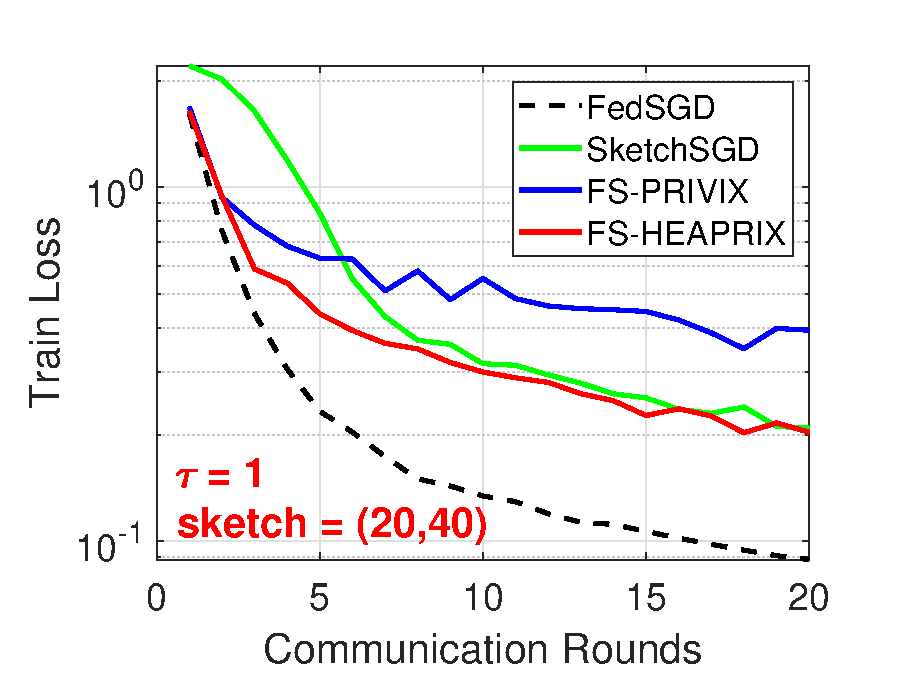
\includegraphics[width=2.2in]{MNIST_figures/local1_sketch20_iid1_train_loss.eps} 
		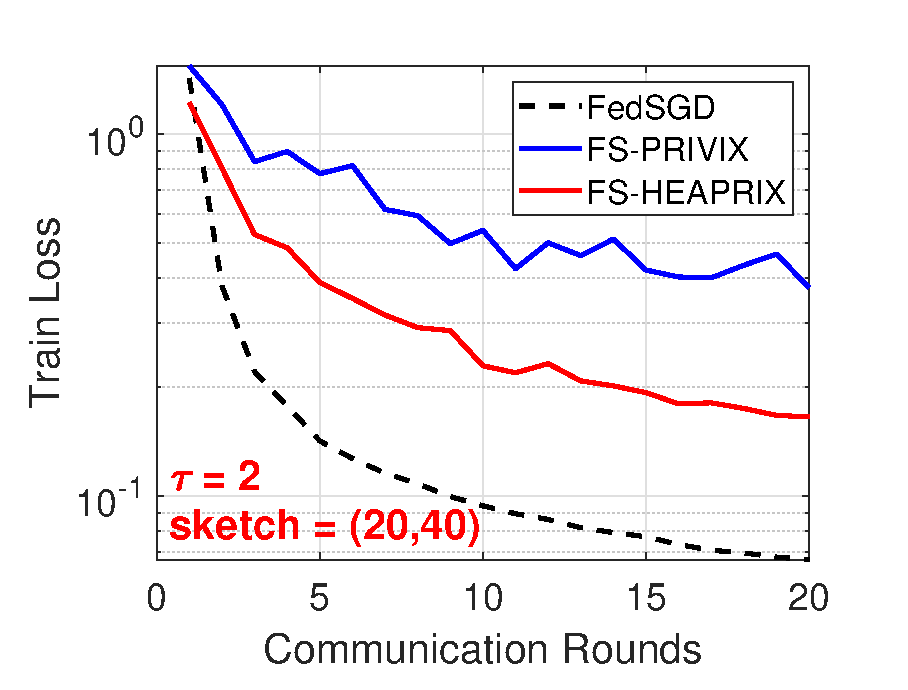
\includegraphics[width=2.2in]{MNIST_figures/local2_sketch20_iid1_train_loss.eps} 
		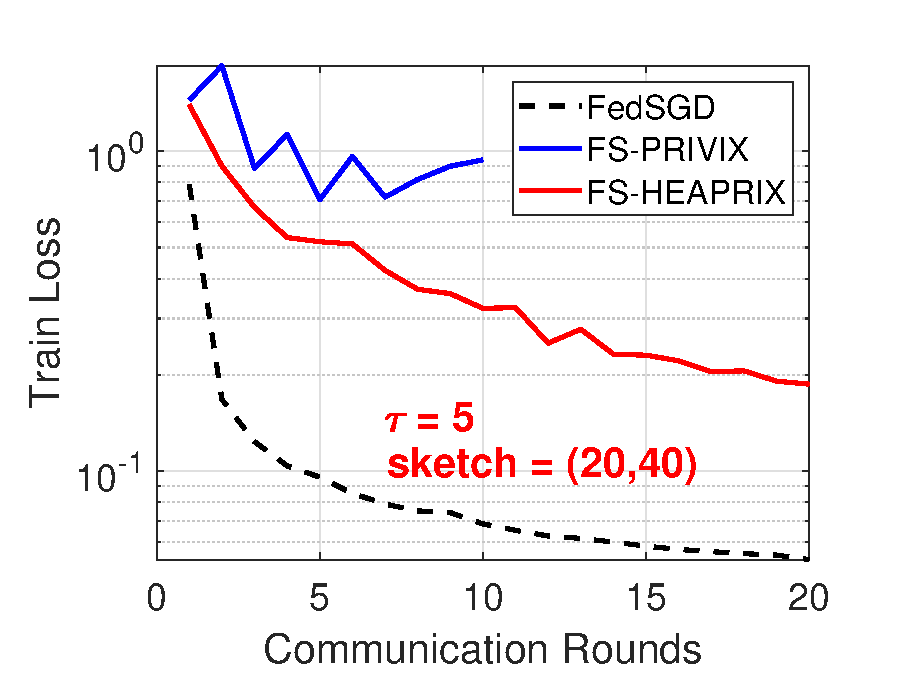
\includegraphics[width=2.2in]{MNIST_figures/local5_sketch20_iid1_train_loss.eps}}
		
		\mbox{%
		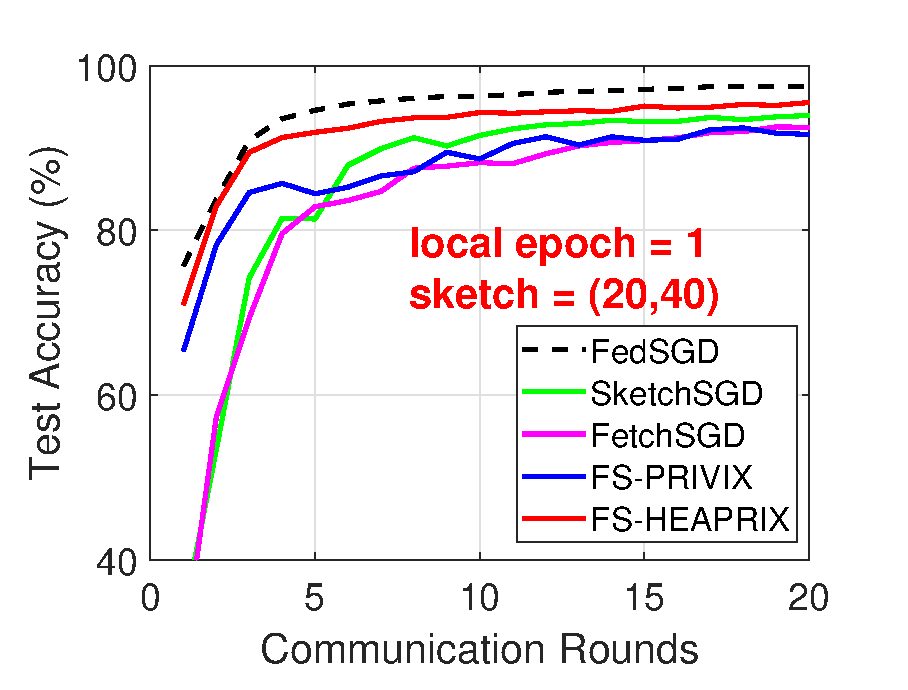
\includegraphics[width=2.2in]{MNIST_figures/local1_sketch20_iid1_test_acc.eps} %
		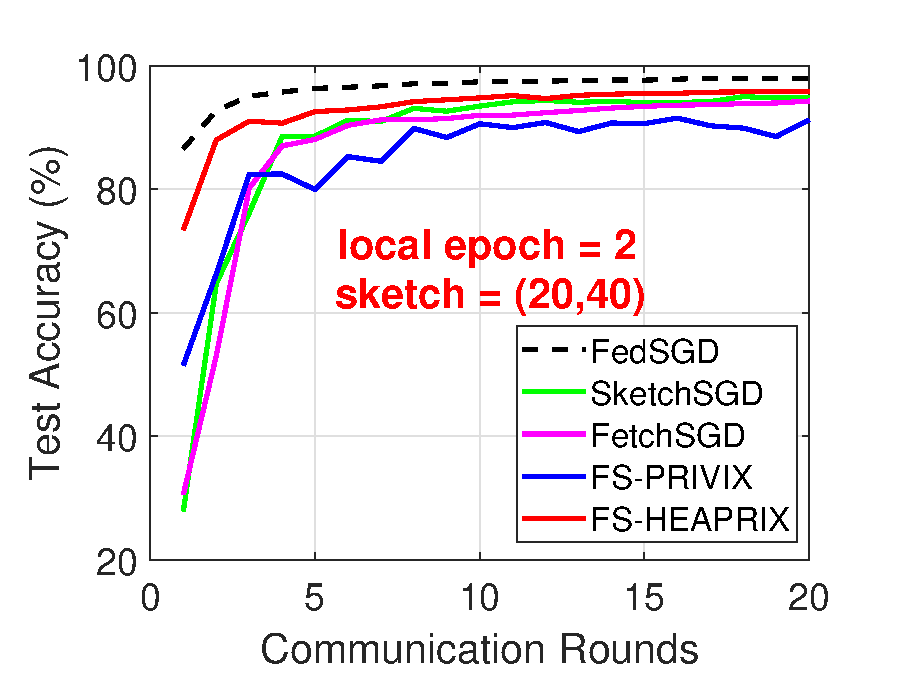
\includegraphics[width=2.2in]{MNIST_figures/local2_sketch20_iid1_test_acc.eps} %
		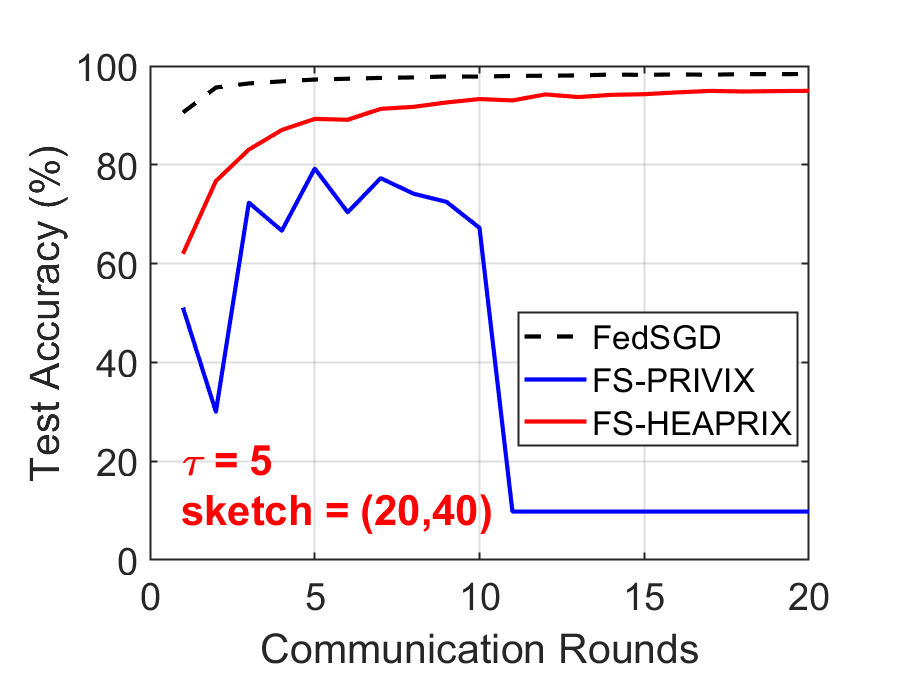
\includegraphics[width=2.2in]{MNIST_figures/local5_sketch20_iid1_test_acc.eps}%
		}
		\mbox{%	   
		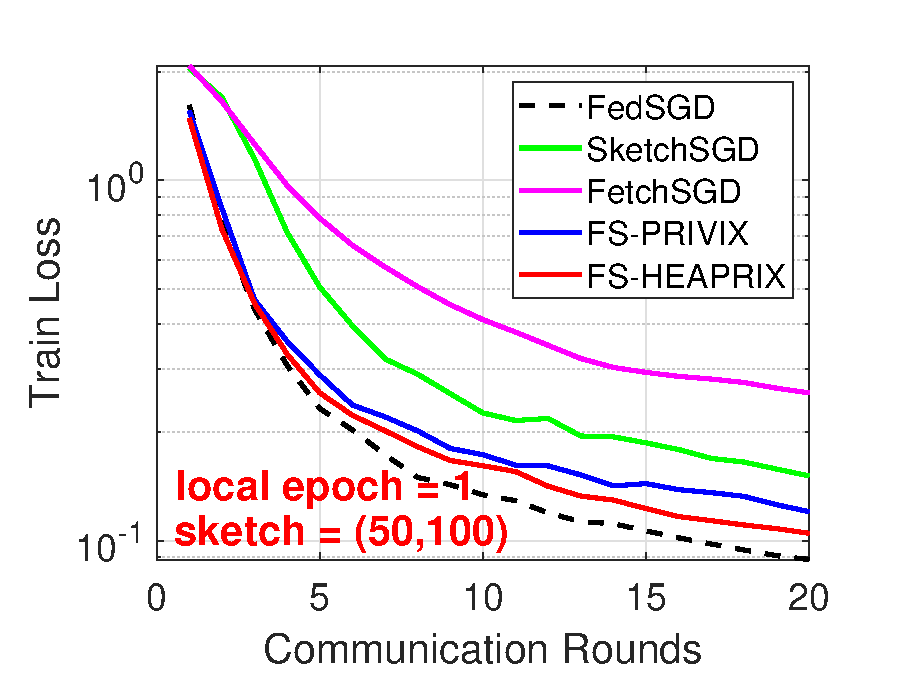
\includegraphics[width=2.2in]{MNIST_figures/local1_sketch50_iid1_train_loss.eps}% 
		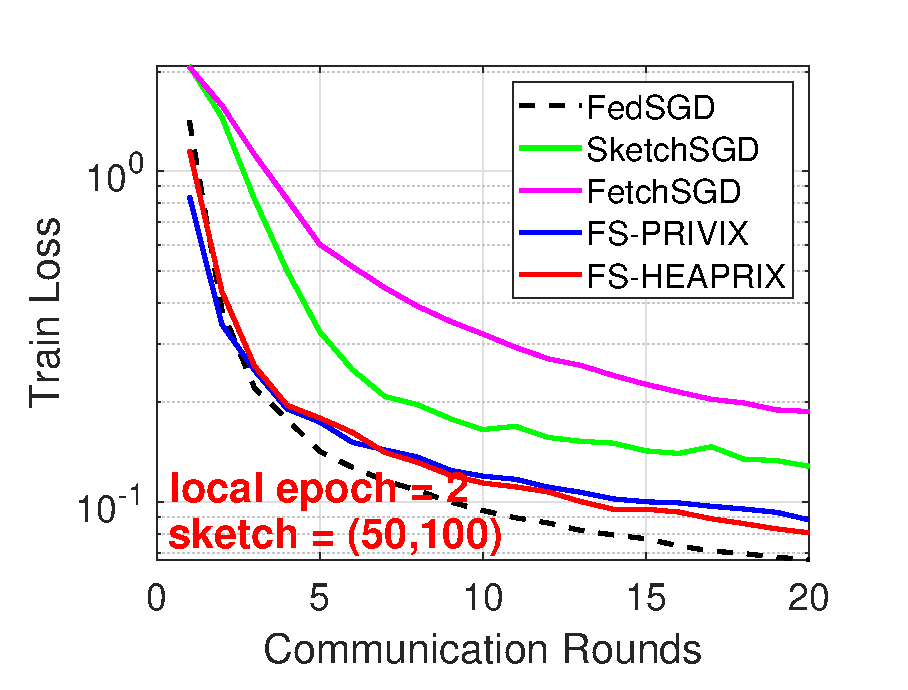
\includegraphics[width=2.2in]{MNIST_figures/local2_sketch50_iid1_train_loss.eps} %
		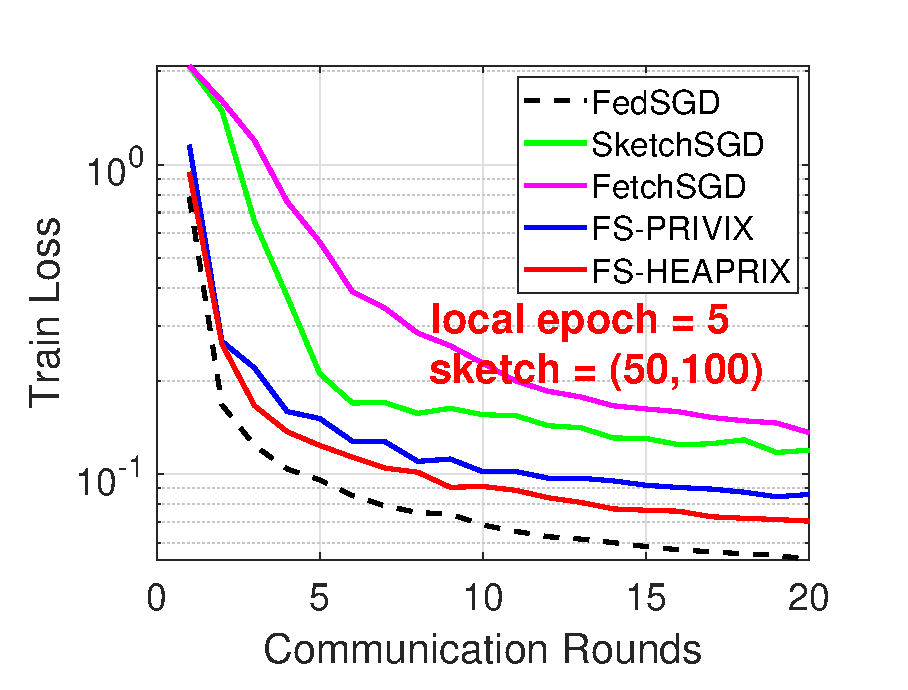
\includegraphics[width=2.2in]{MNIST_figures/local5_sketch50_iid1_train_loss.eps}}
		\mbox{%	
		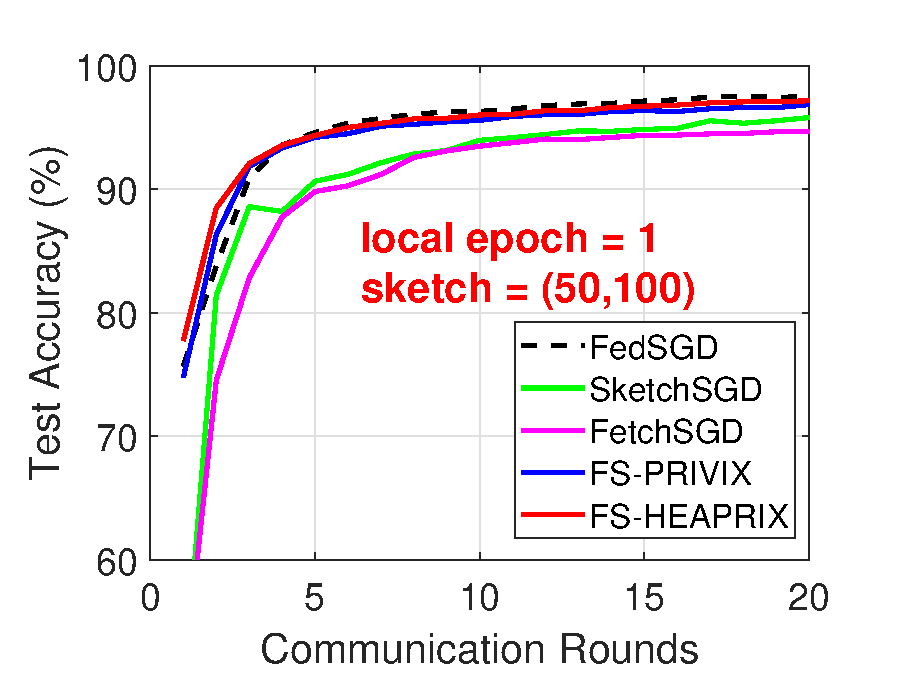
\includegraphics[width=2.2in]{MNIST_figures/local1_sketch50_iid1_test_acc.eps}% 
		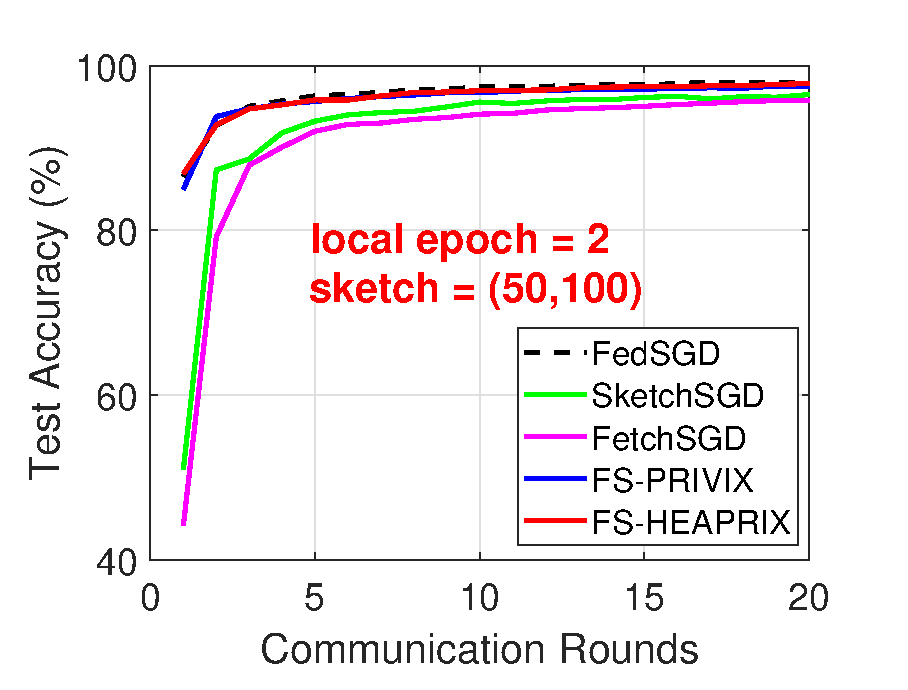
\includegraphics[width=2.2in]{MNIST_figures/local2_sketch50_iid1_test_acc.eps} %
		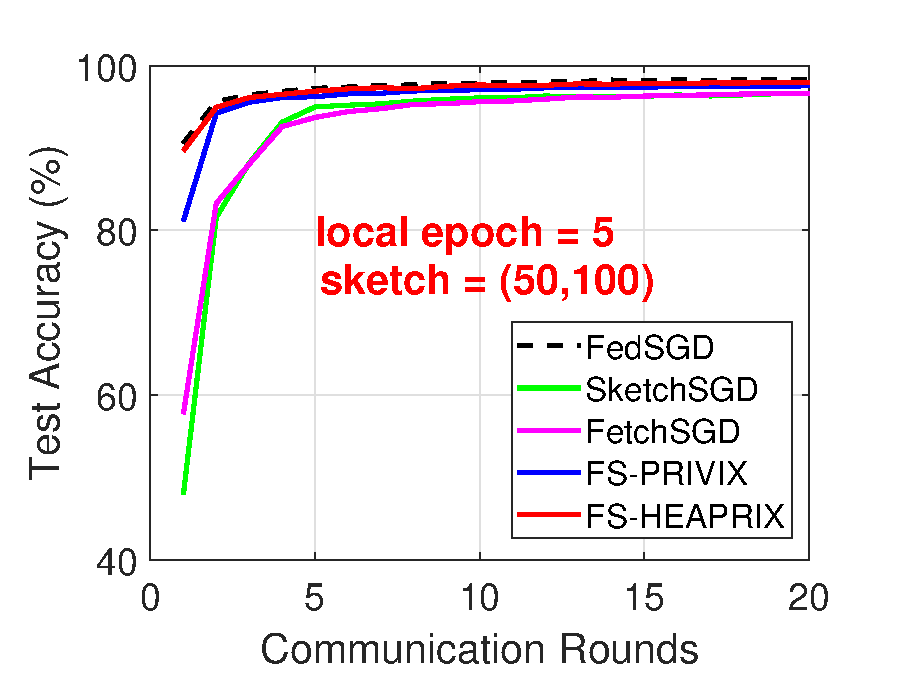
\includegraphics[width=2.2in]{MNIST_figures/local5_sketch50_iid1_test_acc.eps}
		}
	\end{center}
	\caption{MNIST Homogeneous case: Comparison of compressed optimization methods on LeNet CNN architecture.}
    \label{fig:MNIST-iid1-app}
\end{figure}

\subsubsection{Heterogeneous setting}

Analogously, we present experiments on MNIST dataset under heterogeneous data distribution, including $\tau=2$. We simulate the setting by only sending samples from one digit to each local worker (very few nodes get two classes). We see from Figure~\ref{fig:MNIST-iid0-app} that FS-HEAPRIX shows consistent advantage over competing methods. SketchedSGD performs poorly in this case.

\begin{figure}[h]
	\begin{center}
		\mbox{%			   
		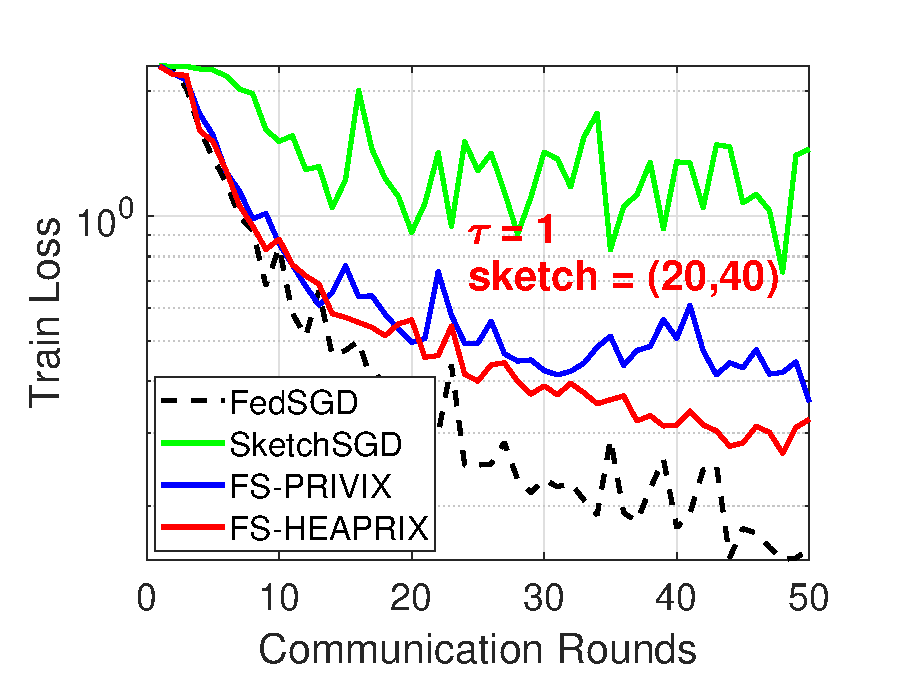
\includegraphics[width=2.2in]{MNIST_figures/local1_sketch20_iid0_train_loss.eps}% 
		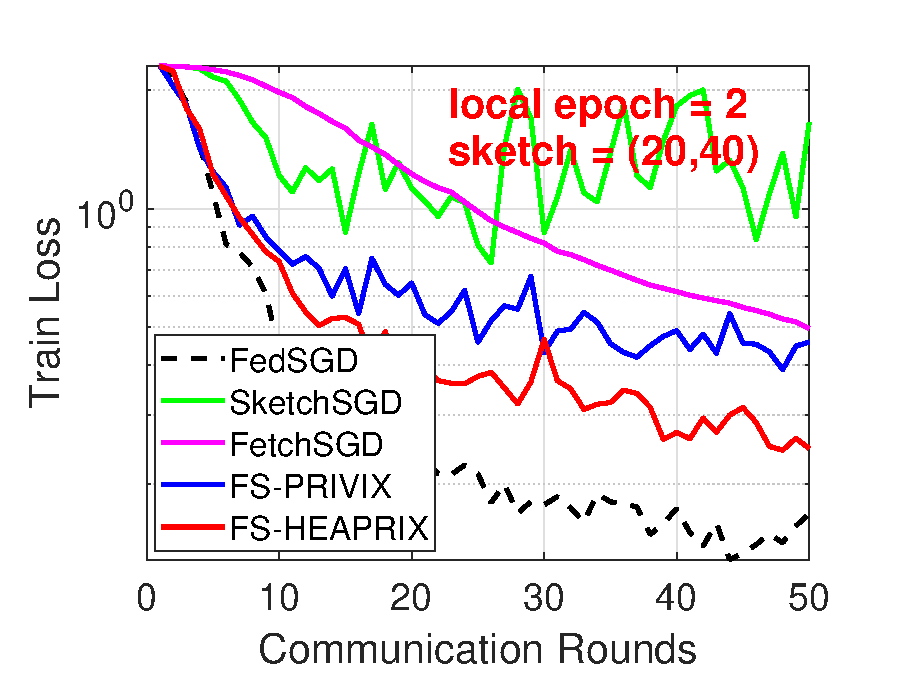
\includegraphics[width=2.2in]{MNIST_figures/local2_sketch20_iid0_train_loss.eps}% 
		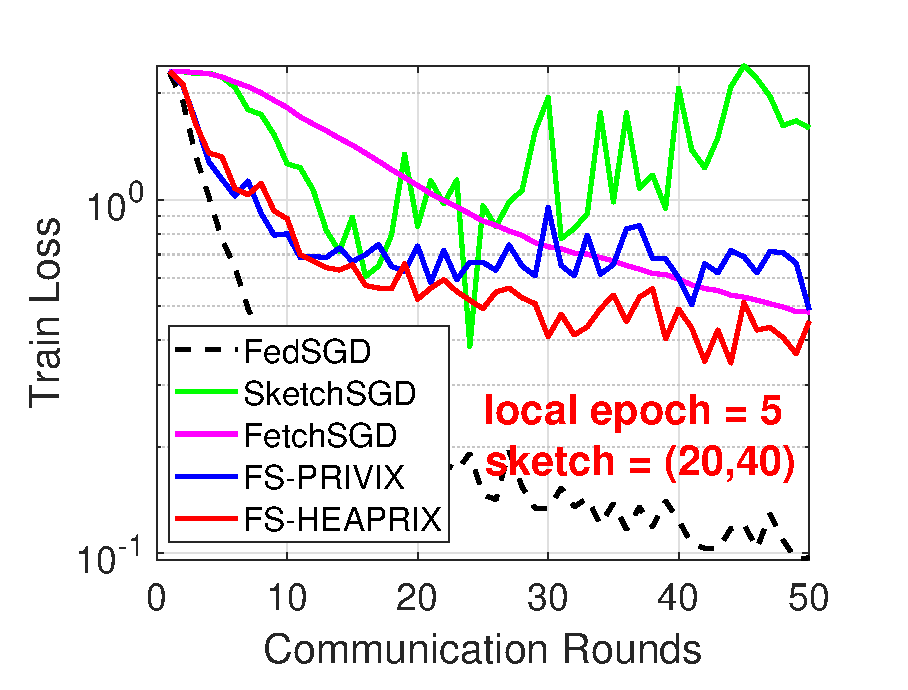
\includegraphics[width=2.2in]{MNIST_figures/local5_sketch20_iid0_train_loss.eps} }
		
		\mbox{%	
		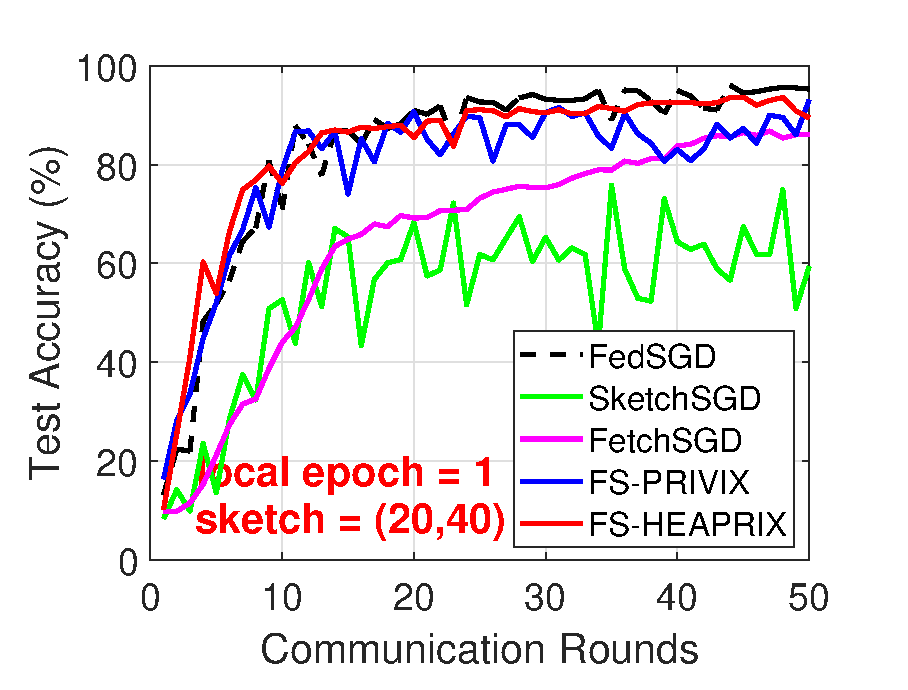
\includegraphics[width=2.2in]{MNIST_figures/local1_sketch20_iid0_test_acc.eps} %
		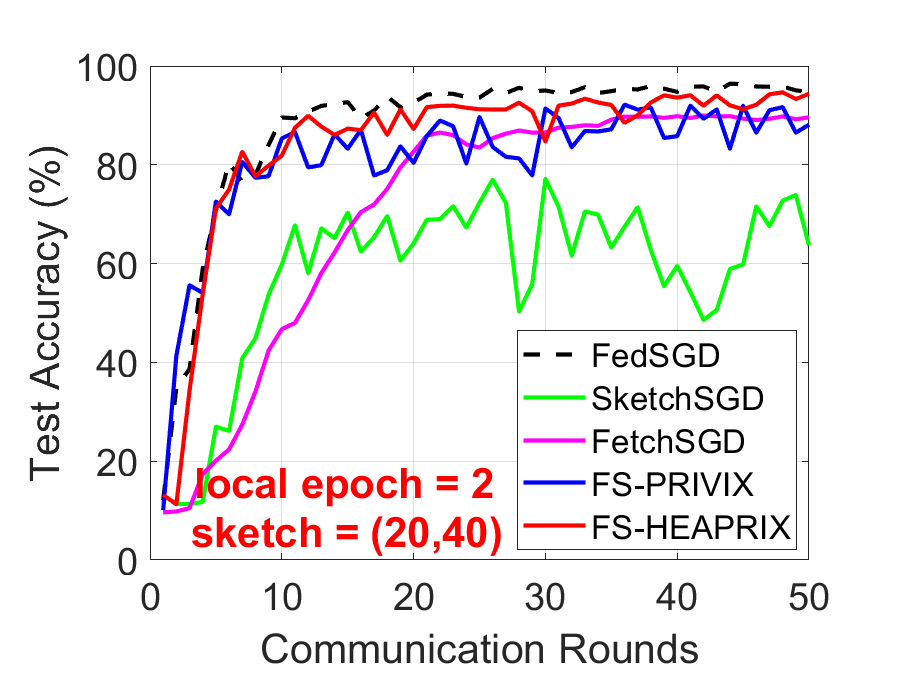
\includegraphics[width=2.2in]{MNIST_figures/local2_sketch20_iid0_test_acc.eps} %
		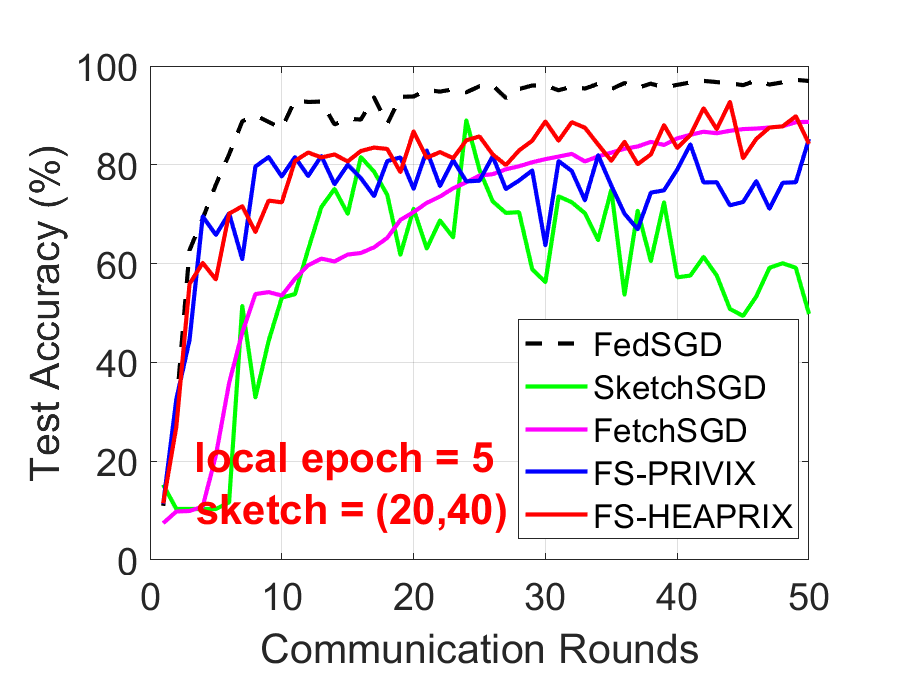
\includegraphics[width=2.2in]{MNIST_figures/local5_sketch20_iid0_test_acc.eps}
		}
		
		\mbox{%	  
		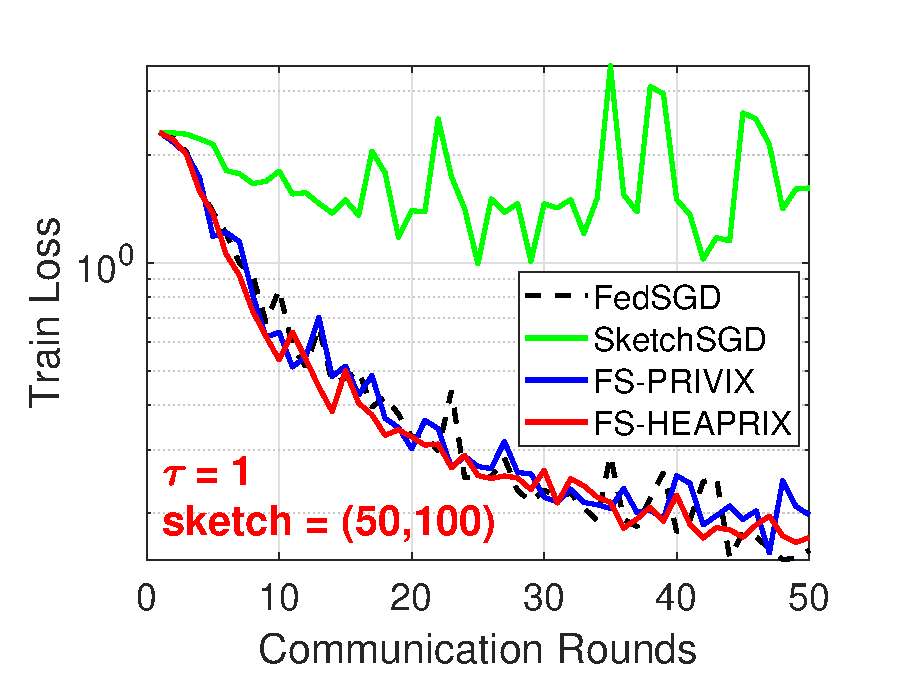
\includegraphics[width=2.2in]{MNIST_figures/local1_sketch50_iid0_train_loss.eps}% 
		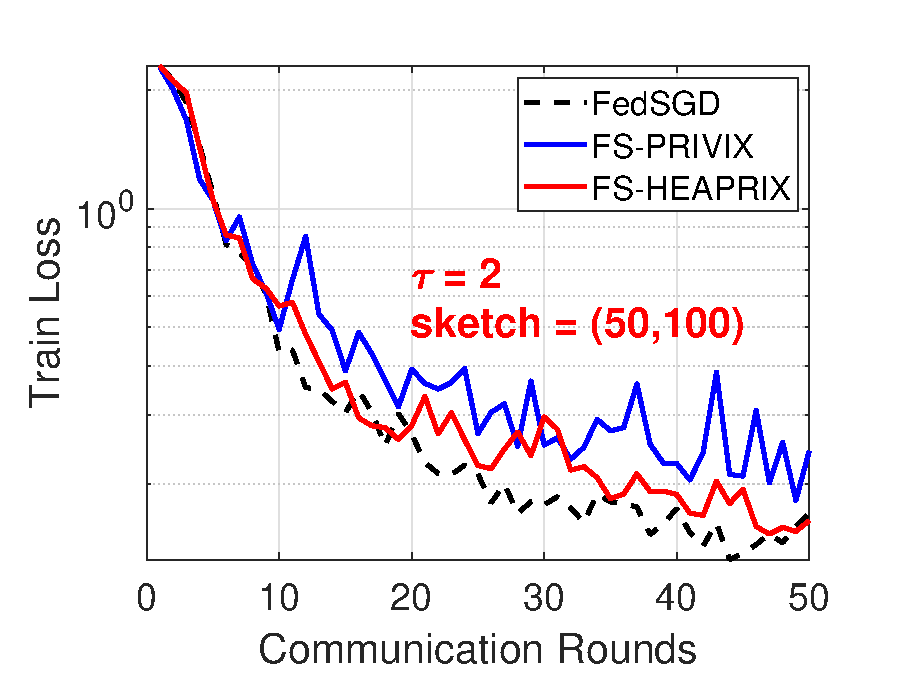
\includegraphics[width=2.2in]{MNIST_figures/local2_sketch50_iid0_train_loss.eps}% 
		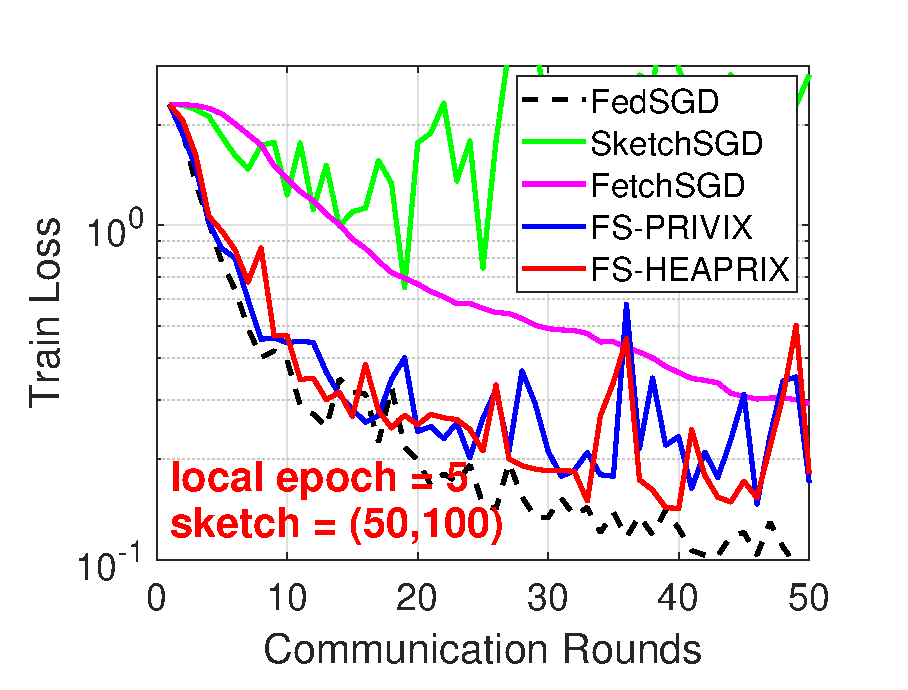
\includegraphics[width=2.2in]{MNIST_figures/local5_sketch50_iid0_train_loss.eps}}
		
		\mbox{%	
		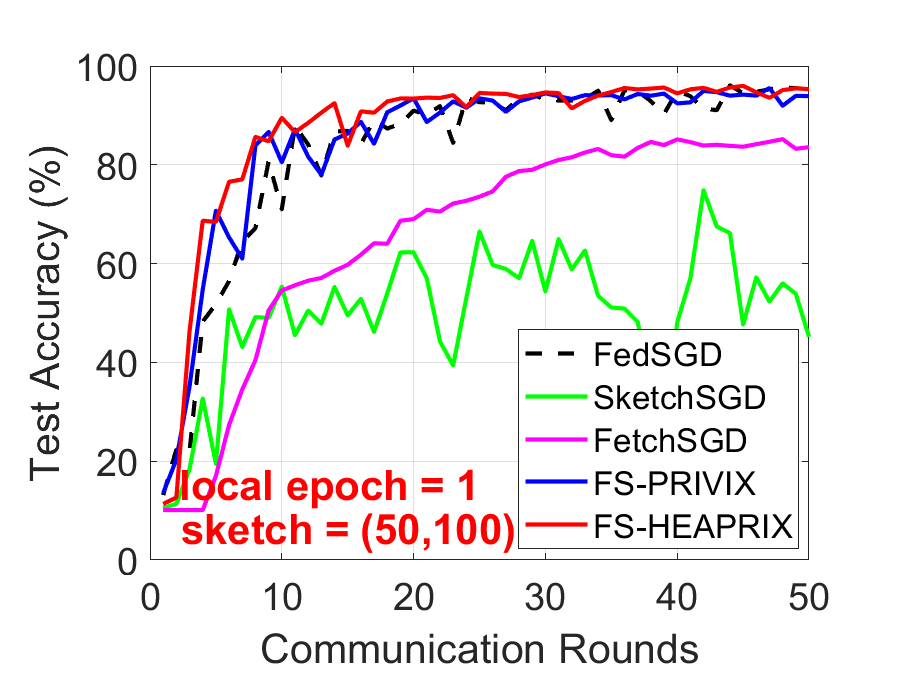
\includegraphics[width=2.2in]{MNIST_figures/local1_sketch50_iid0_test_acc.eps}% 
		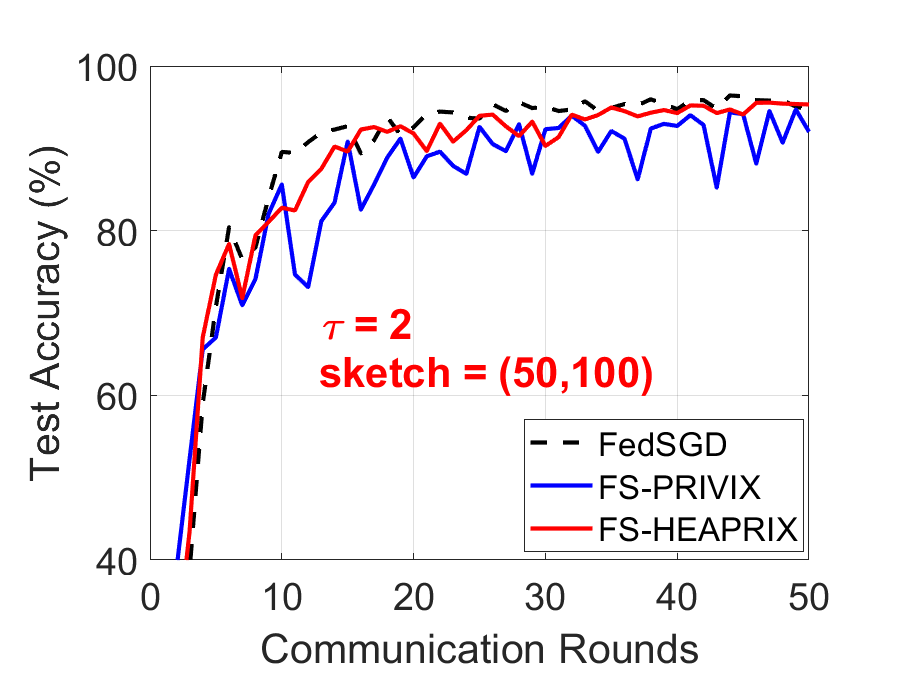
\includegraphics[width=2.2in]{MNIST_figures/local2_sketch50_iid0_test_acc.eps} %
		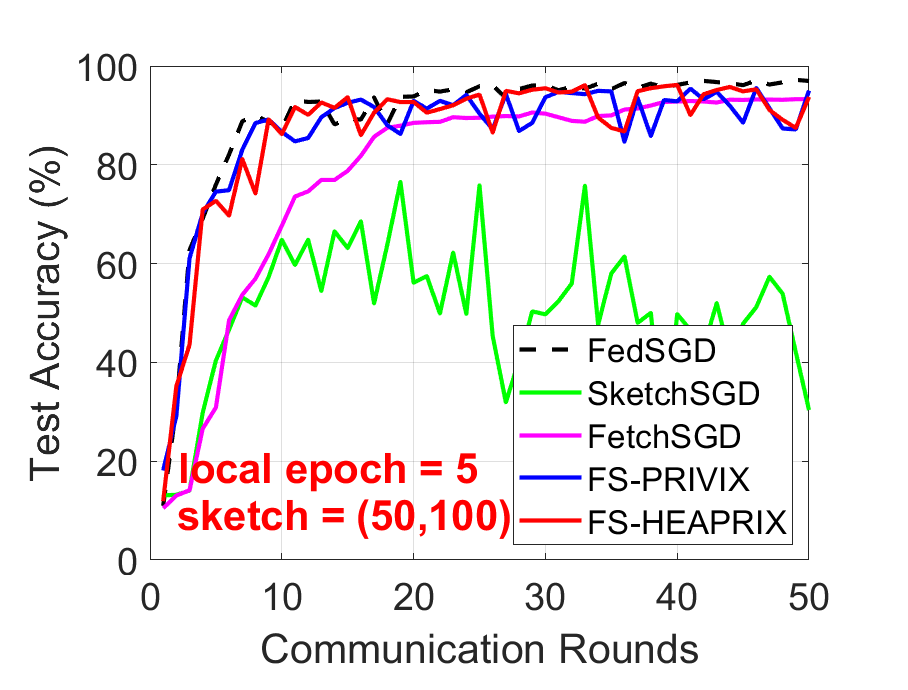
\includegraphics[width=2.2in]{MNIST_figures/local5_sketch50_iid0_test_acc.eps}
		}
	\end{center}
	\caption{MNIST Heterogeneous case: Comparison of compressed optimization algorithms on LeNet CNN architecture.}
    \label{fig:MNIST-iid0-app}
\end{figure}


\newpage
\subsection{Additional Experiments: CIFAR-10}


We conduct similar sets of experiments on CIFAR10 dataset. We also use the simple LeNet CNN structure, as in practice small models are more favorable in federated learning, due to the limitation of mobile devices. The test accuracy is presented in Figure~\ref{fig:CIFAR-homog} and Figure~\ref{fig:CIFAR-heter}, for respectively homogeneous and heterogeneous data distribution. In general, we retrieve similar information as from MNIST experiments: our proposed FS-HEAPRIX improves FS-PRIVIX and SketchedSGD in all cases. We note that although the test accuracy provided by LeNet cannot reach the state-of-the-art accuracy given by some huge models, it is also informative in terms of comparing the relative performance of different sketching methods.



\begin{figure}[h]
	\begin{center}
		\mbox{%			   
		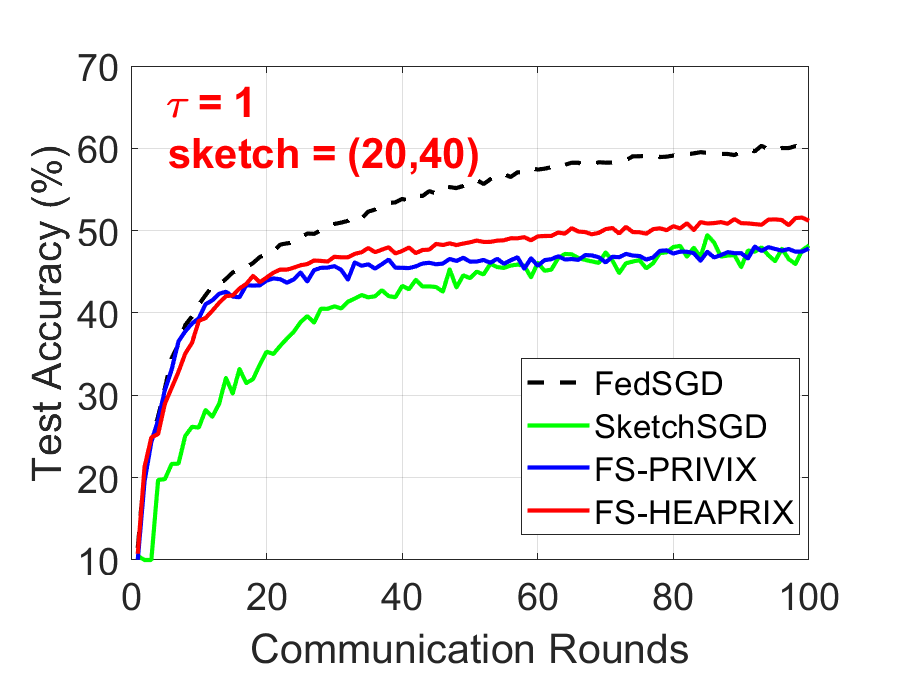
\includegraphics[width=3.0in]{CIFAR_figures/cifar_local1_sketch20_iid1_test_acc.eps}  
		 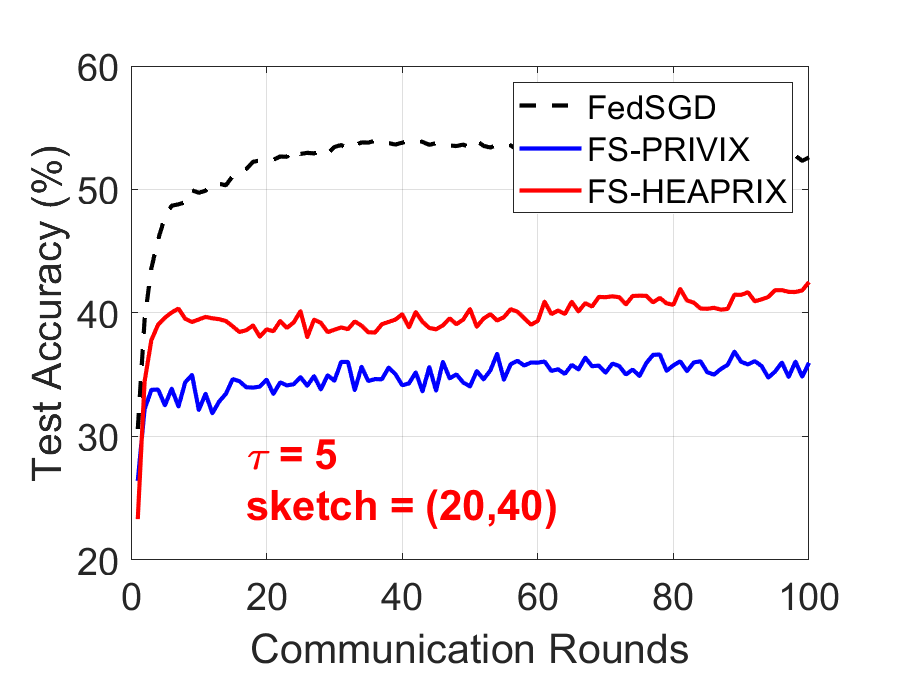
\includegraphics[width=3.0in]{CIFAR_figures/cifar_local5_sketch20_iid1_test_acc.eps}
		}
		\mbox{%	
	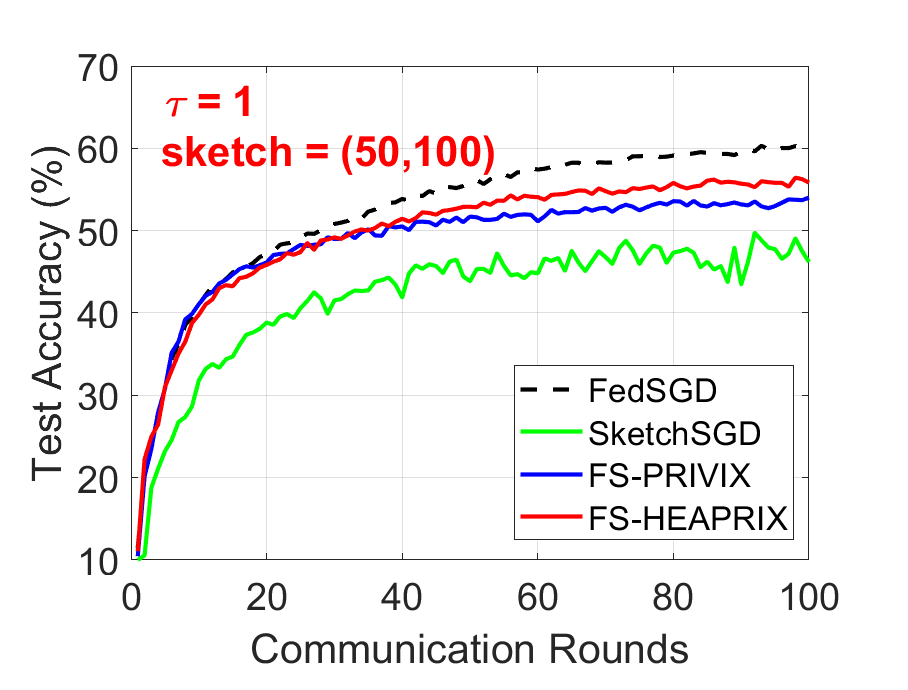
\includegraphics[width=3.0in]{CIFAR_figures/cifar_local1_sketch50_iid1_test_acc.eps} 
		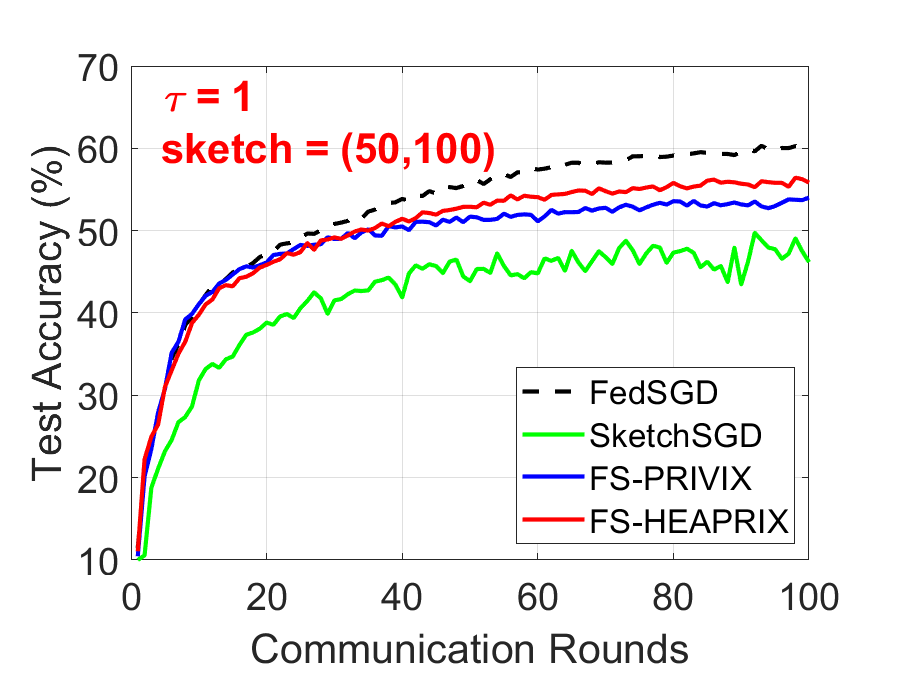
\includegraphics[width=3.0in]{CIFAR_figures/cifar_local5_sketch50_iid1_test_acc.eps}
		}
	\end{center}
	\caption{Homogeneous case: CIFAR10: Comparison of compressed optimization methods on LeNet CNN.}
    \label{fig:CIFAR-homog}
\end{figure}



\begin{figure}[h]
	\begin{center}
		\mbox{%			   
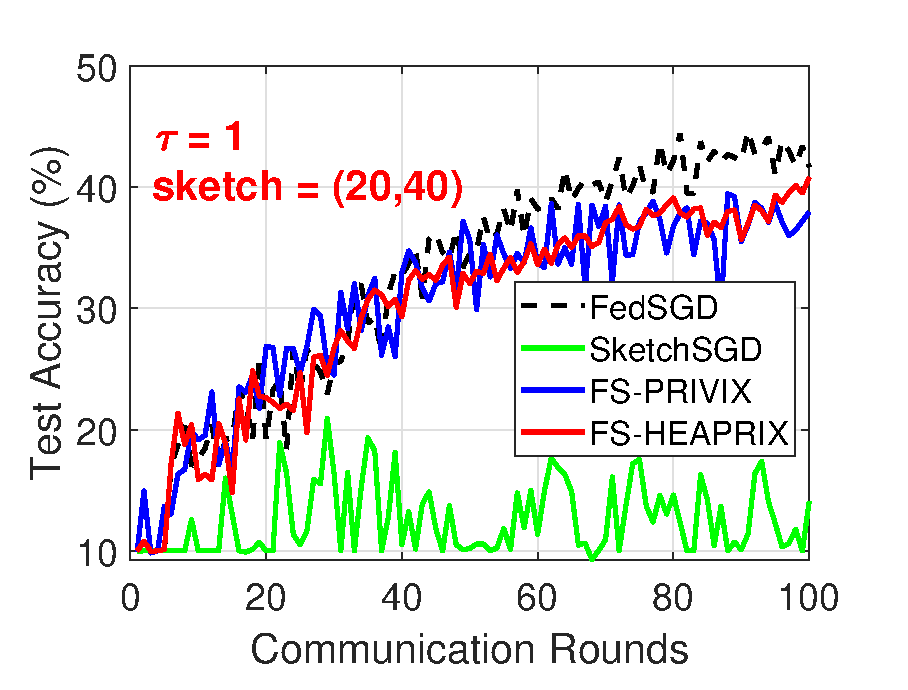
\includegraphics[width=3.0in]{CIFAR_figures/cifar_local1_sketch20_iid0_test_acc.eps} 
		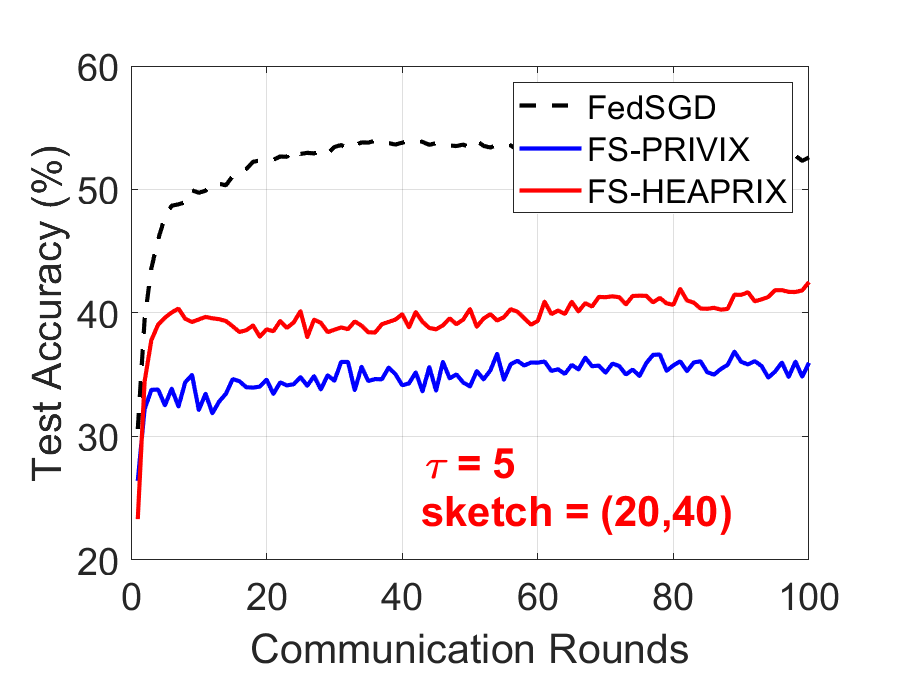
\includegraphics[width=3.0in]{CIFAR_figures/cifar_local5_sketch20_iid0_test_acc.eps}
		}
		\mbox{%	
		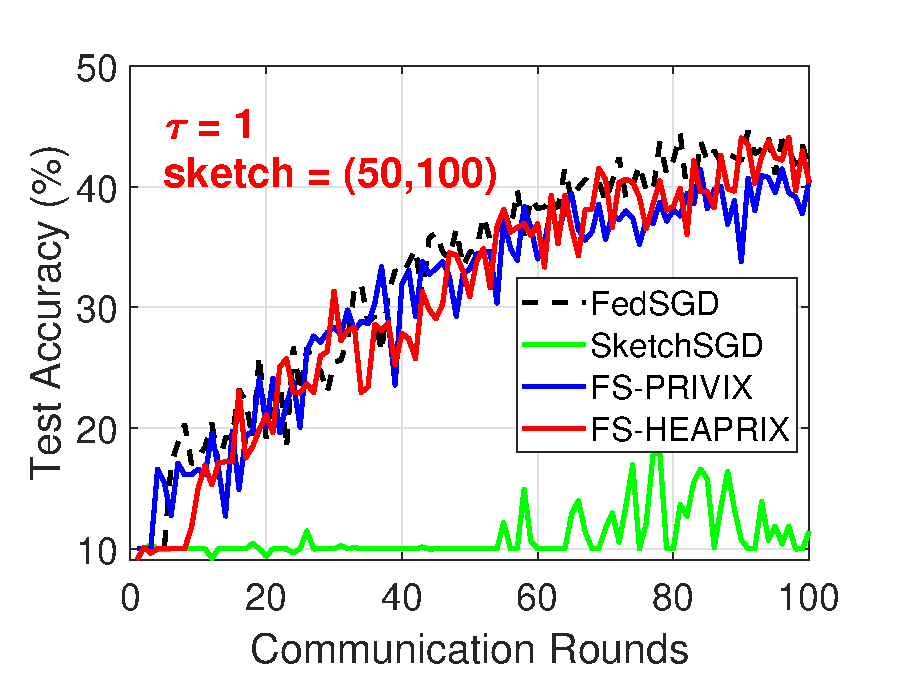
\includegraphics[width=3.0in]{CIFAR_figures/cifar_local1_sketch50_iid0_test_acc.eps}
		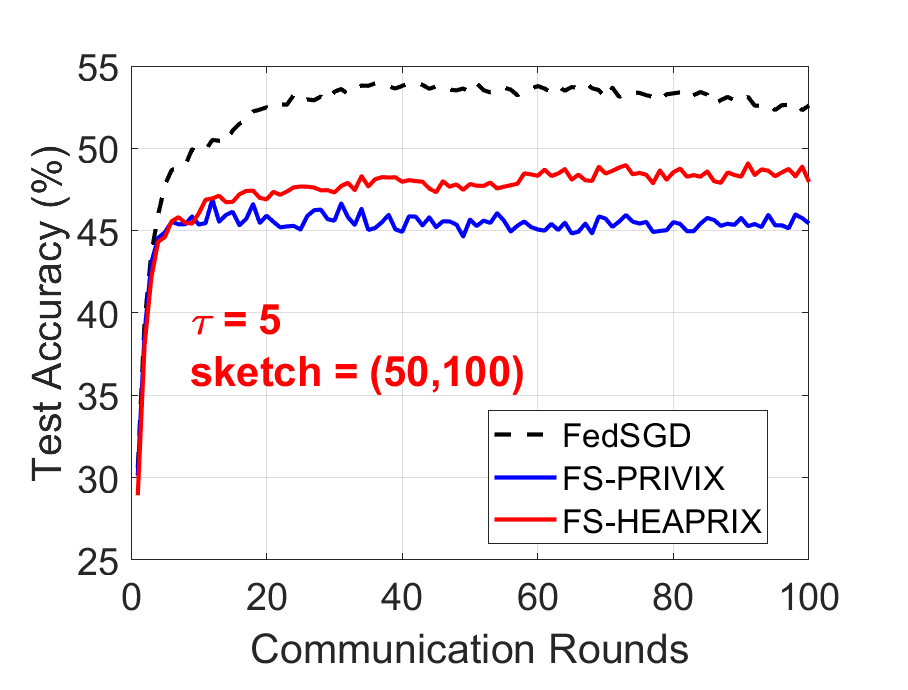
\includegraphics[width=3.0in]{CIFAR_figures/cifar_local5_sketch50_iid0_test_acc.eps}
		}
	\end{center}
	\caption{Heterogeneous case: CIFAR10: Comparison of compressed optimization methods on LeNet CNN.}
    \label{fig:CIFAR-heter}
\end{figure}



%We conduct similar sets of experiments on CIFAR10 dataset. We also use the simple LeNet CNN structure, as in practice small models are more favorable in federated learning, due to the limitation of mobile devices. The test accuracy is presented in Figure~\ref{fig:CIFAR}, for both homogeneous and heterogeneous data distribution. In general, we retrieve similar information as from MNIST experiments: our proposed FS-HEAPRIX improves FS-PRIVIX and SketchedSGD in all cases. We note that although the test accuracy provided by LeNet cannot reach the state-of-the-art accuracy given by some huge models, it is also informative in terms of comparing the relative performance of different sketching methods.

%\begin{figure}[h]
%	\begin{center}
%		\subfigure[CIFAR10 Homogeneous case.]{
%		\mbox{			  
%		 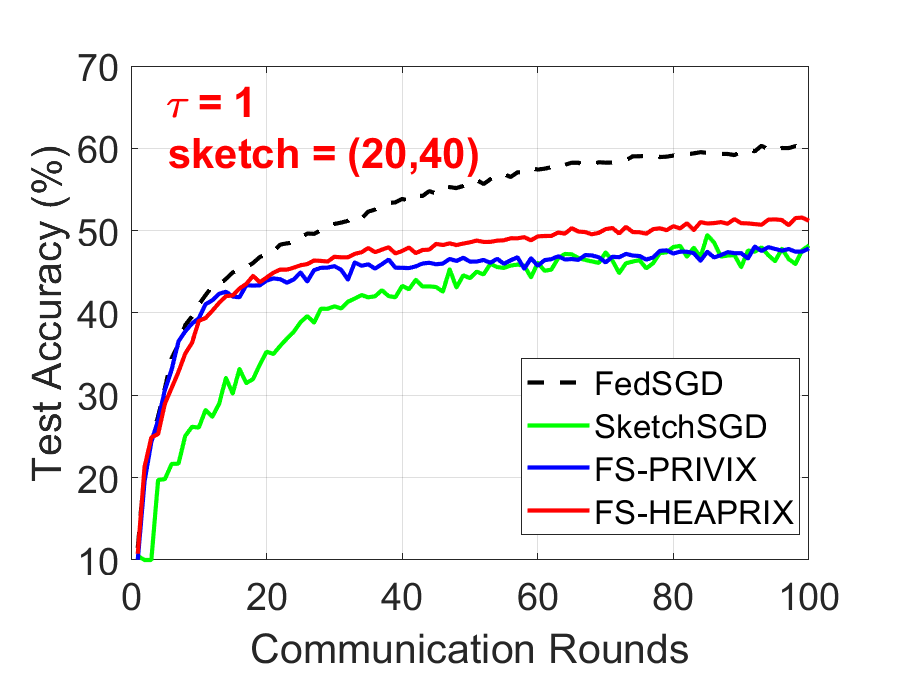
\includegraphics[width=1.7in]{CIFAR_figures/cifar_local1_sketch20_iid1_test_acc.eps}  
%		 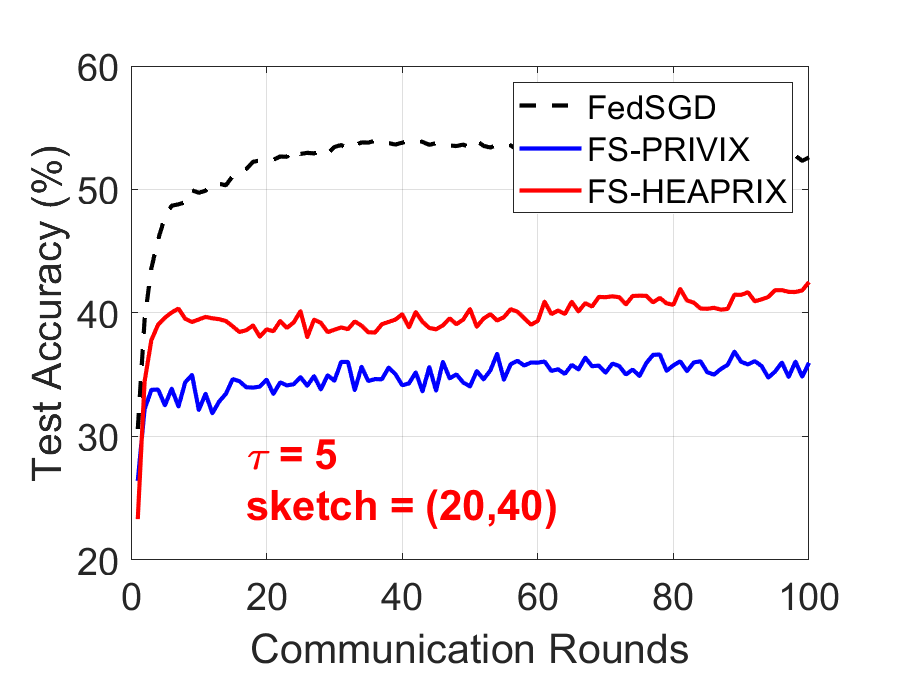
\includegraphics[width=1.7in]{CIFAR_figures/cifar_local5_sketch20_iid1_test_acc.eps}
%		\includegraphics[width=1.7in]{CIFAR_figures/cifar_local1_sketch50_iid1_test_acc.eps} 
%		\includegraphics[width=1.7in]{CIFAR_figures/cifar_local5_sketch50_iid1_test_acc.eps}
%
%		}
%		}
%		\subfigure[CIFAR10 Heterogeneous case.]{
%
%	
%		\mbox{	
%		\includegraphics[width=1.7in]{CIFAR_figures/cifar_local1_sketch20_iid0_test_acc.eps} 
%		\includegraphics[width=1.7in]{CIFAR_figures/cifar_local5_sketch20_iid0_test_acc.eps}
%		\includegraphics[width=1.7in]{CIFAR_figures/cifar_local1_sketch50_iid0_test_acc.eps}
%		\includegraphics[width=1.7in]{CIFAR_figures/cifar_local5_sketch50_iid0_test_acc.eps}
%		}
%		}
%	\end{center}
%	\caption{CIFAR10: Comparison of compressed optimization methods on LeNet CNN.}
%    \label{fig:CIFAR}
%\end{figure}




\end{document}

